\chapter{Ancillary Model Performance Analyses}

\section{Bayesian Multi-Level Model Definition}
\label{bayesian_multilevel_model}
In order to assess in a more robust and reliable way the results of our models comparison experiments, along with the conventional frequentist analyses presented in chapter \ref{chapter_implementation_testing} we carried out an additional set of statistical analyses using a bespoke Bayesian multi-level model. We opted for a time-varying random intercept accounting for the impact of game context and time and a fixed slope for estimating the effect of model architecture. We adopted a partial pooling strategy for the time-varying random intercept as we could safely assume exchangeability of parameters for the various game contexts \cite{gelman2020bayesian}. The model had the following formulation:
\begin{gather}
    \label{bayesian_mlm}
    SMAPE_{i, j, t} \sim StudentT(\nu, \mu, \sigma) \\ \nonumber
    \nu \sim Gamma(\alpha=2, \beta=0.1) \\ \nonumber
    \sigma \sim HalfCaucy(\beta=1)  \\ \nonumber
    \mu = \beta_{jt} + \alpha_{i}  \\ \nonumber
    \alpha_{i} \sim Normal(\mu=0, \sigma=1)  \\ \nonumber
    \beta_{jt} = \alpha_{j}^\top B_{t,*} \\ \nonumber
    \alpha_{j} \sim Normal(\mu_j, \sigma_j) \\ \nonumber
    \mu_j \sim Normal(\mu=1, \sigma=1) \\ \nonumber
    \sigma_j \sim HalfCauchy(\beta=1) \\ \nonumber
\end{gather}
with $B \in \mathbb{R}^{T \times dof}$ being a cubic B-spline matrix with $dof=6$ as provided by the python library Patsy \cite{patsy}. In this case $j$ indicates the $j^{\text{th}}$ game context, $i$ the $i^{\text{th}}$ model and $t$ the $t^{\text{th}}$ element in the considered sequence of SMAPE values. The $StudentT$ likelyhood allowed for an estimation of $\mu$ robust to outliers. The values for the the $Gamma$ distribution parameters were chosen according to a sensible default as mentioned in \cite{vehtarinu}. The choice of priors for $\alpha_{i}$ were made so to have a small regularizing effect: the priors assume each model to have an impact on the base SMAPE of $\sim \pm 2\% $ but with the expectancy of having no effect. The same model was fit first collapsing all the target in a single overall performance metric and then separately on each of the 5 targets. In order to estimate parameters for the model we used mean field approximation \cite{kucukelbir2017automatic}. The model was implemented using the python library PyMC3 \cite{salvatier2016probabilistic}. As mean field approximation doesn't allow conventional convergence checks for Bayesian model fitting, we relied exclusively on visual inspection of the marginal probability distributions. Comparison between different models was carried out by inspecting the marginal distribution of differences in the $\mu$ parameter, highlighting a region of practical significance (ROPE) equals to $\{-0.1, 0.1\}$. This means that we deemed worth of attention only differences in $\mu$ greater than $0.1\%$ SMAPE.

\section{Dynamic Prediction of Future Behavioural Intensity}
\label{dynamic_prediction_ancillary_perf}

We report here the results of fitting the Bayesian model to the perfromance data obtained from the experimental task described in section \ref{model_architecture_2}.

\subsection{Targets Collapsed}
\label{collapsed_bayes_2}

\begin{figure}[ht]
\centering
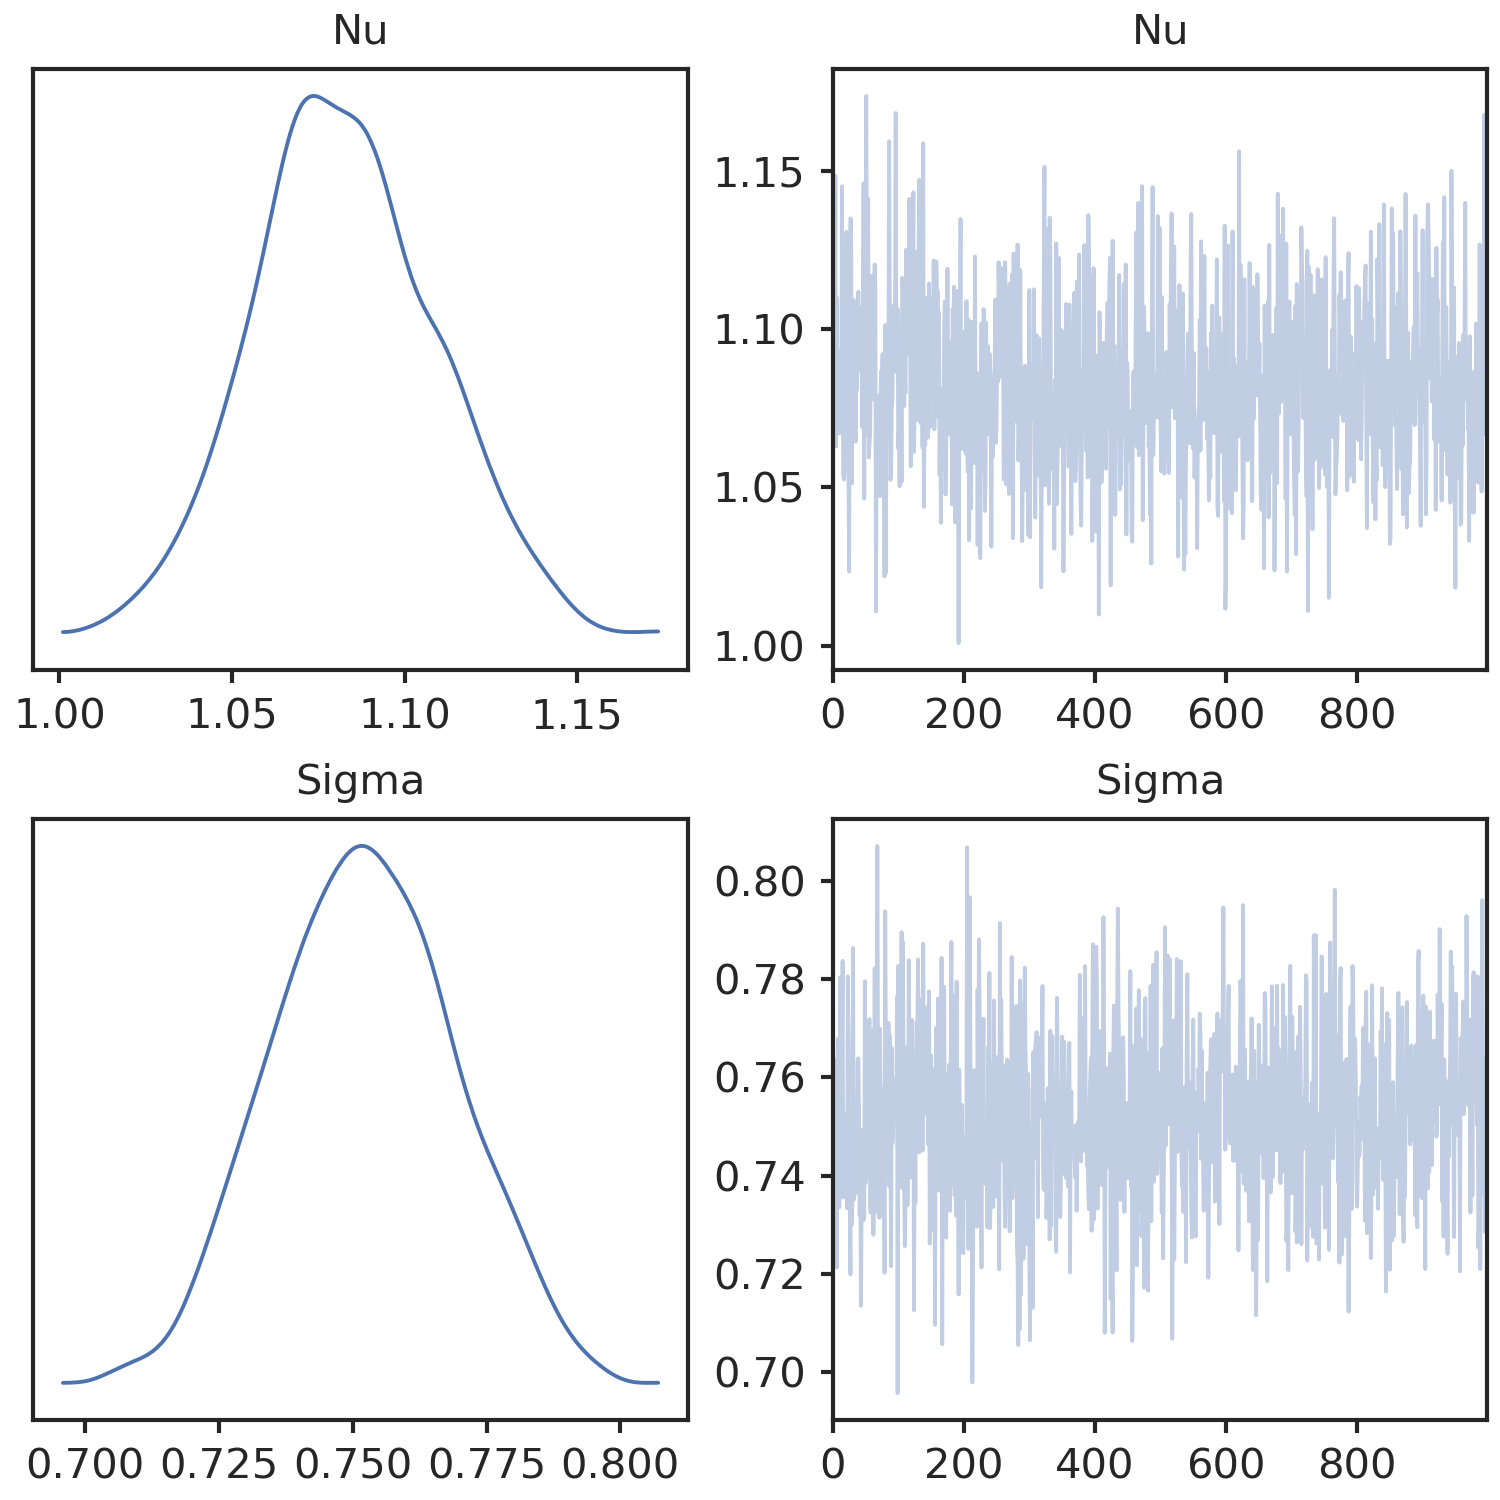
\includegraphics[width=0.5\textwidth]{images/appendix_C/collapsed_marginals_2.png}
\caption[\textbf{Targets collapsed marginal distributions}]{Marginal distributions for the parameters $\nu$, $\sigma$ estimated by the model fitted for the Future Absence target.}
\label{marginals_coll_2}
\end{figure}
\FloatBarrier

\begin{figure}[ht]
\centering
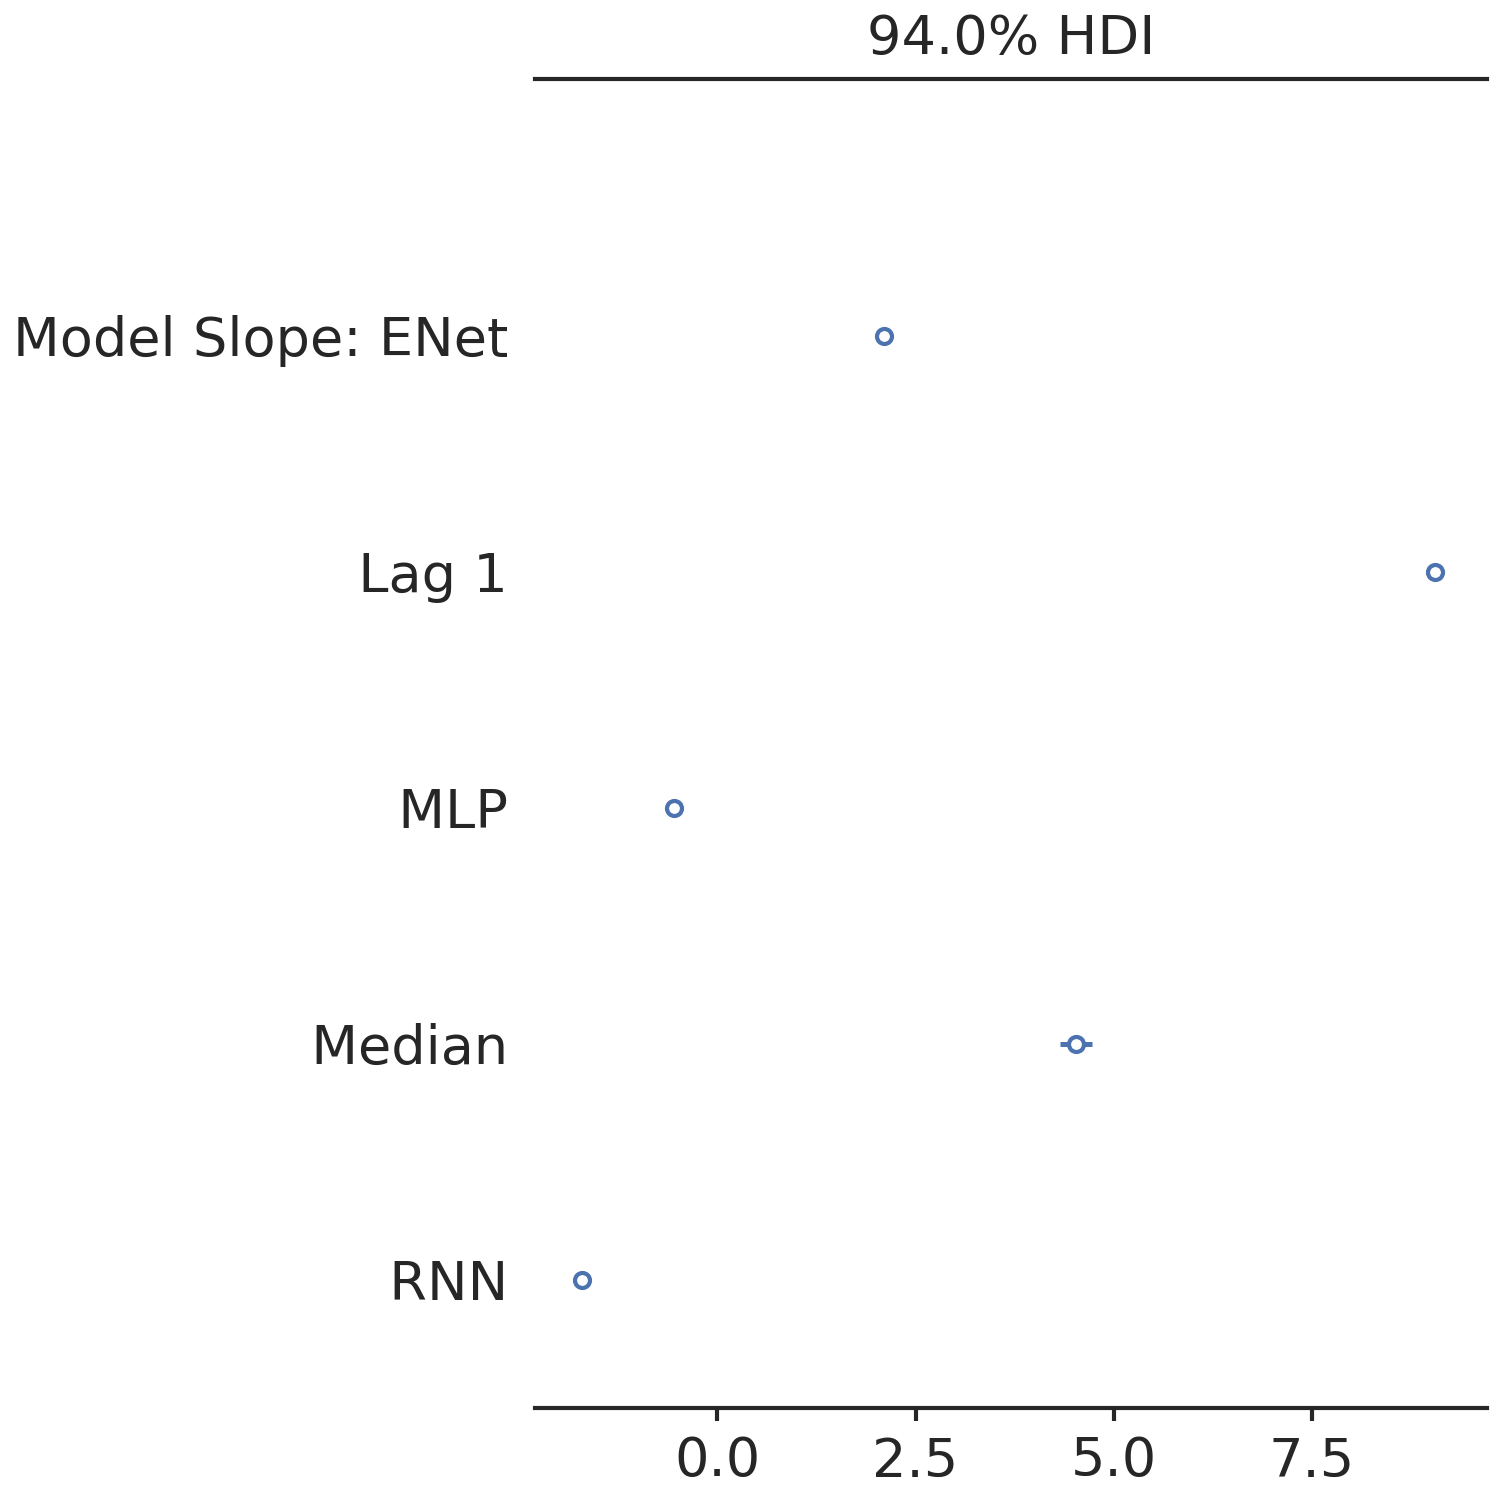
\includegraphics[width=0.5\textwidth]{images/appendix_C/collapsed_models_2.png}
\caption[\textbf{Targets collapsed model fixed effect}]{Forest plot of the marginal distributions for the parameter $\alpha$ (i.e. model slope) estimated by the model fitted for the Future Absence target.}
\label{model_coll_2}
\end{figure}
\FloatBarrier

\begin{figure}[ht]
\centering
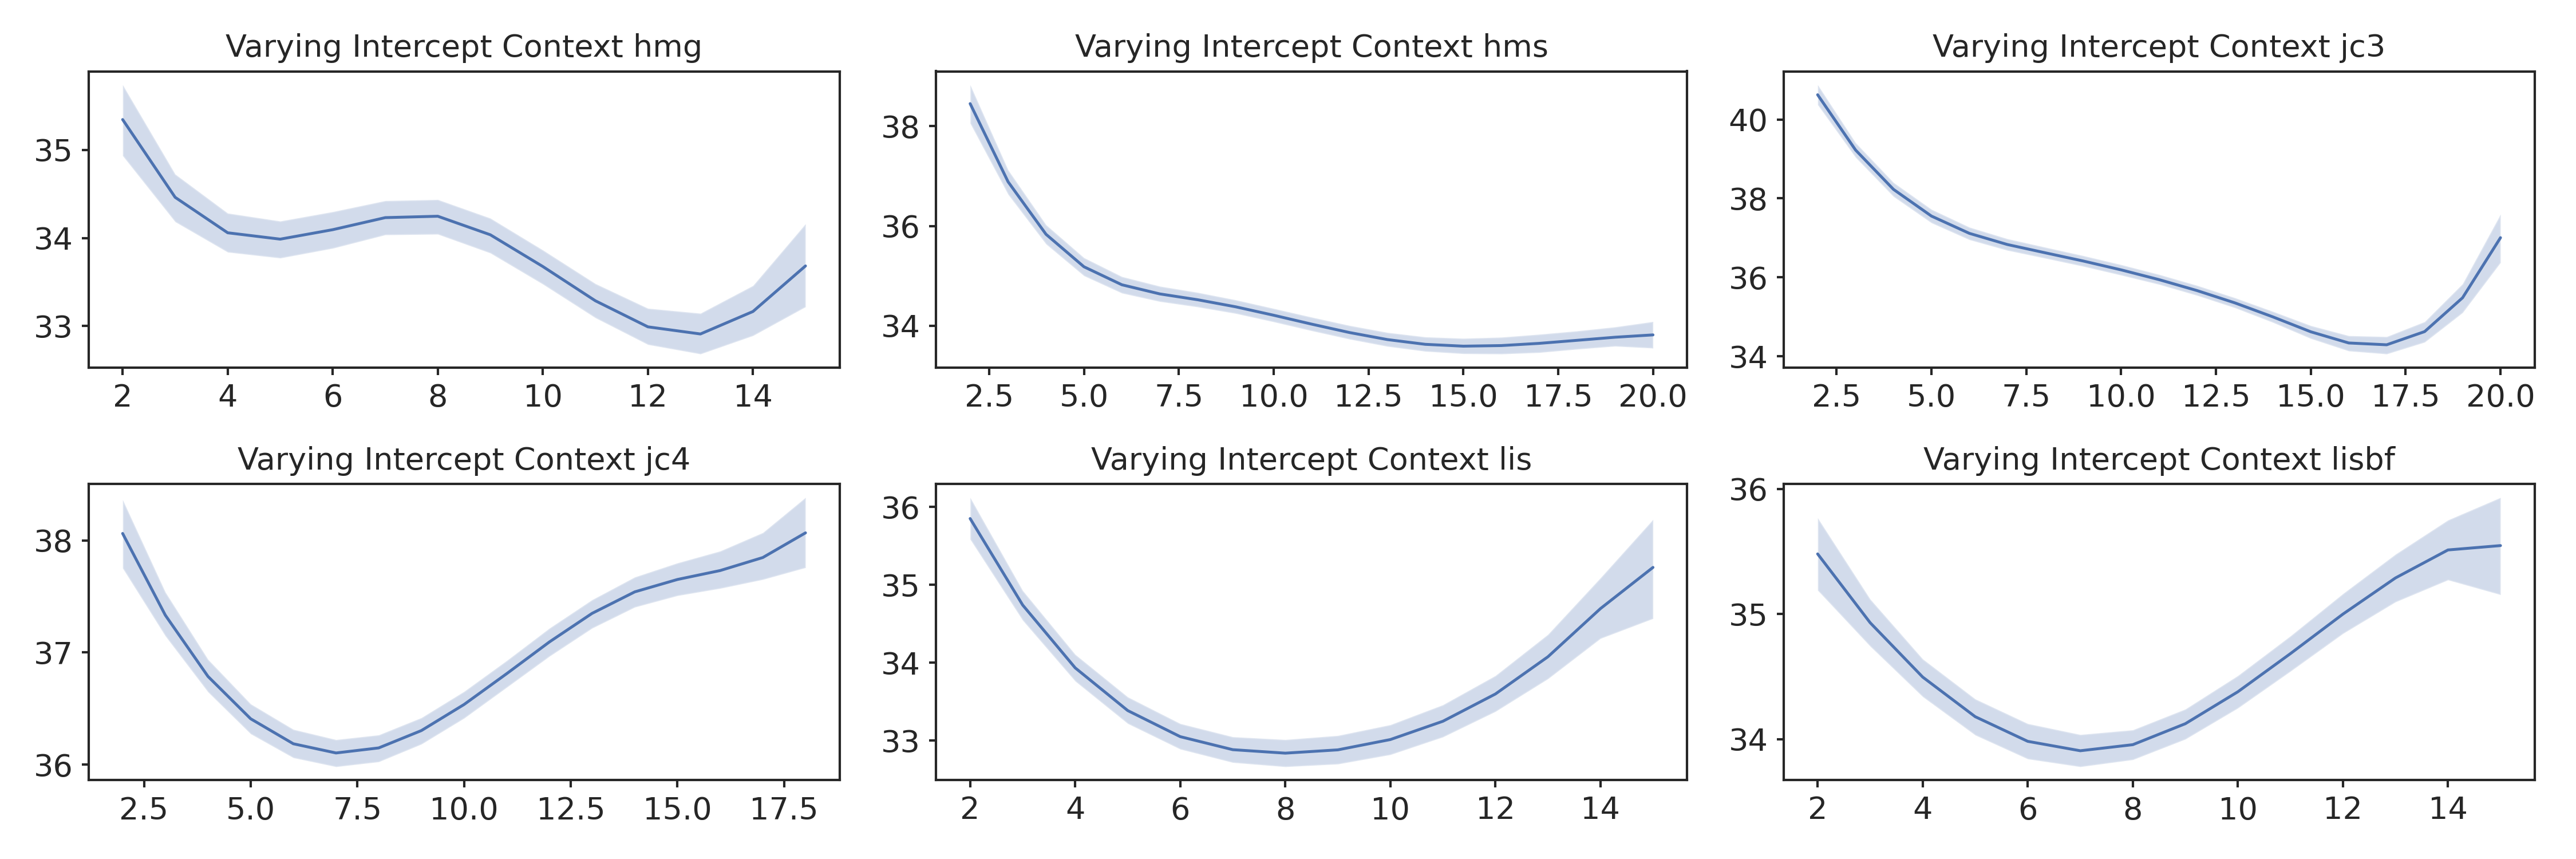
\includegraphics[width=\textwidth]{images/appendix_C/collapsed_interc_2.png}
\caption[\textbf{Targets collapsed time-varying random intercept}]{Time varying random intercept estimated by the model fitted for the Future Absence target.}
\label{interc_coll_2}
\end{figure}
\FloatBarrier

\begin{figure}[ht]
\centering
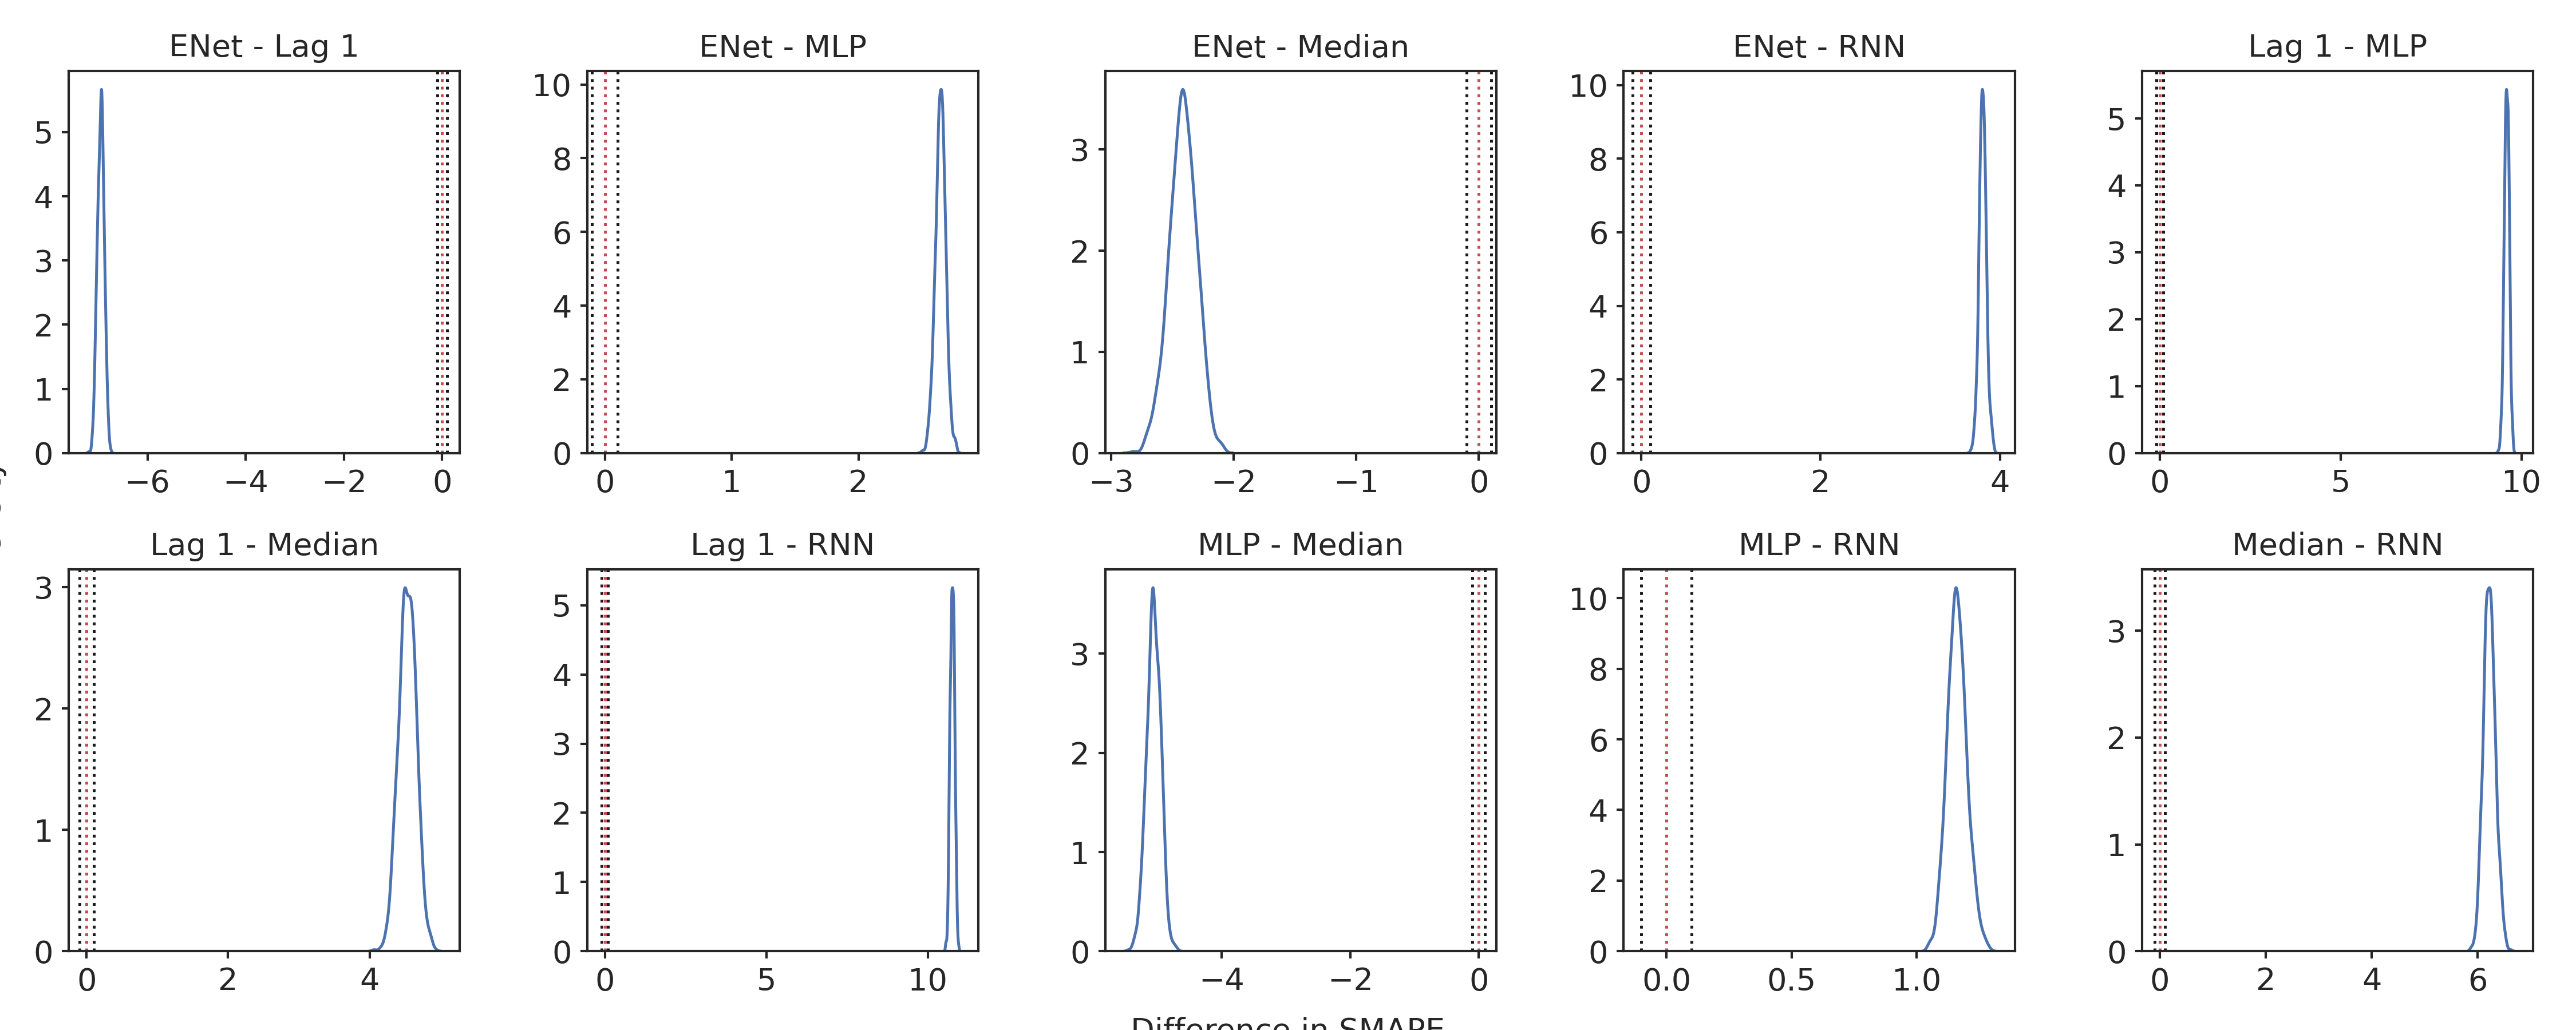
\includegraphics[width=\textwidth]{images/appendix_C/collapsed_comp_2.png}
\caption[\textbf{Targets collapsed pairwise comparisons of model fixed effect}]{Pairwise comparisons of the parameter $\alpha$ (i.e. model slope) estimated by the model fitted for the Future Absence target.}
\label{comp_coll_2}
\end{figure}
\FloatBarrier

\subsection{Future Absence}
\label{future_abs_bayes_2}

\begin{figure}[ht]
\centering
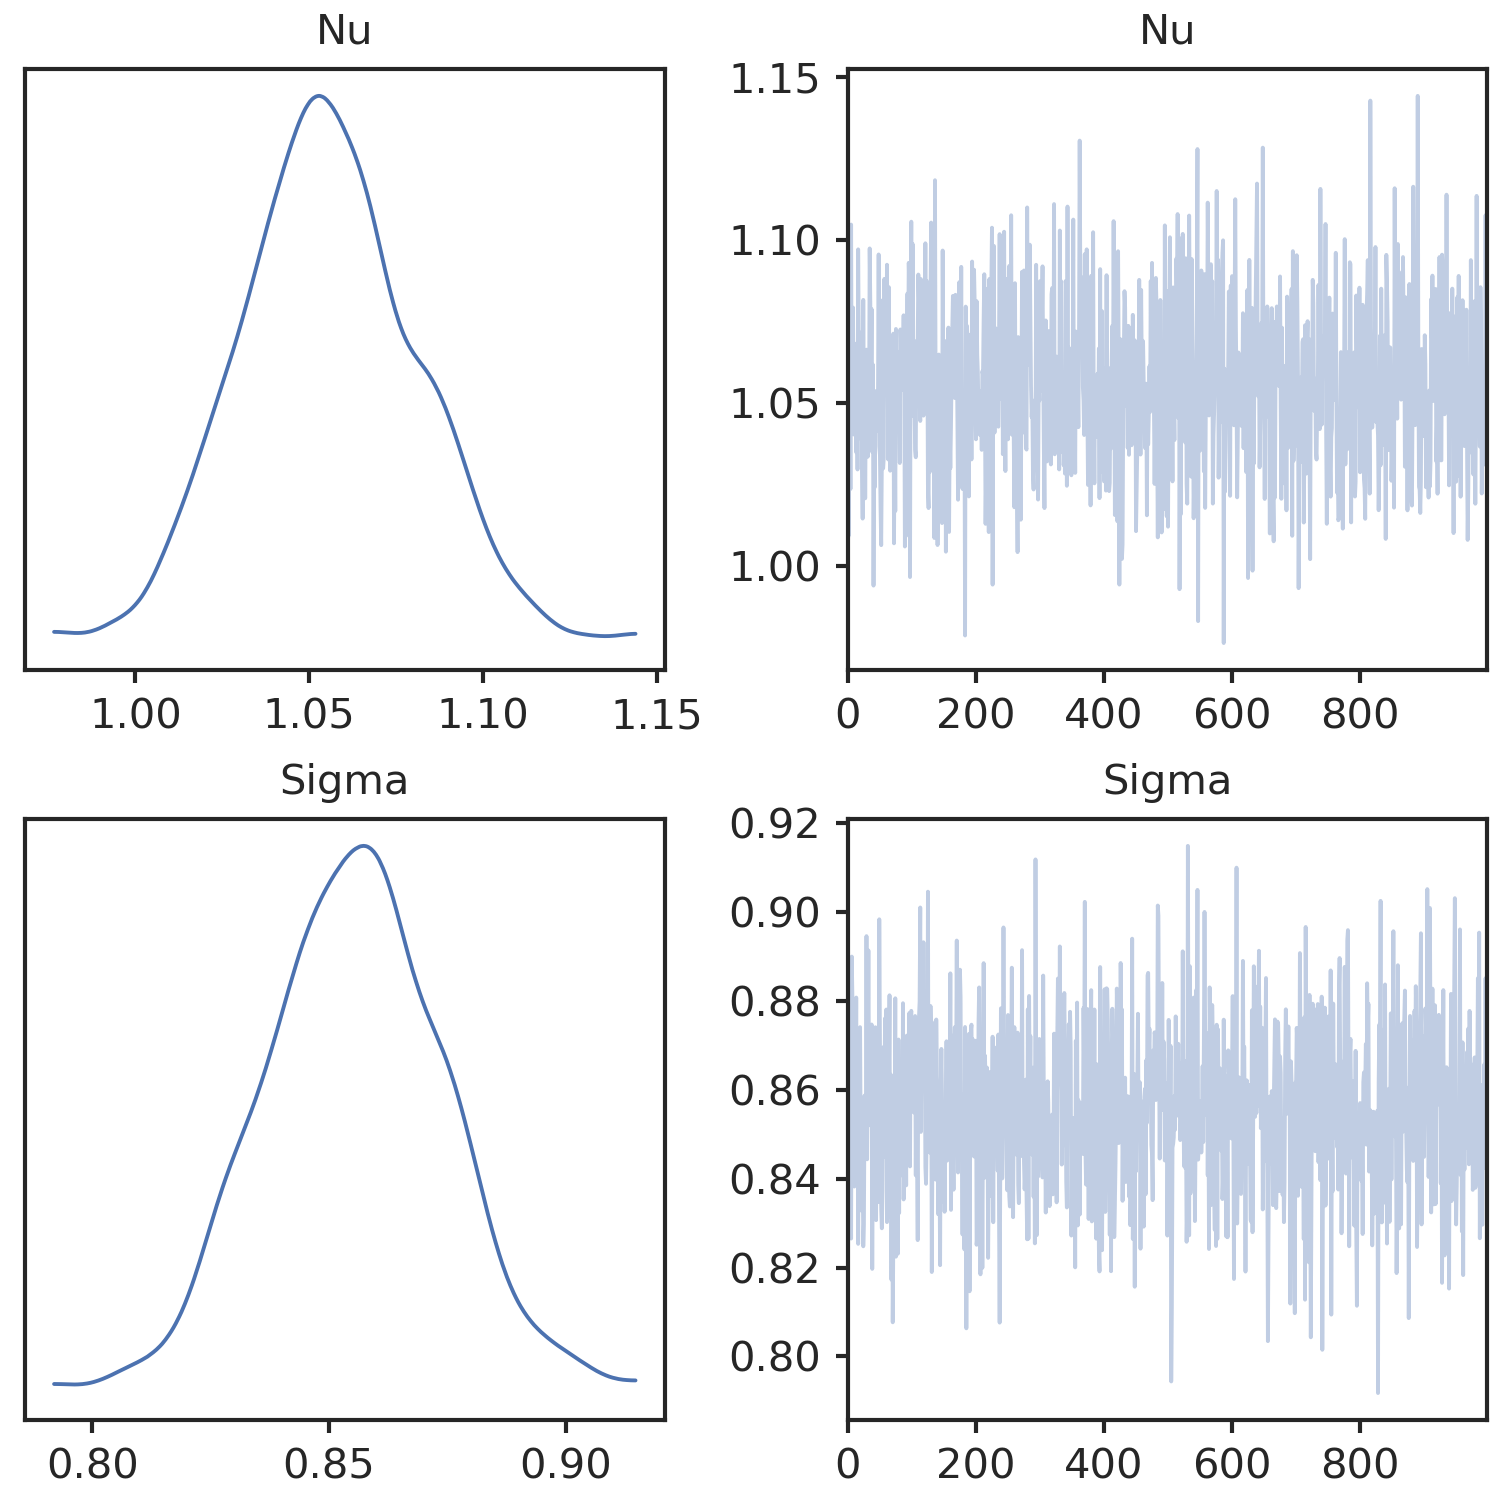
\includegraphics[width=0.5\textwidth]{images/appendix_C/Future Absence_marginals_2.png}
\caption[\textbf{Future absence marginal distributions}]{Marginal distributions for the parameters $\nu$, $\sigma$ estimated by the model fitted for the Future Absence target.}
\label{marginals_abs_2}
\end{figure}
\FloatBarrier

\begin{figure}[ht]
\centering
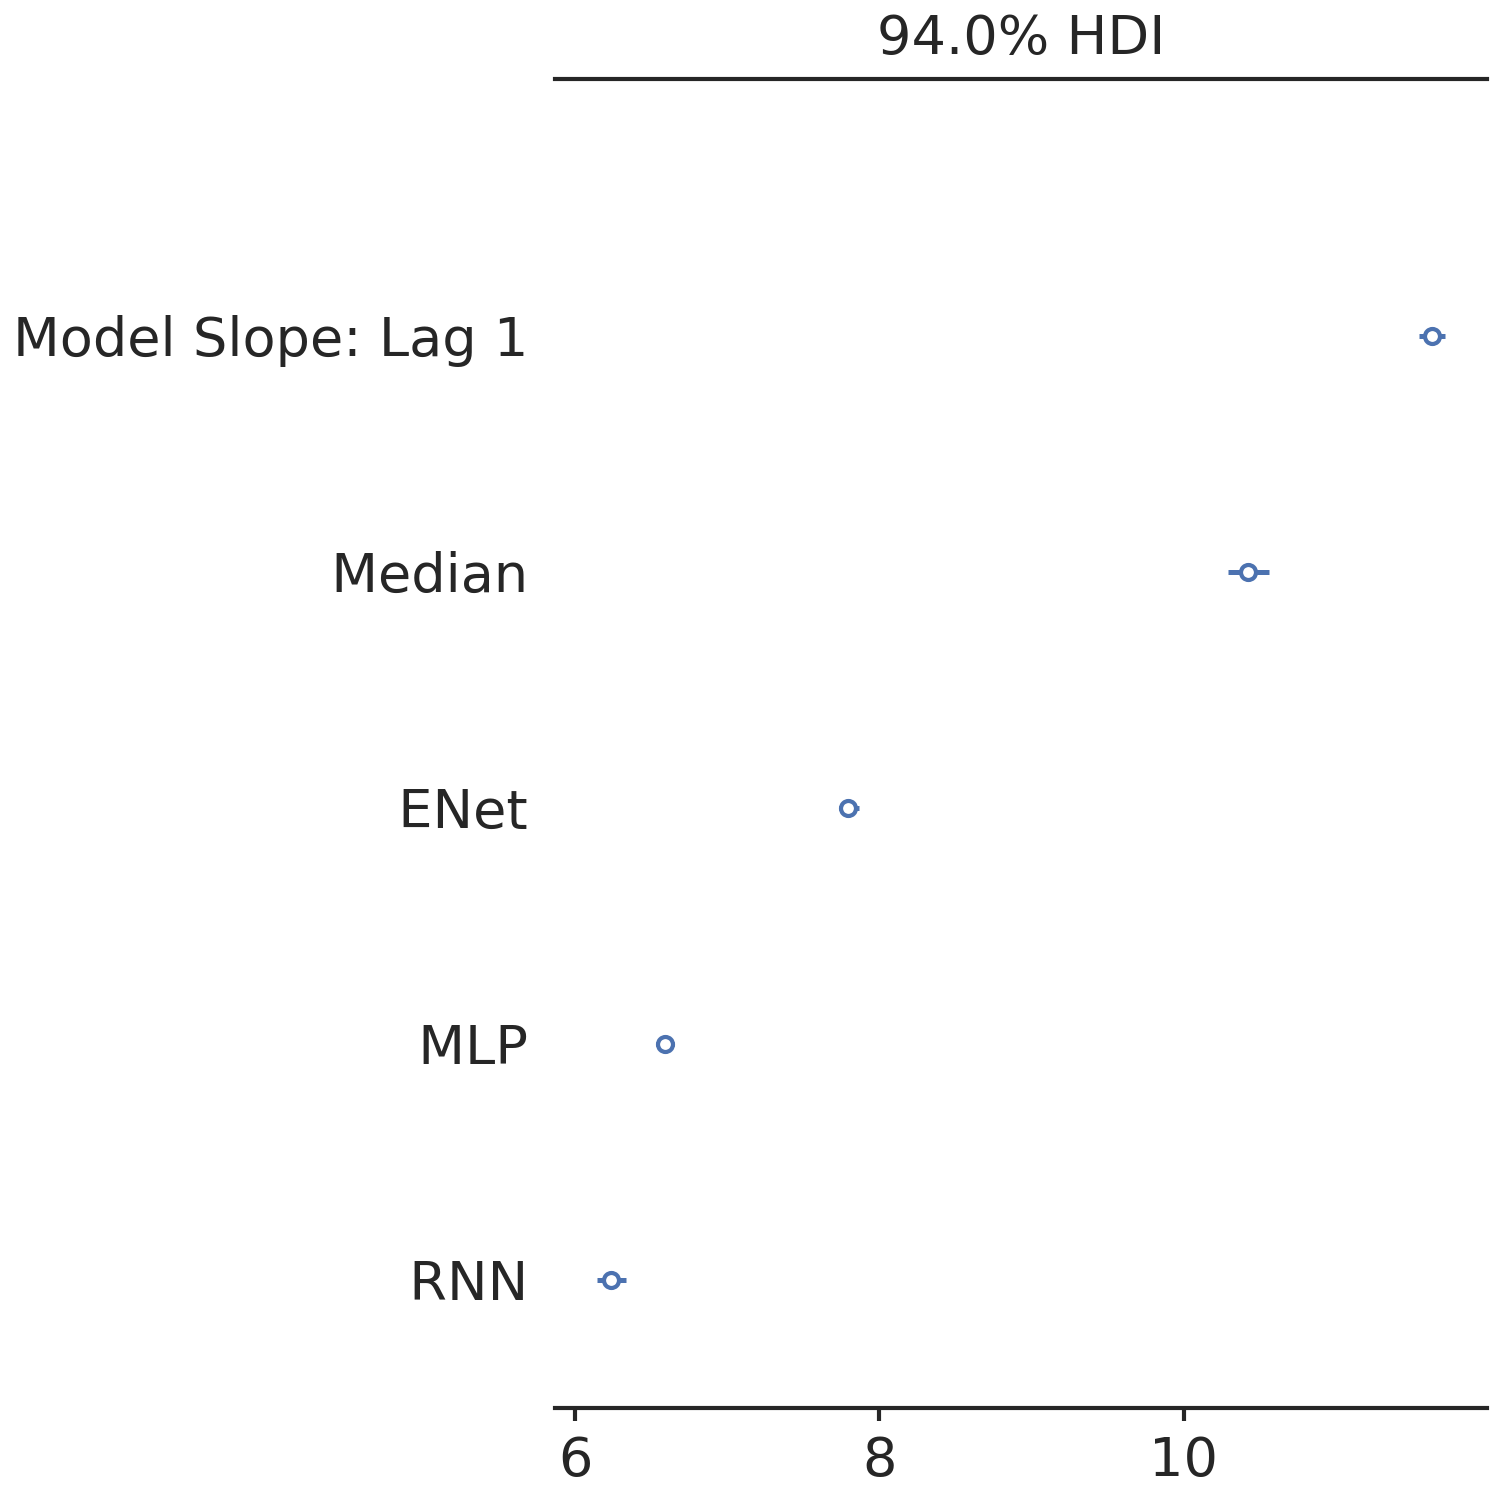
\includegraphics[width=0.5\textwidth]{images/appendix_C/Future Absence_models_2.png}
\caption[\textbf{Future absence model fixed effect}]{Forest plot of the marginal distributions for the parameter $\alpha$ (i.e. model slope) estimated by the model fitted for the Future Absence target.}
\label{model_abs_2}
\end{figure}
\FloatBarrier

\begin{figure}[ht]
\centering
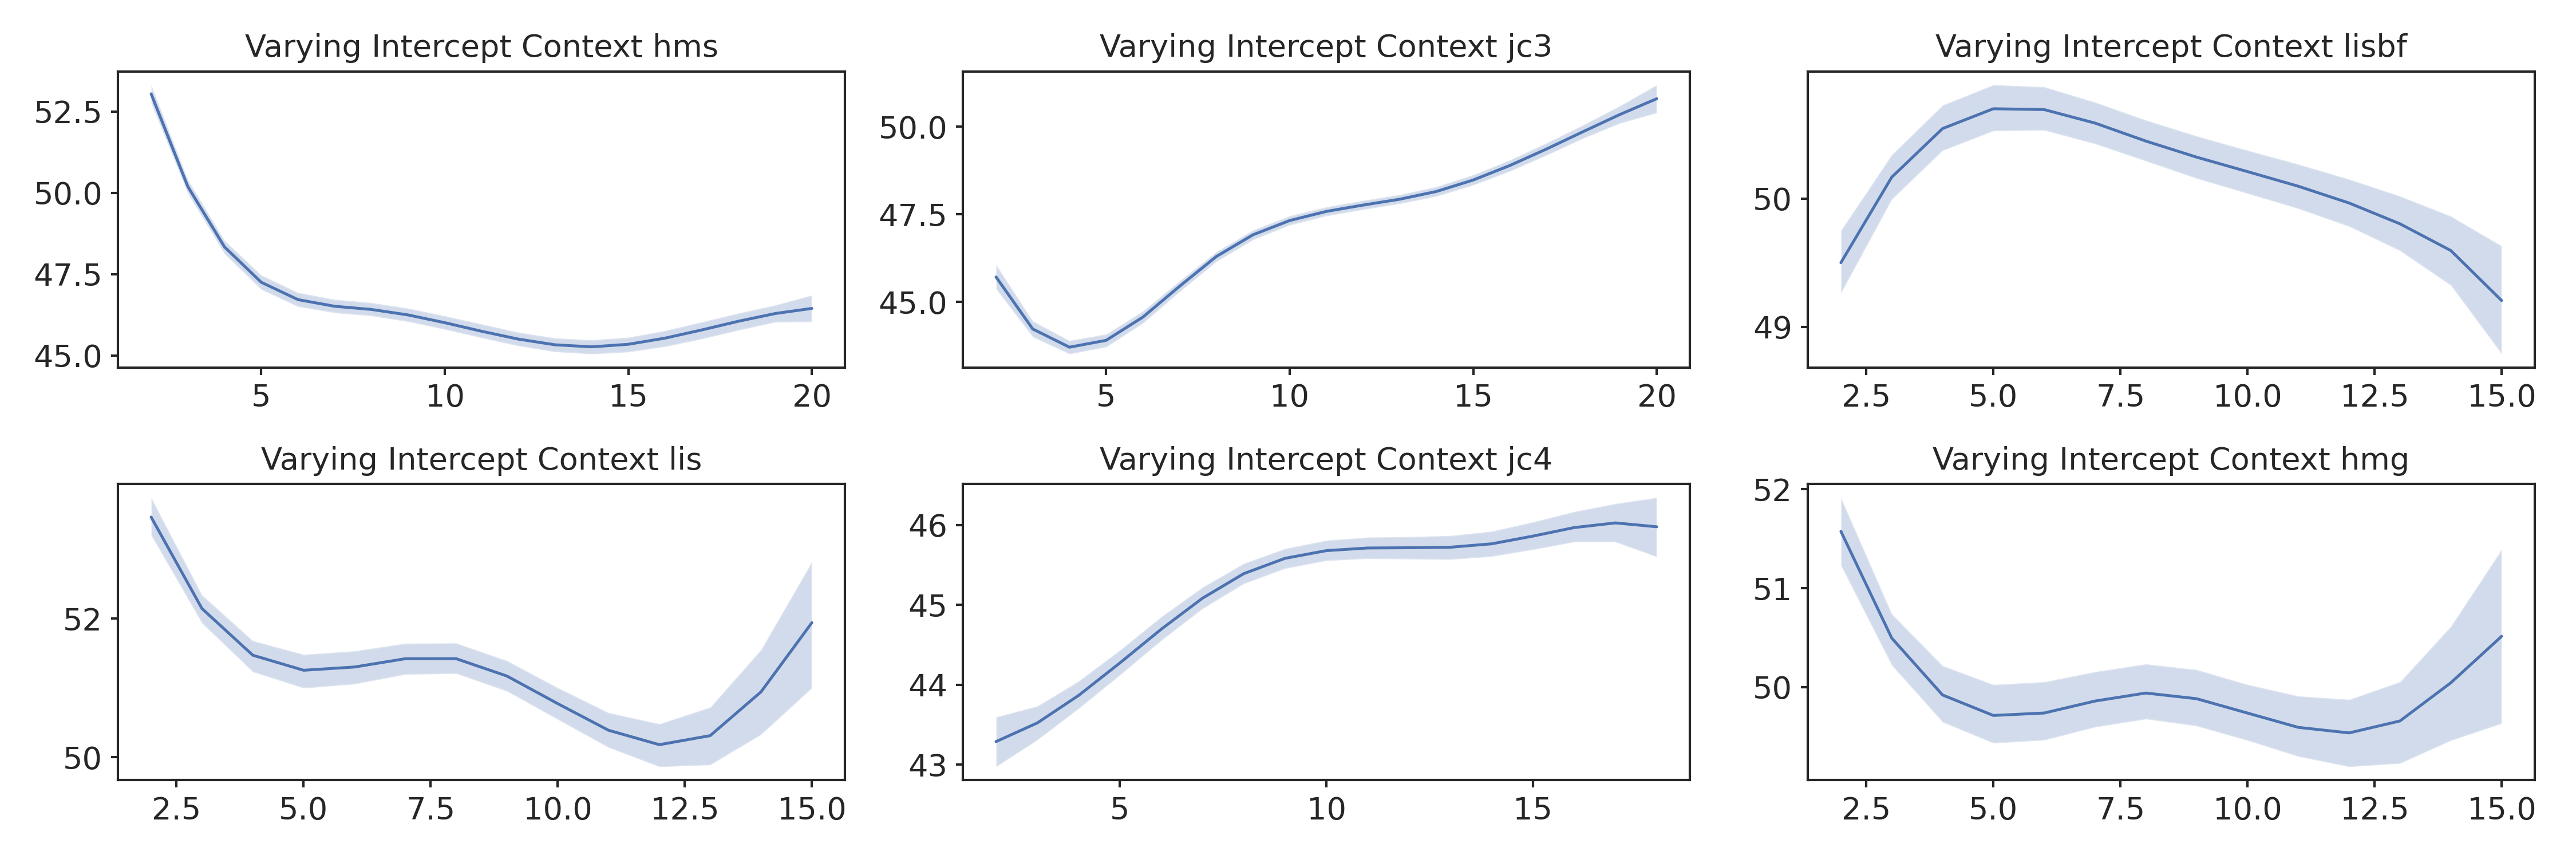
\includegraphics[width=\textwidth]{images/appendix_C/Future Absence_interc_2.png}
\caption[\textbf{Future absence time-varying random intercept}]{Time varying random intercept estimated by the model fitted for the Future Absence target.}
\label{interc_abs_2}
\end{figure}
\FloatBarrier

\begin{figure}[ht]
\centering
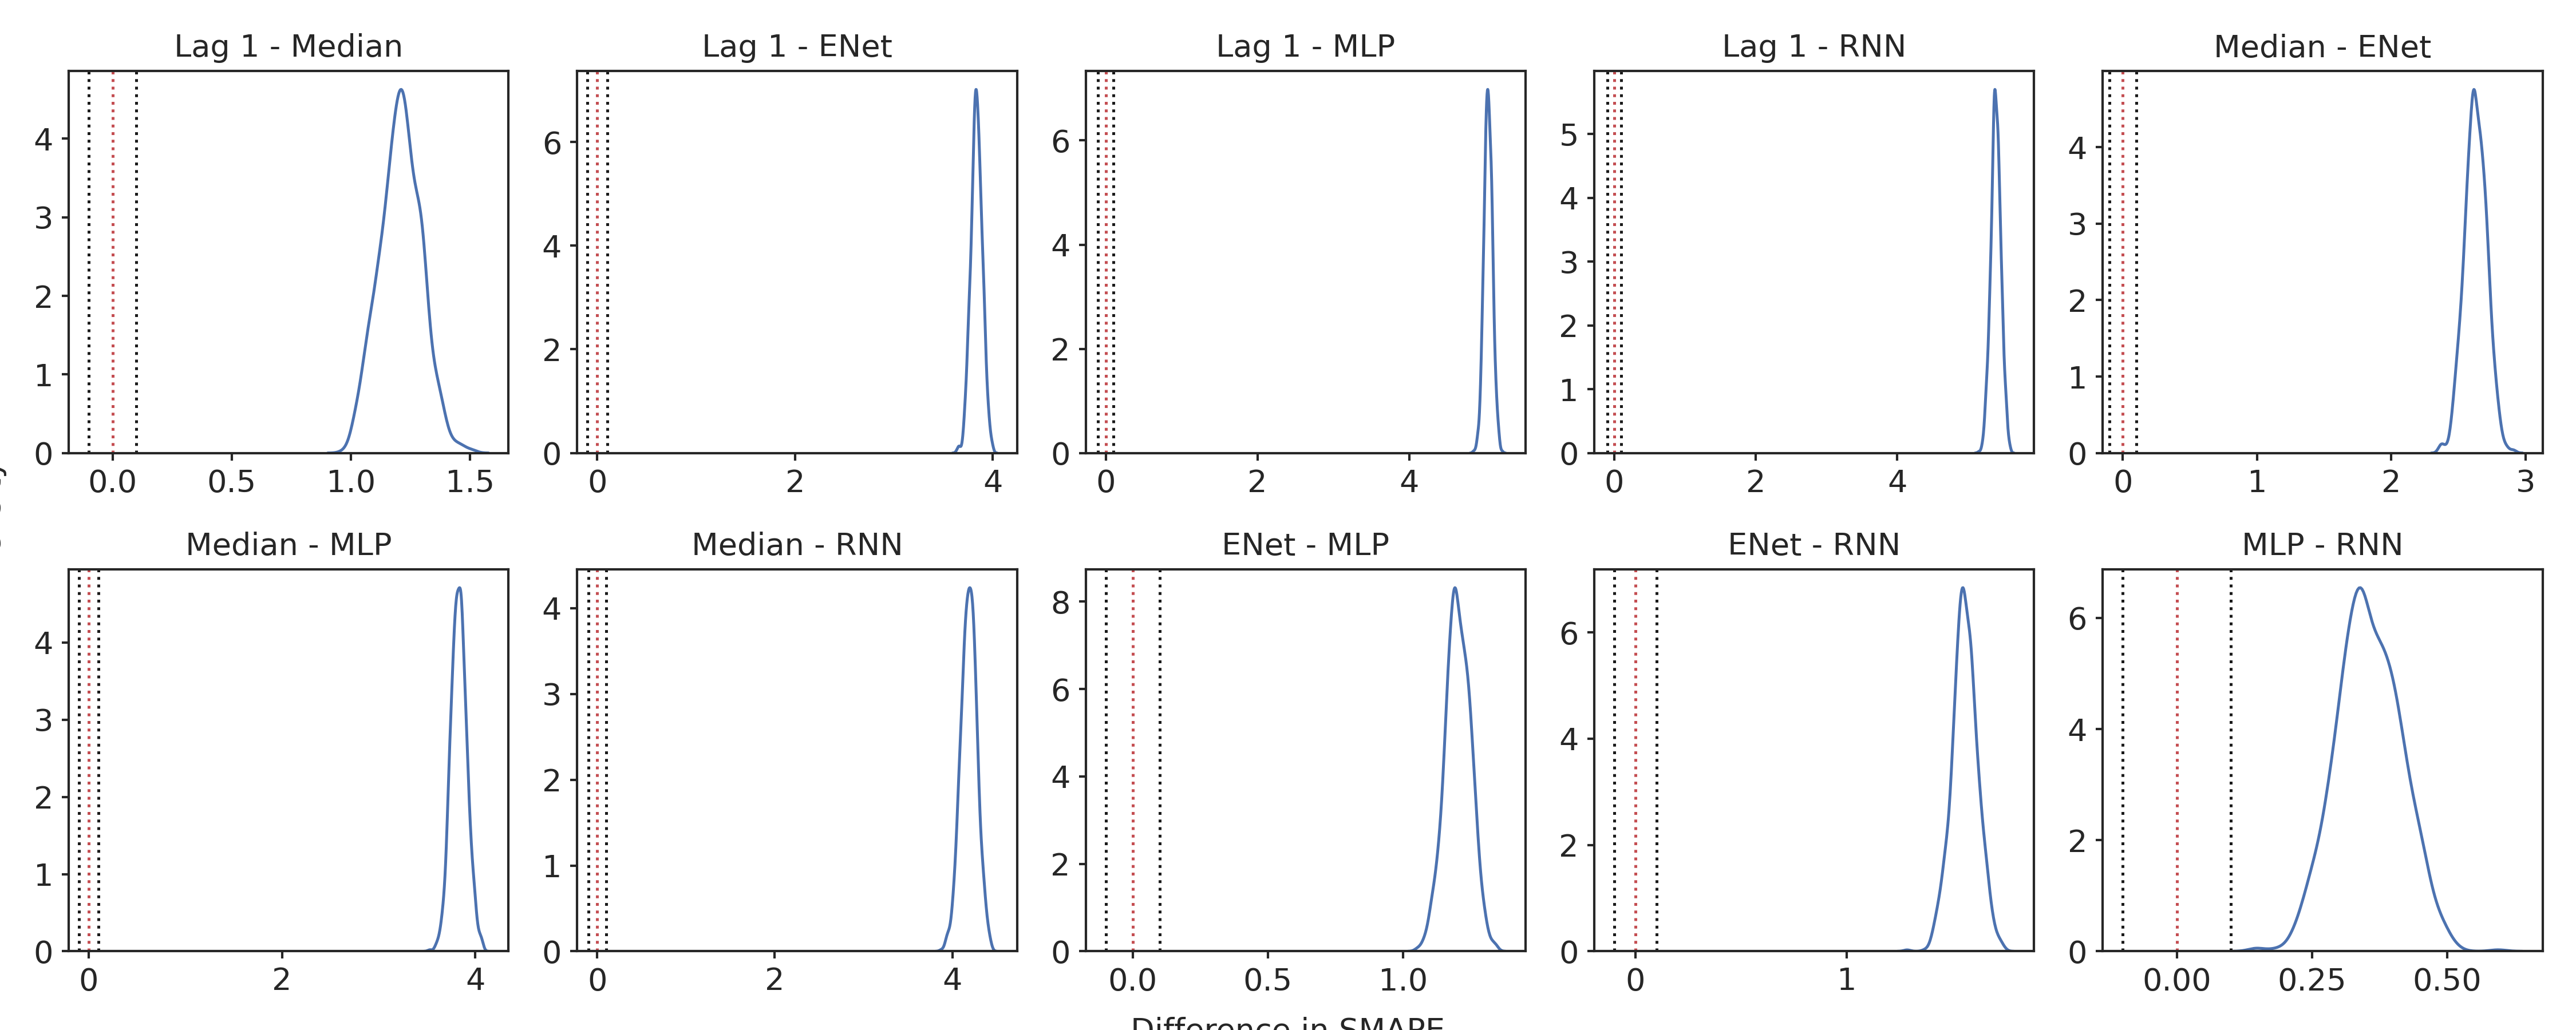
\includegraphics[width=\textwidth]{images/appendix_C/Future_Absence_comp_2.png}
\caption[\textbf{Future absence pairwise comparisons of model fixed effect}]{Pairwise comparisons of the parameter $\alpha$ (i.e. model slope) estimated by the model fitted for the Future Absence target.}
\label{comp_abs_2}
\end{figure}
\FloatBarrier

\subsection{Future Active Time}
\label{future_abs_bayes_2}

\begin{figure}[ht]
\centering
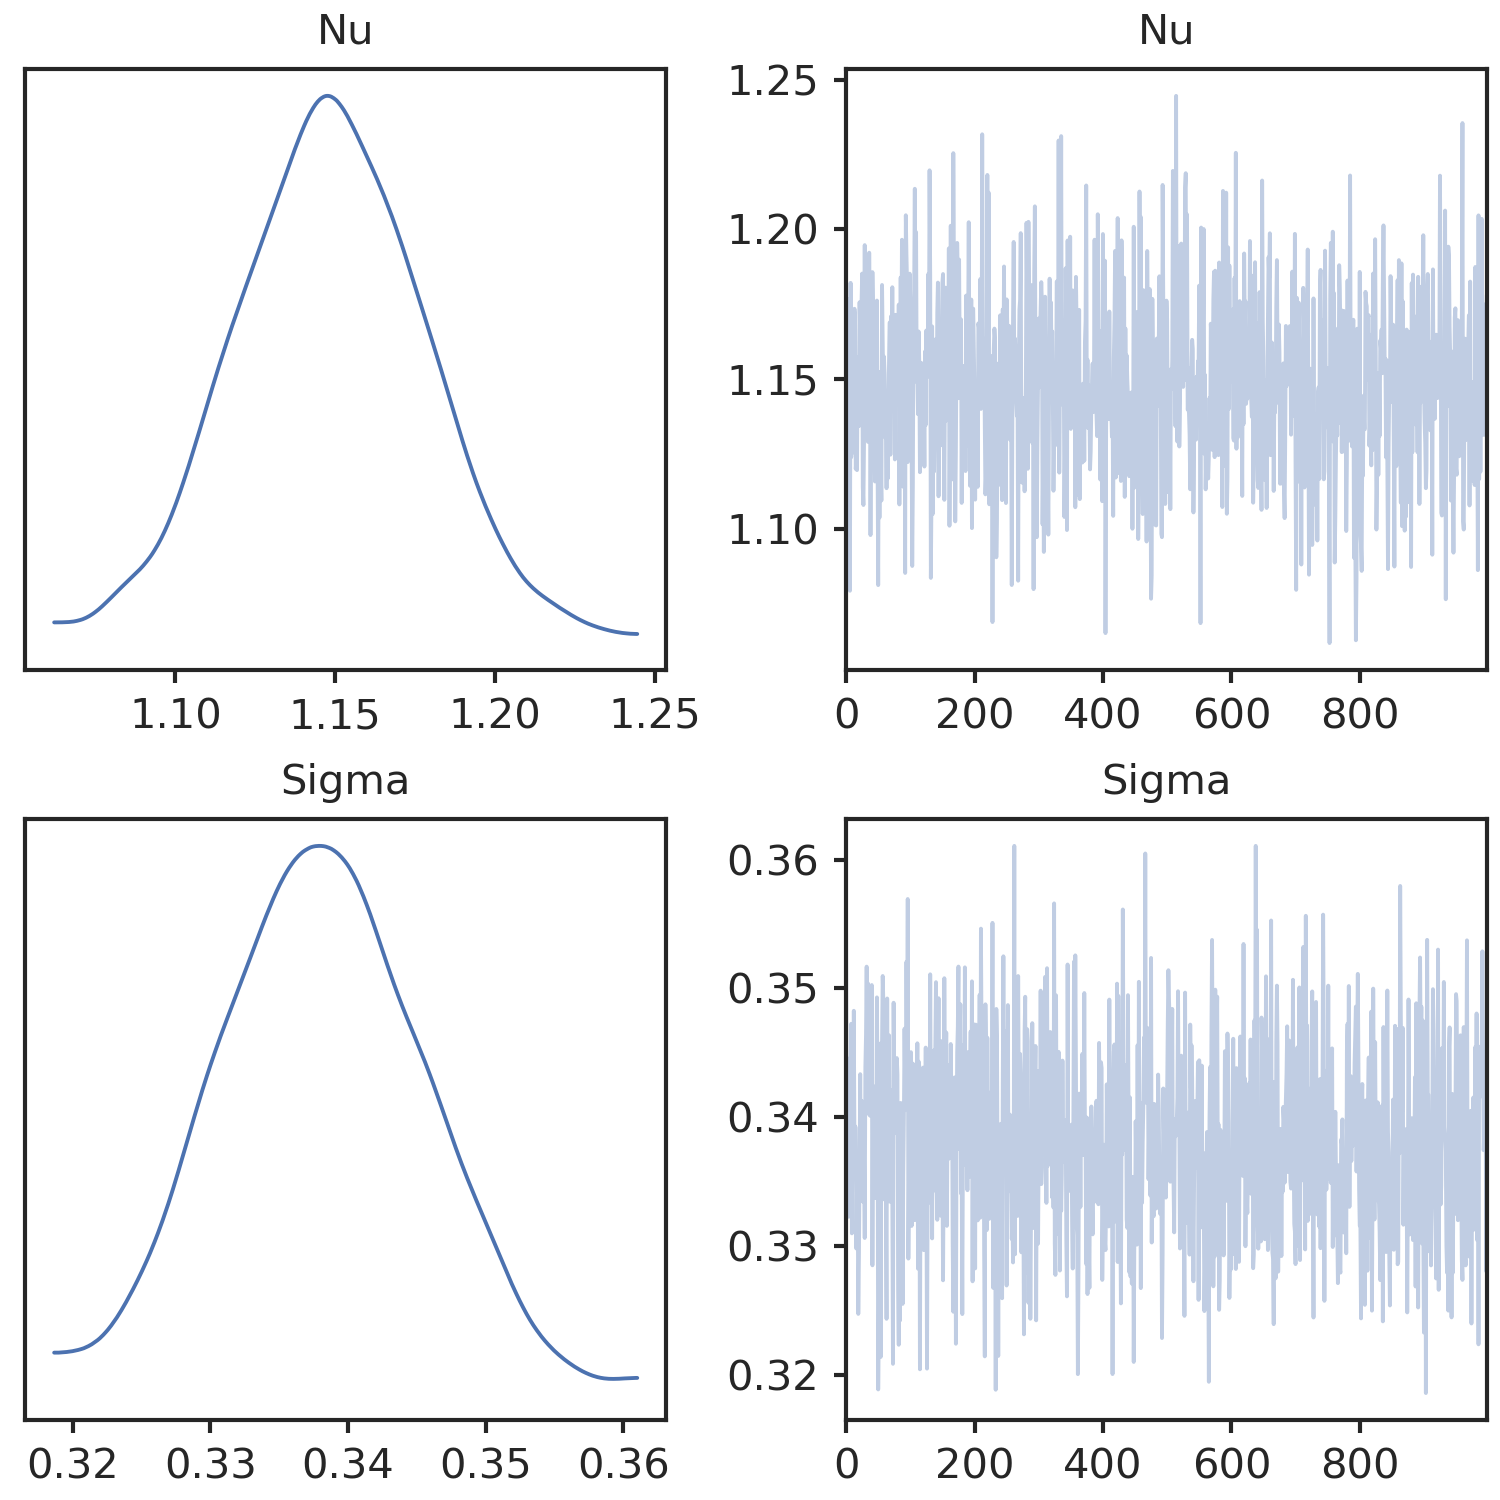
\includegraphics[width=0.5\textwidth]{images/appendix_C/Future Active Time_marginals_2.png}
\caption[\textbf{Future active time marginal distributions}]{Marginal distributions for the parameters $\nu$, $\sigma$ estimated by the model fitted for the Future Active Time target.}
\label{marginals_act_2}
\end{figure}
\FloatBarrier

\begin{figure}[ht]
\centering
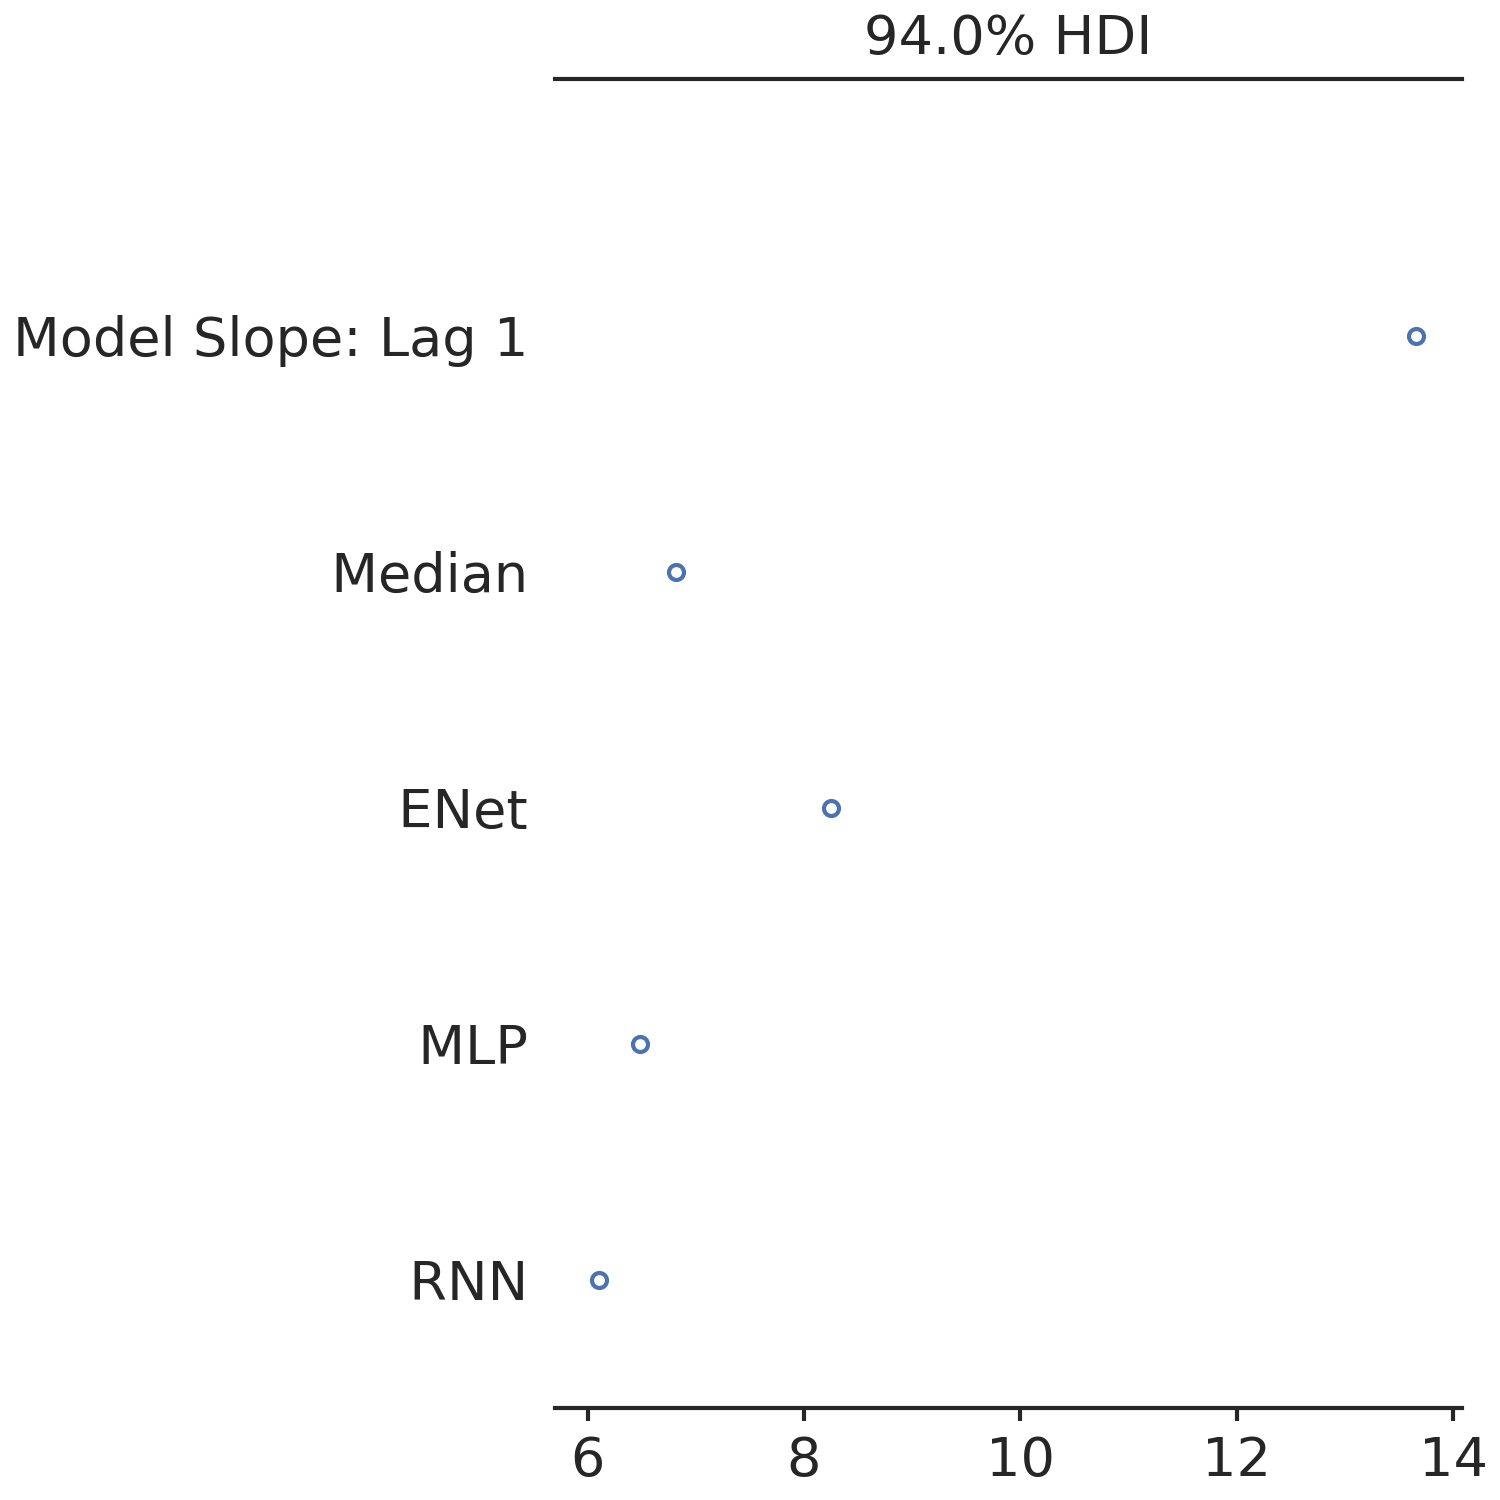
\includegraphics[width=0.5\textwidth]{images/appendix_C/Future Active Time_models_2.png}
\caption[\textbf{Future active time model fixed effect}]{Forest plot of the marginal distributions for the parameter $\alpha$ (i.e. model slope) estimated by the model fitted for the Future Active Time target.}
\label{model_act_2}
\end{figure}
\FloatBarrier

\begin{figure}[ht]
\centering
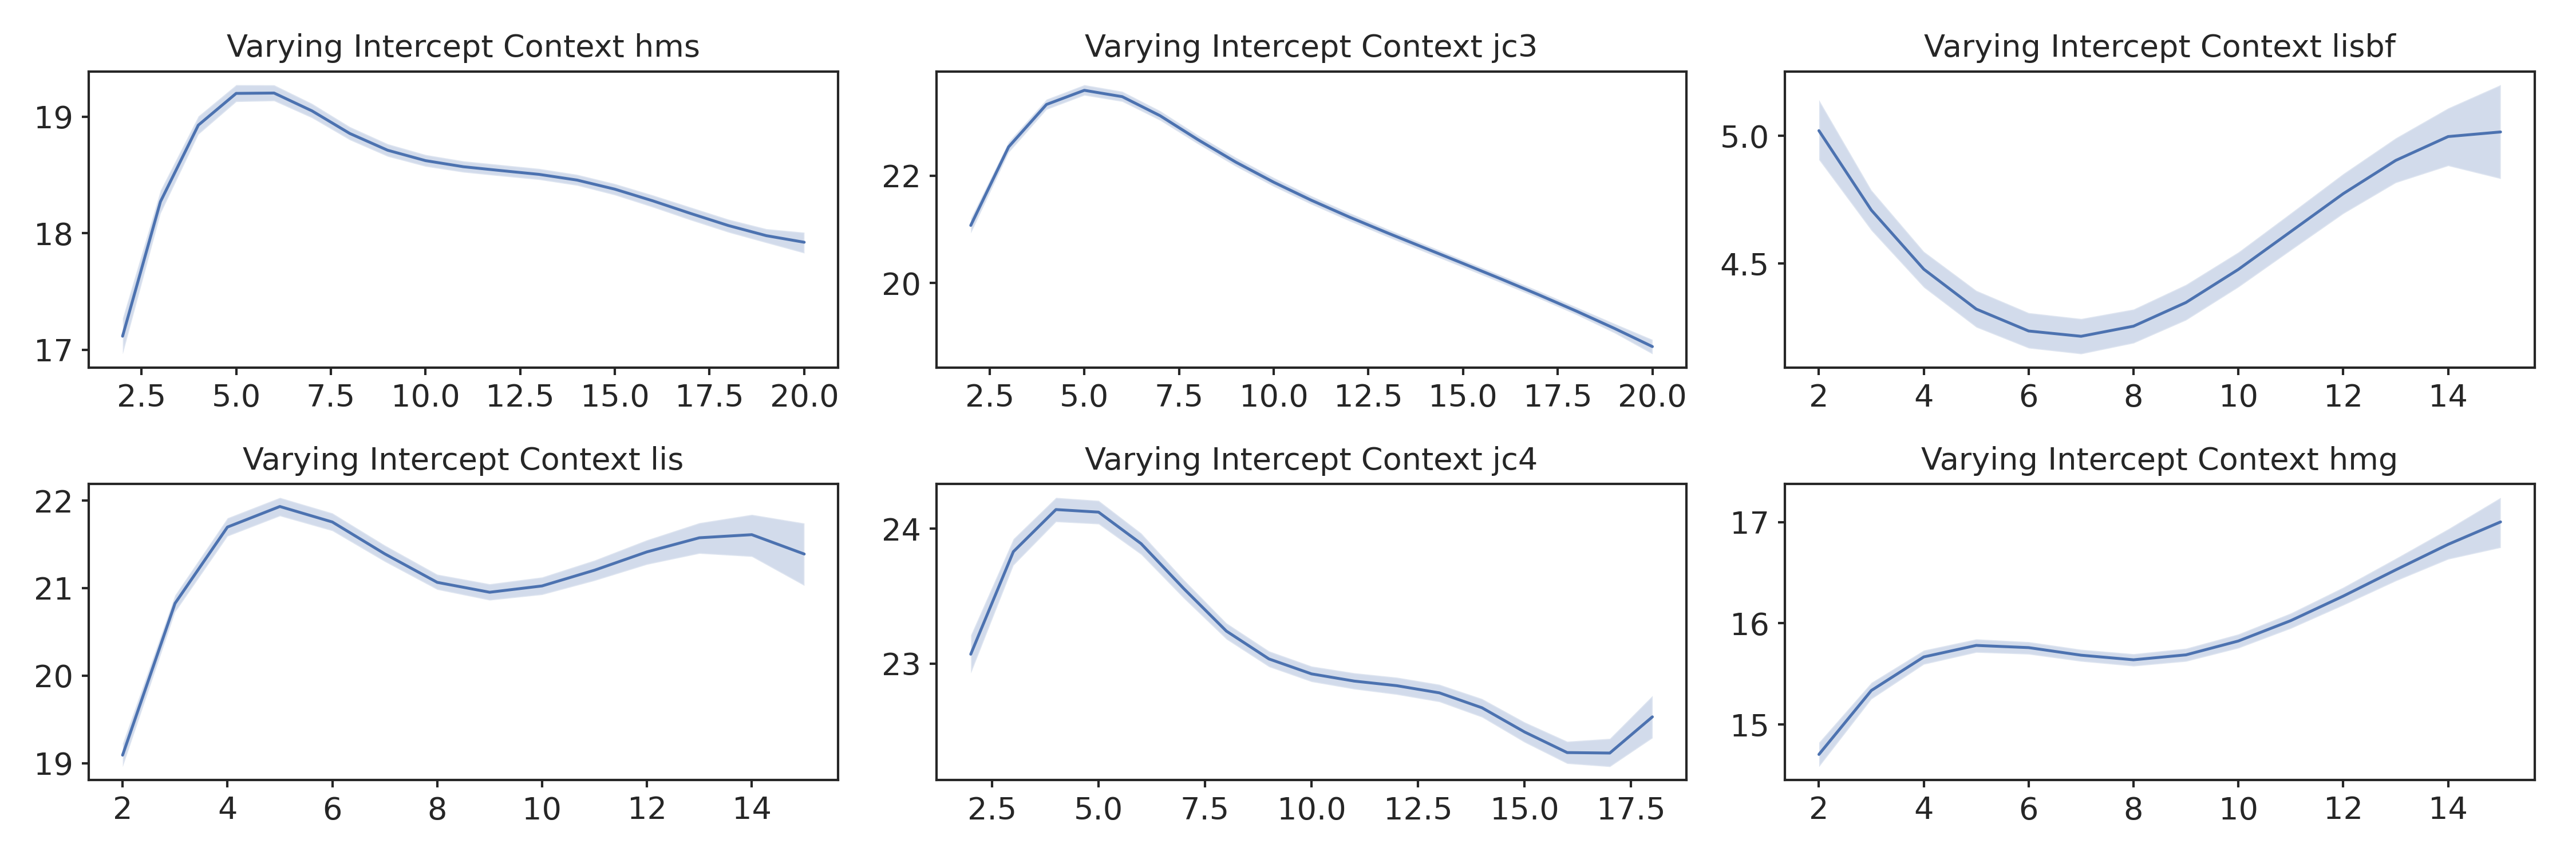
\includegraphics[width=\textwidth]{images/appendix_C/Future Active Time_interc_2.png}
\caption[\textbf{Future active time time-varying random intercept}]{Time varying random intercept estimated by the model fitted for the Future Active Time target.}
\label{interc_act_2}
\end{figure}
\FloatBarrier

\begin{figure}[ht]
\centering
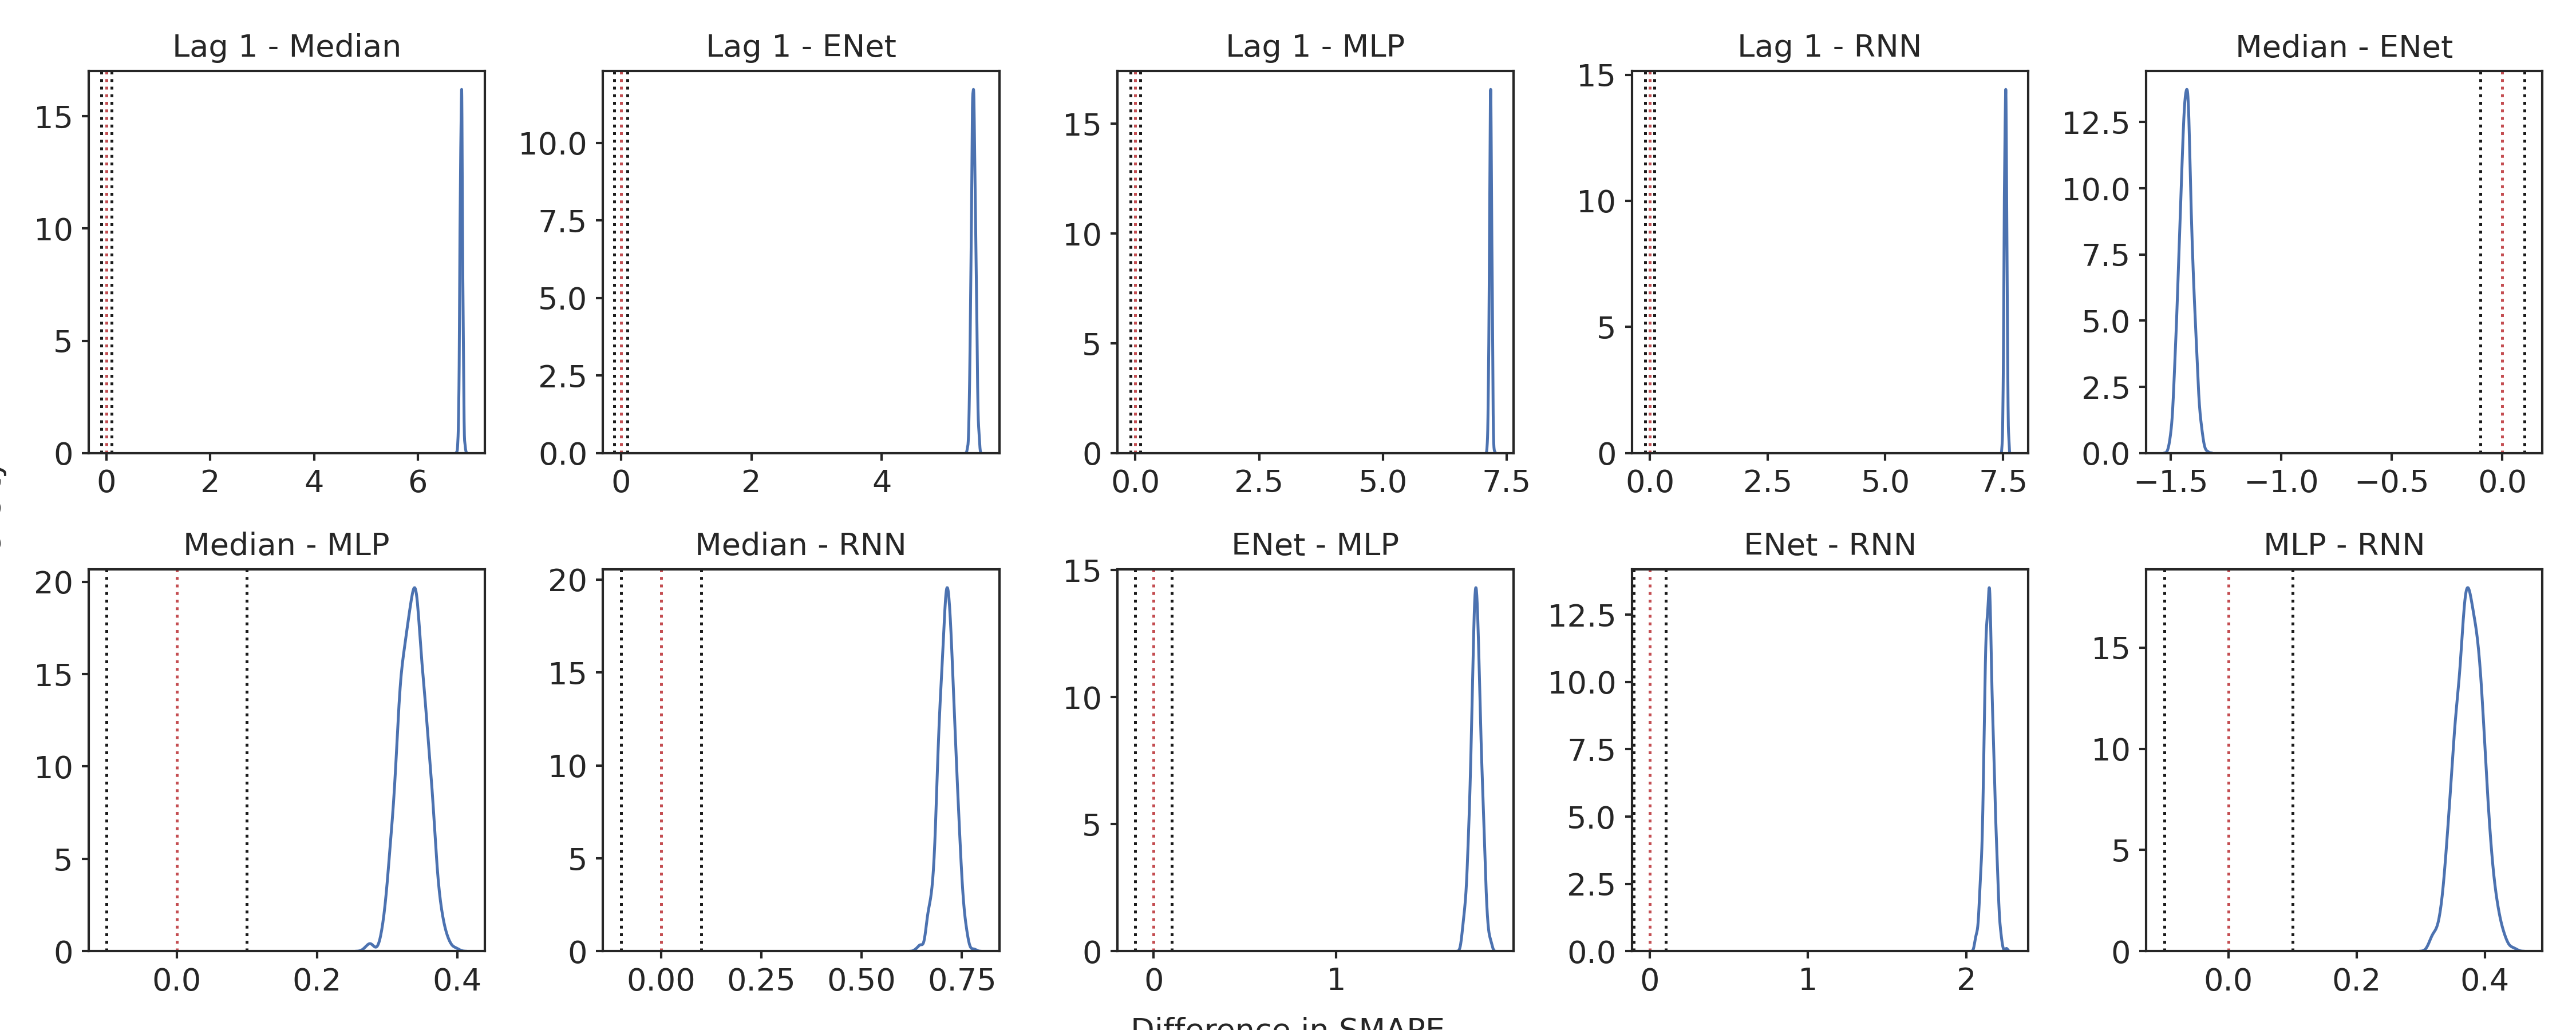
\includegraphics[width=\textwidth]{images/appendix_C/Future_Active_Time_comp_2.png}
\caption[\textbf{Future active time pairwise comparisons of model fixed effect}]{Pairwise comparisons of the parameter $\alpha$ (i.e. model slope) estimated by the model fitted for the Future Active Time target.}
\label{comp_act_2}
\end{figure}
\FloatBarrier

\subsection{Future Session Time}
\label{future_sess_bayes_2}

\begin{figure}[ht]
\centering
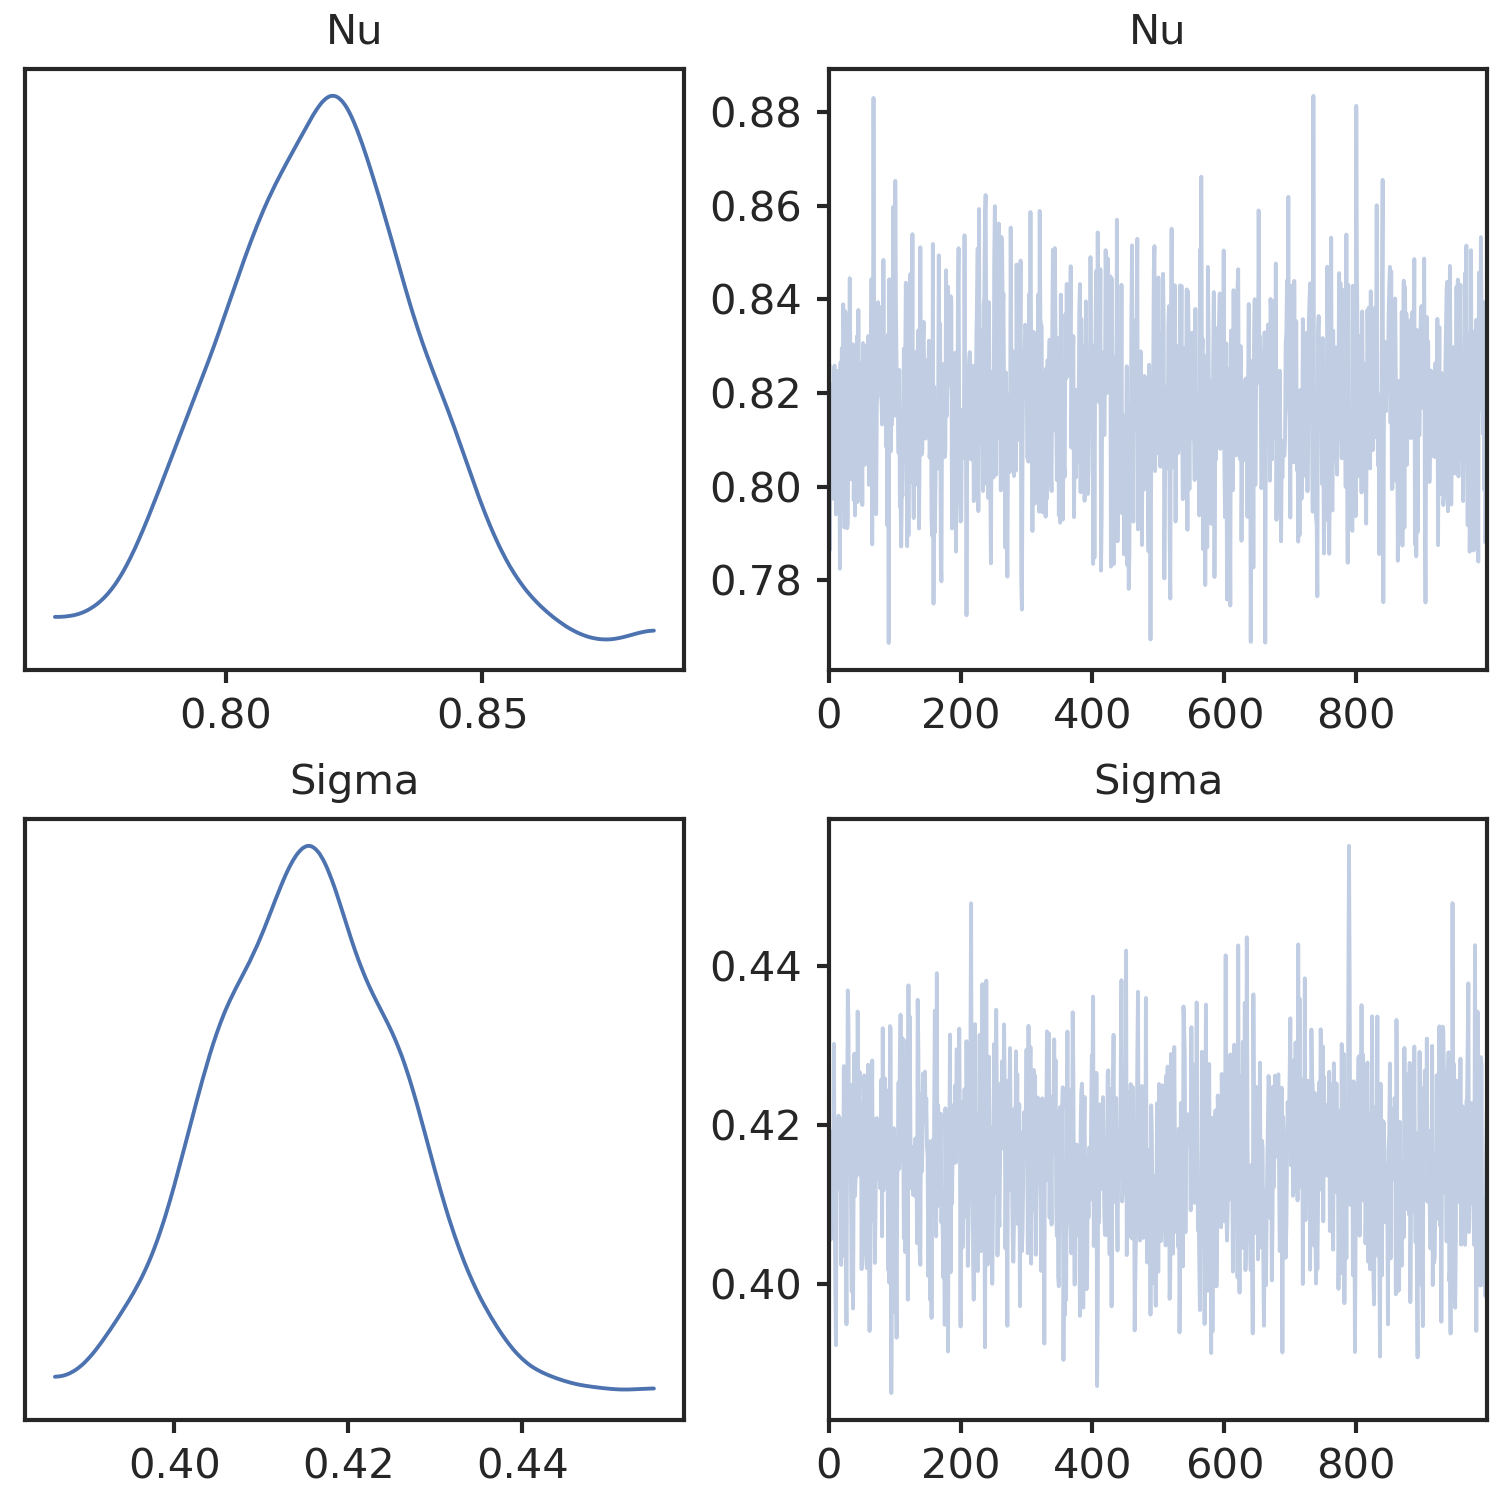
\includegraphics[width=0.5\textwidth]{images/appendix_C/Future Session Time_marginals_2.png}
\caption[\textbf{Future session time marginal distributions}]{Marginal distributions for the parameters $\nu$, $\sigma$ estimated by the model fitted for the Future Session Time target.}
\label{marginals_sess_2}
\end{figure}
\FloatBarrier

\begin{figure}[ht]
\centering
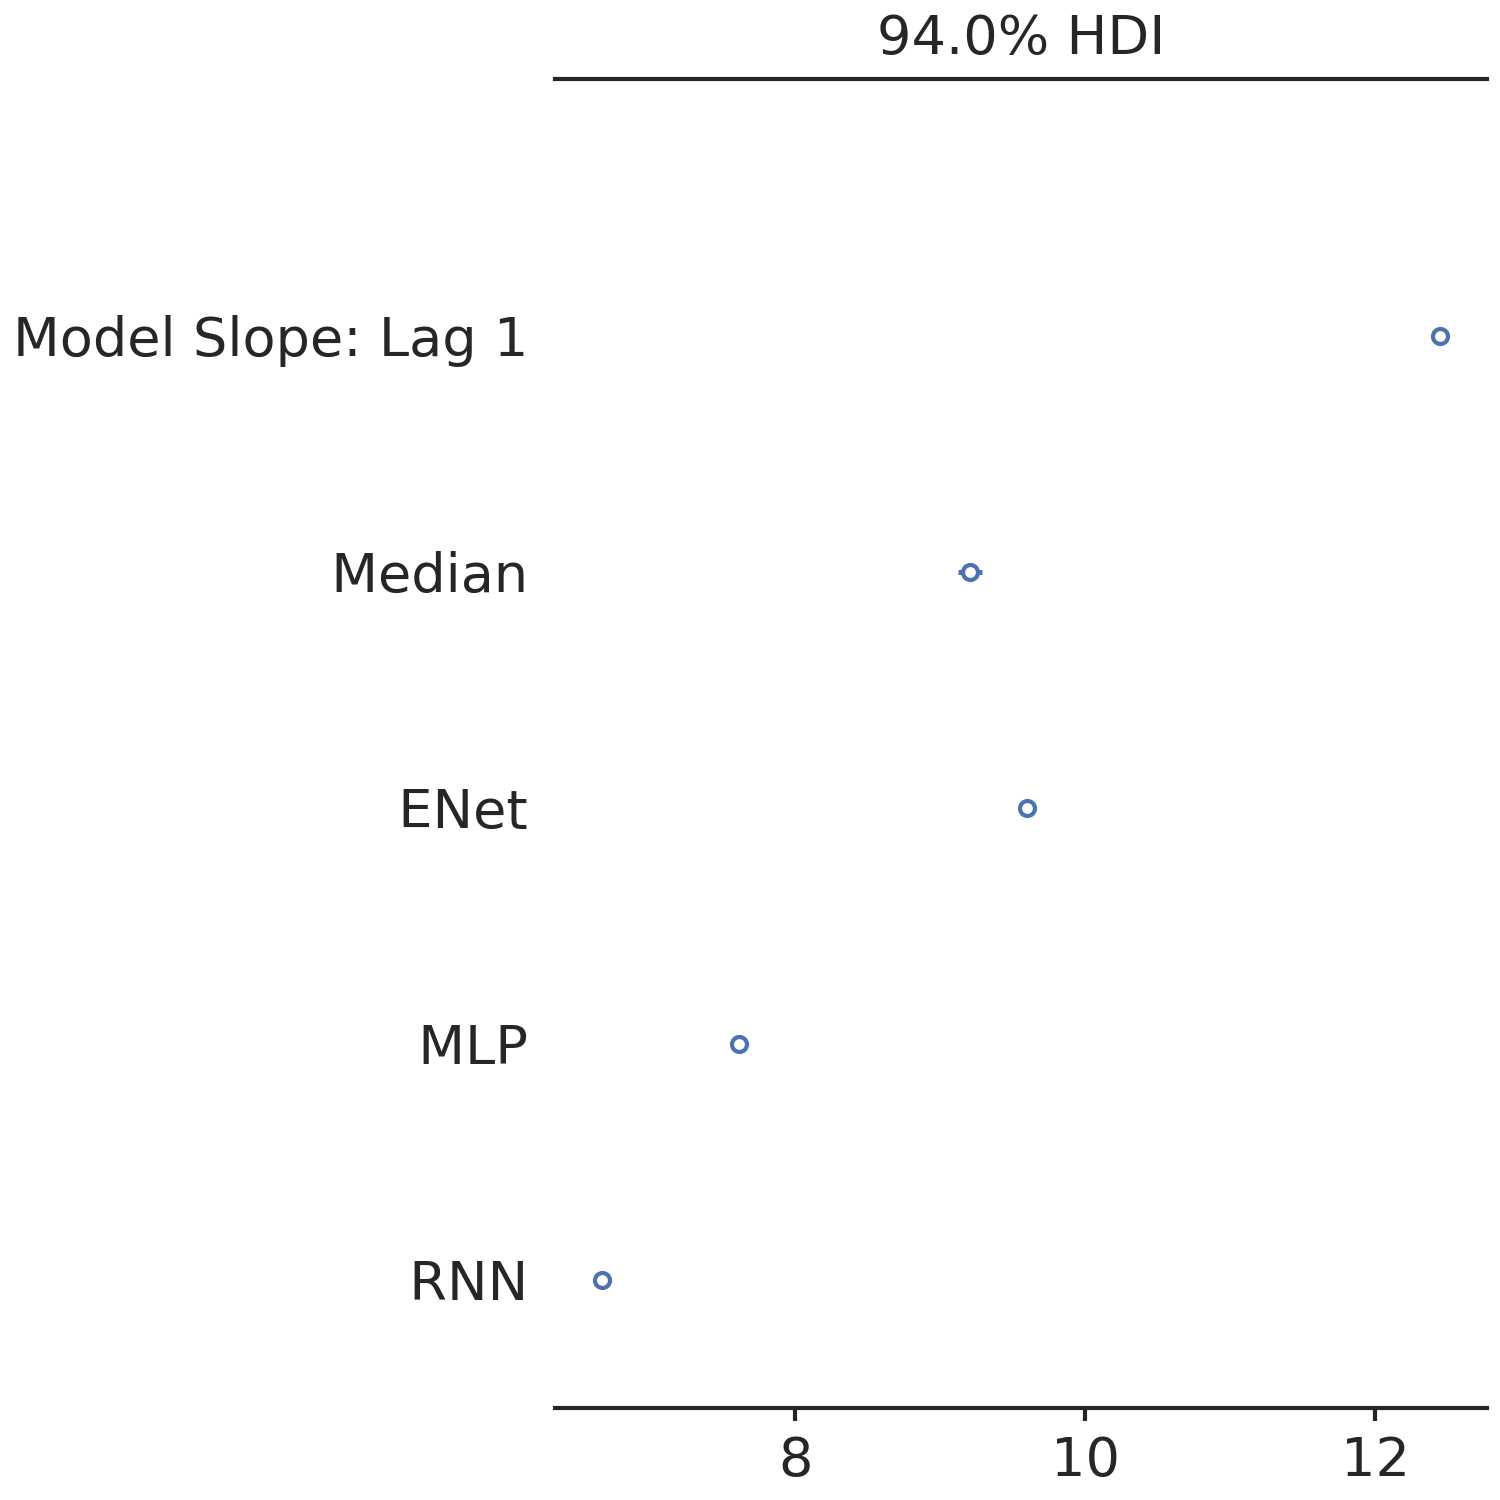
\includegraphics[width=0.5\textwidth]{images/appendix_C/Future Session Time_models_2.png}
\caption[\textbf{Future session time model fixed effect}]{Forest plot of the marginal distributions for the parameter $\alpha$ (i.e. model slope) estimated by the model fitted for the Future Session Time target.}
\label{model_sess_2}
\end{figure}
\FloatBarrier

\begin{figure}[ht]
\centering
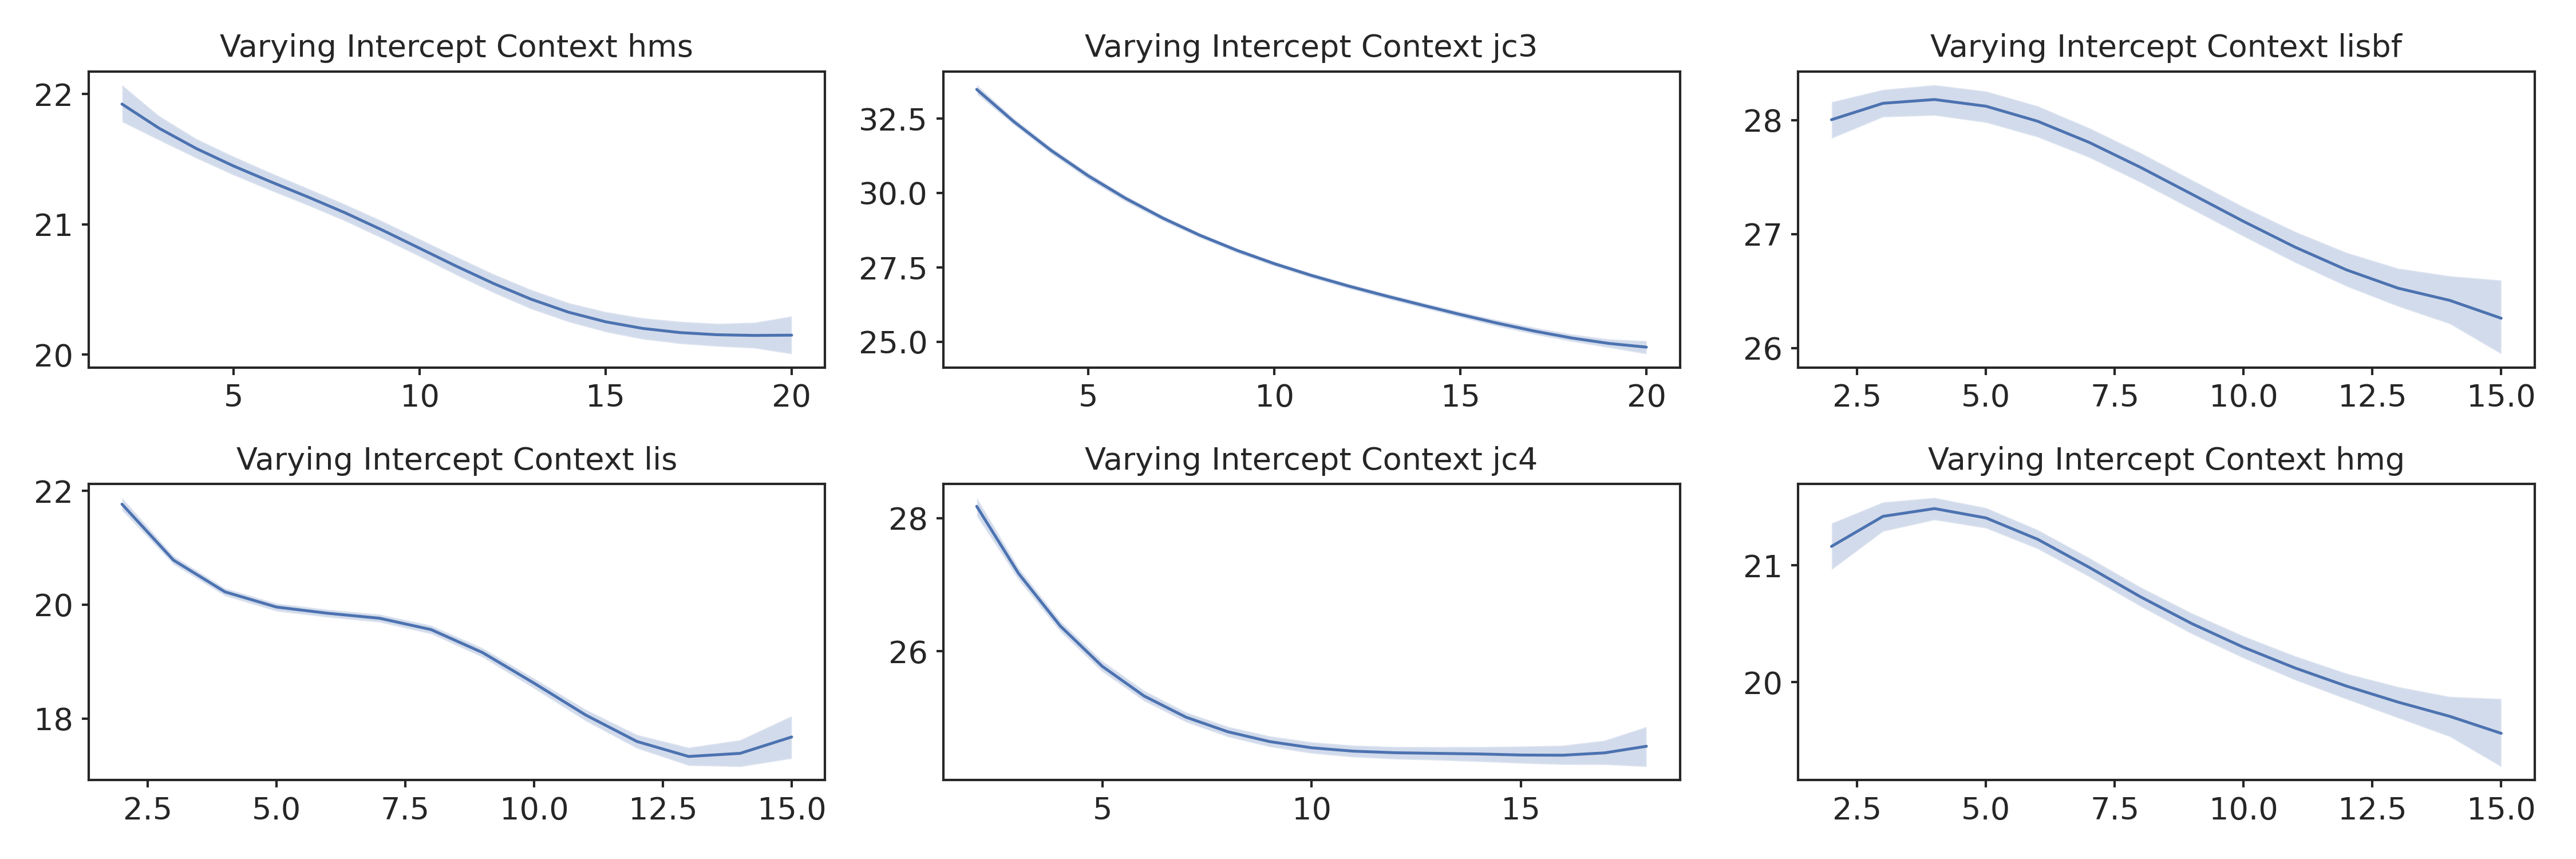
\includegraphics[width=\textwidth]{images/appendix_C/Future Session Time_interc_2.png}
\caption[\textbf{Future session time time-varying random intercept}]{Time varying random intercept estimated by the model fitted for the Future Session Time target.}
\label{interc_sess_2}
\end{figure}
\FloatBarrier

\begin{figure}[ht]
\centering
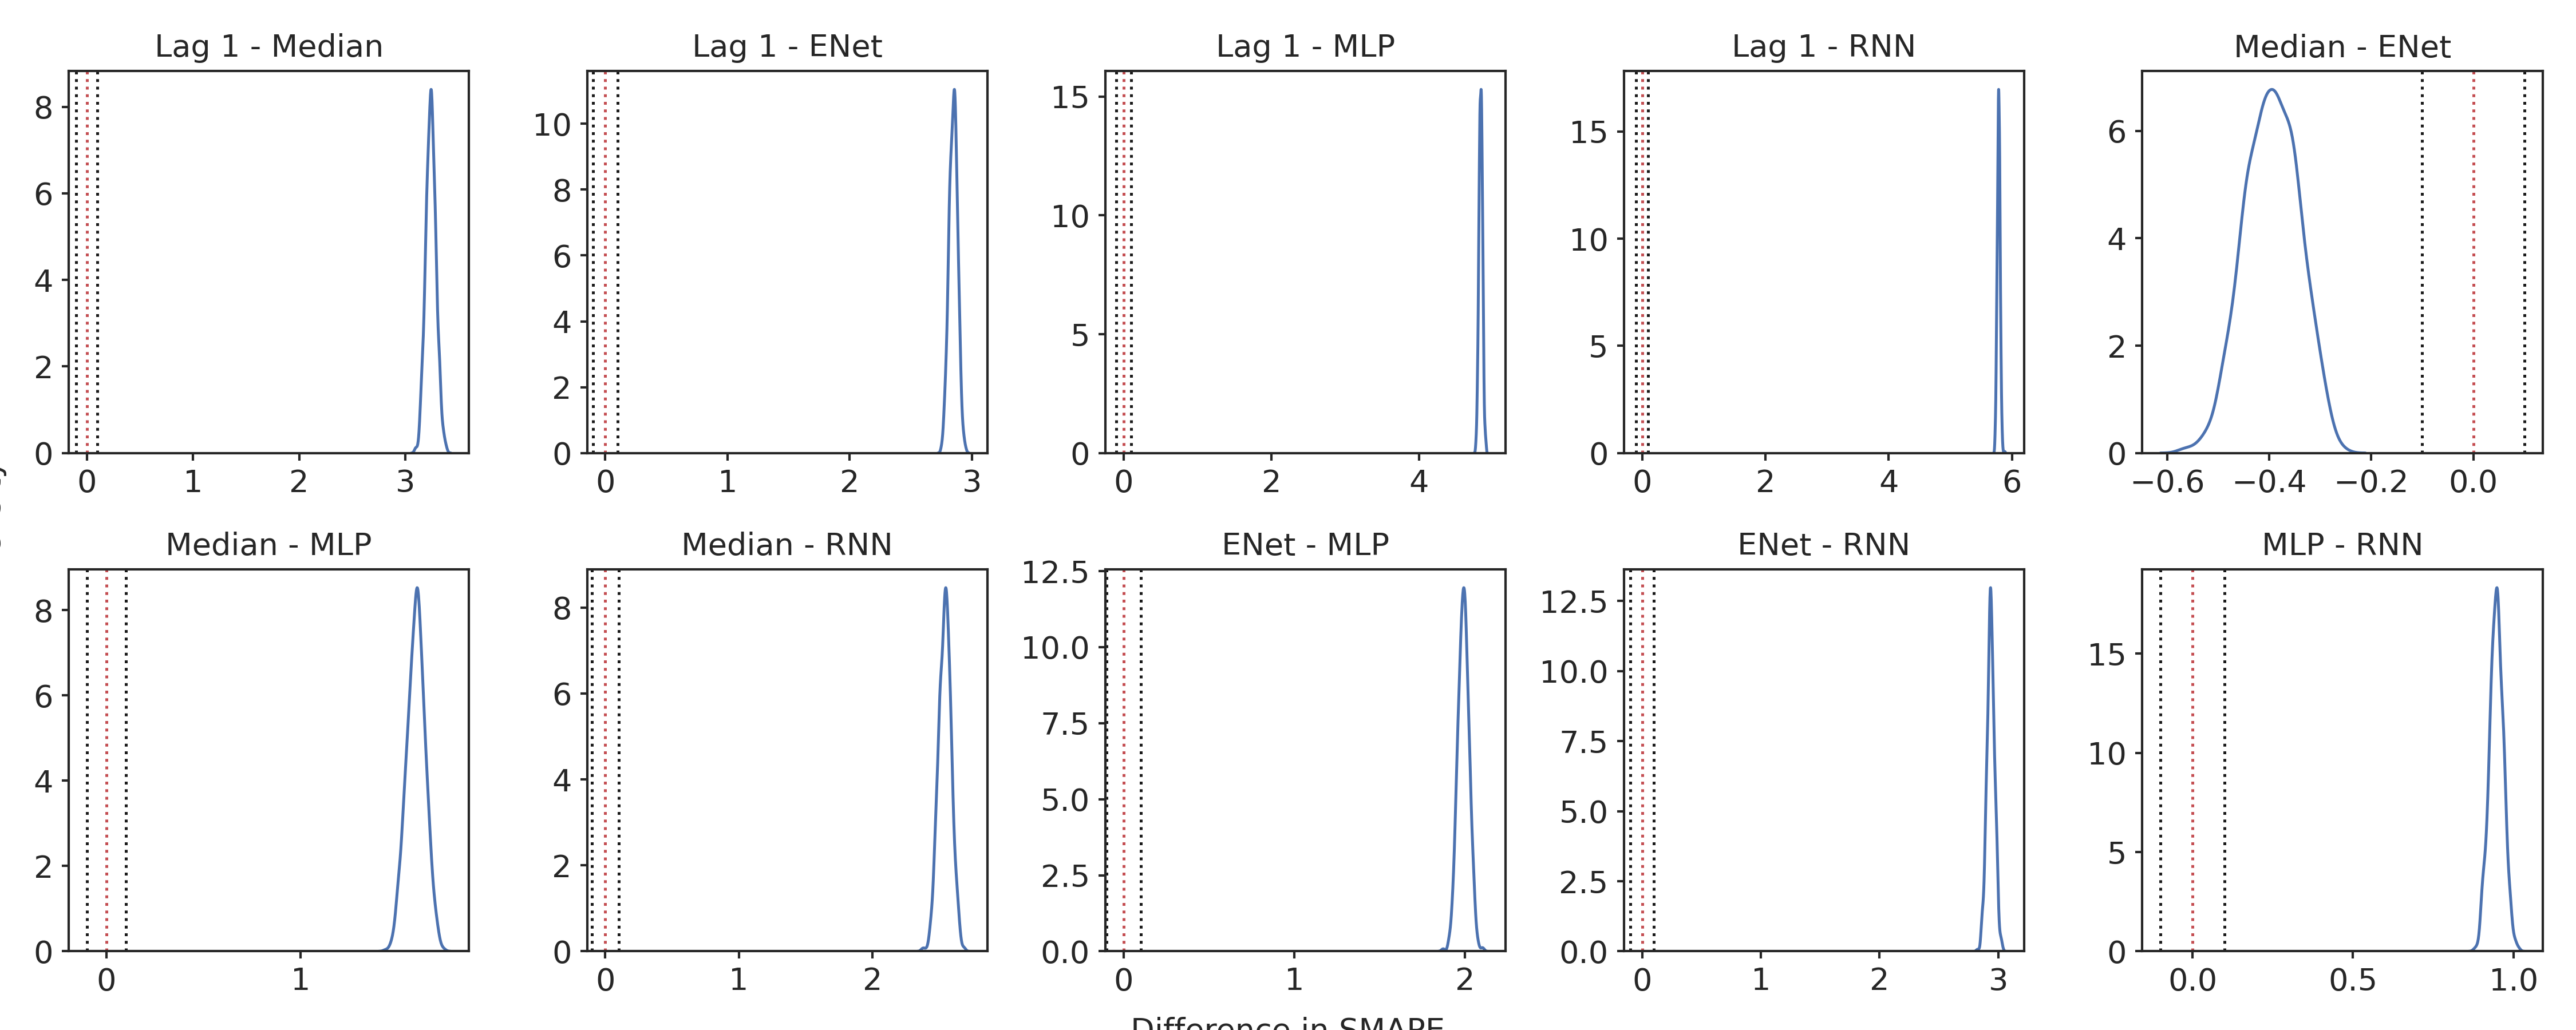
\includegraphics[width=\textwidth]{images/appendix_C/Future_Session_Time_comp_2.png}
\caption[\textbf{Future session time pairwise comparisons of model fixed effect}]{Pairwise comparisons of the parameter $\alpha$ (i.e. model slope) estimated by the model fitted for the Future Session Time target.}
\label{comp_sess_2}
\end{figure}
\FloatBarrier

\subsection{Future Session Activity}
\label{future_acti_bayes_2}

\begin{figure}[ht]
\centering
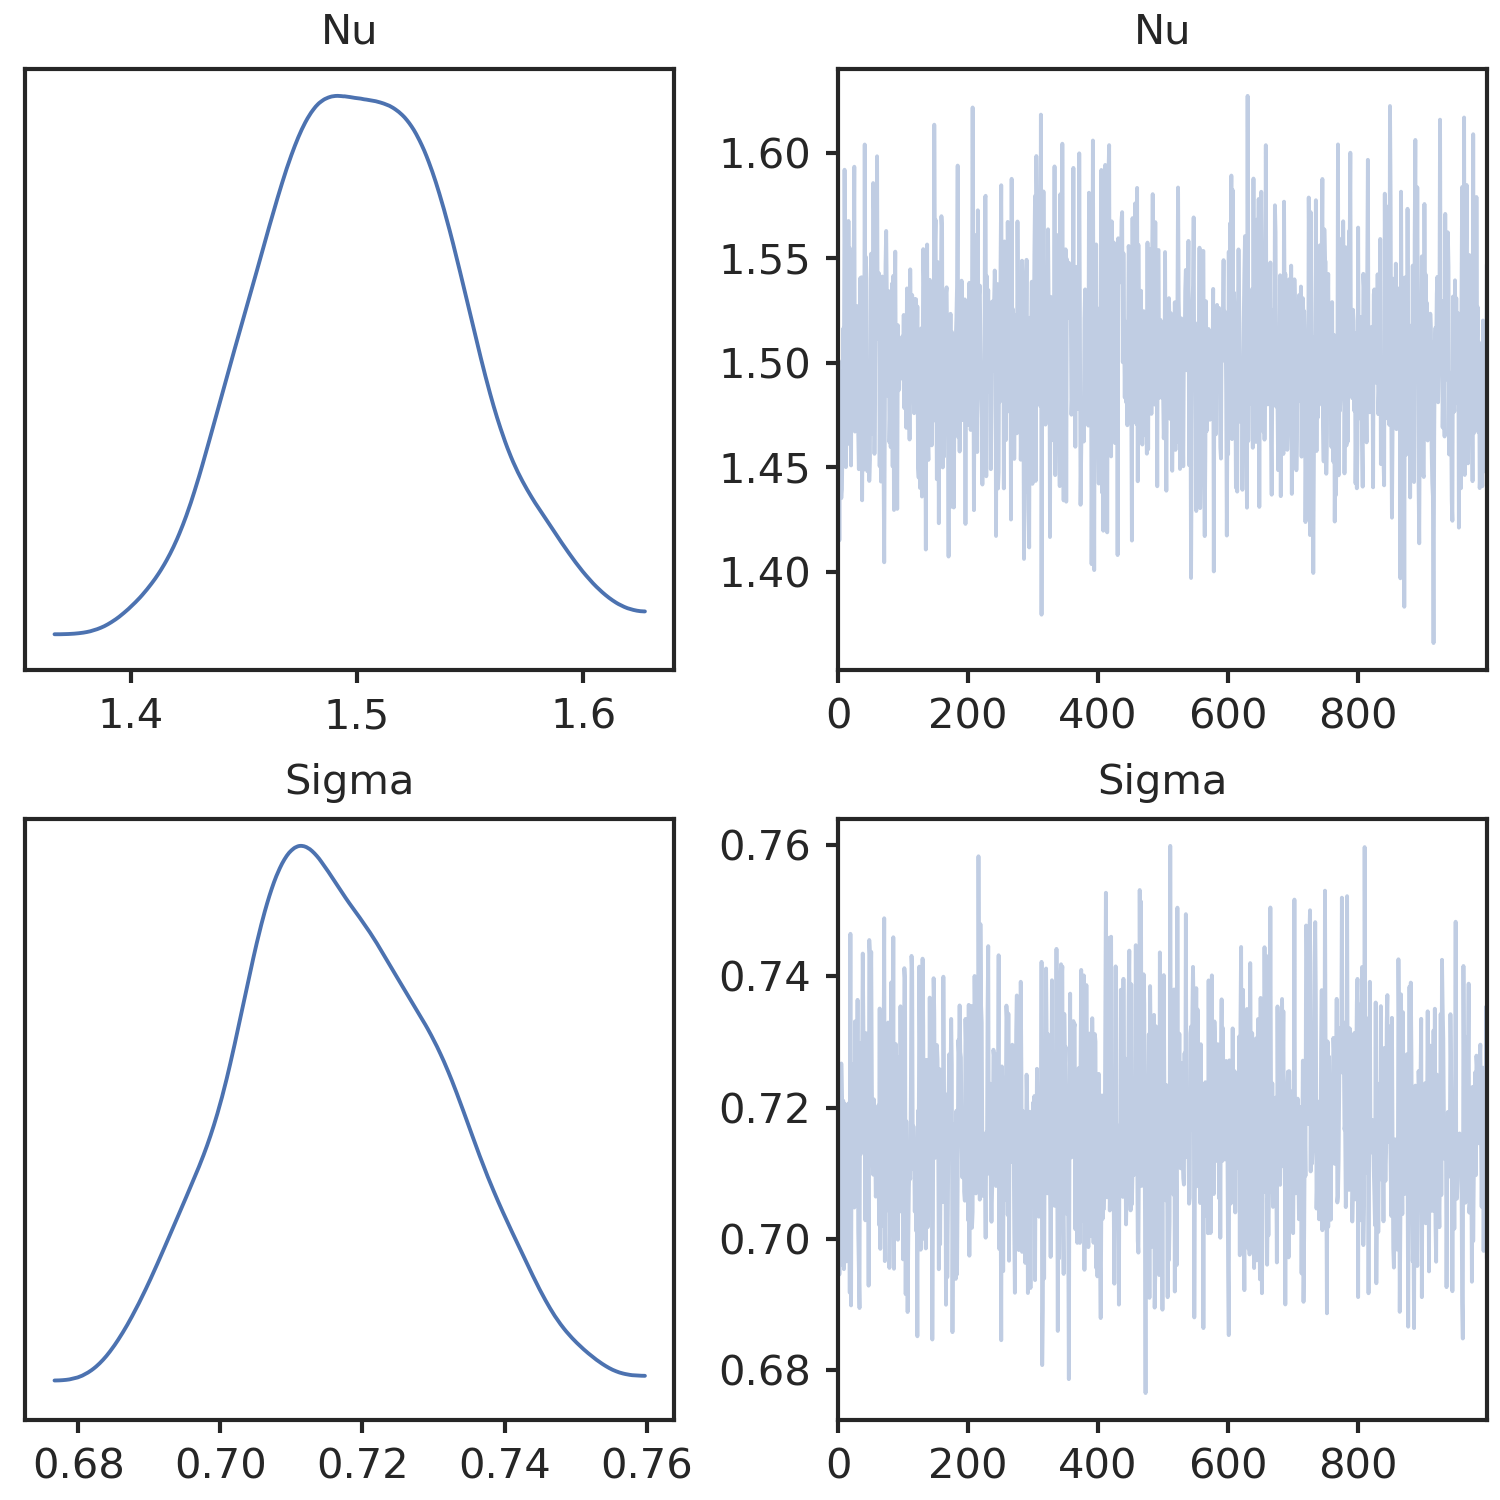
\includegraphics[width=0.5\textwidth]{images/appendix_C/Future Session Activity_marginals_2.png}
\caption[\textbf{Future session activity marginal distributions}]{Marginal distributions for the parameters $\nu$, $\sigma$ estimated by the model fitted for the Future Session Activity target.}
\label{marginals_acti_2}
\end{figure}
\FloatBarrier

\begin{figure}[ht]
\centering
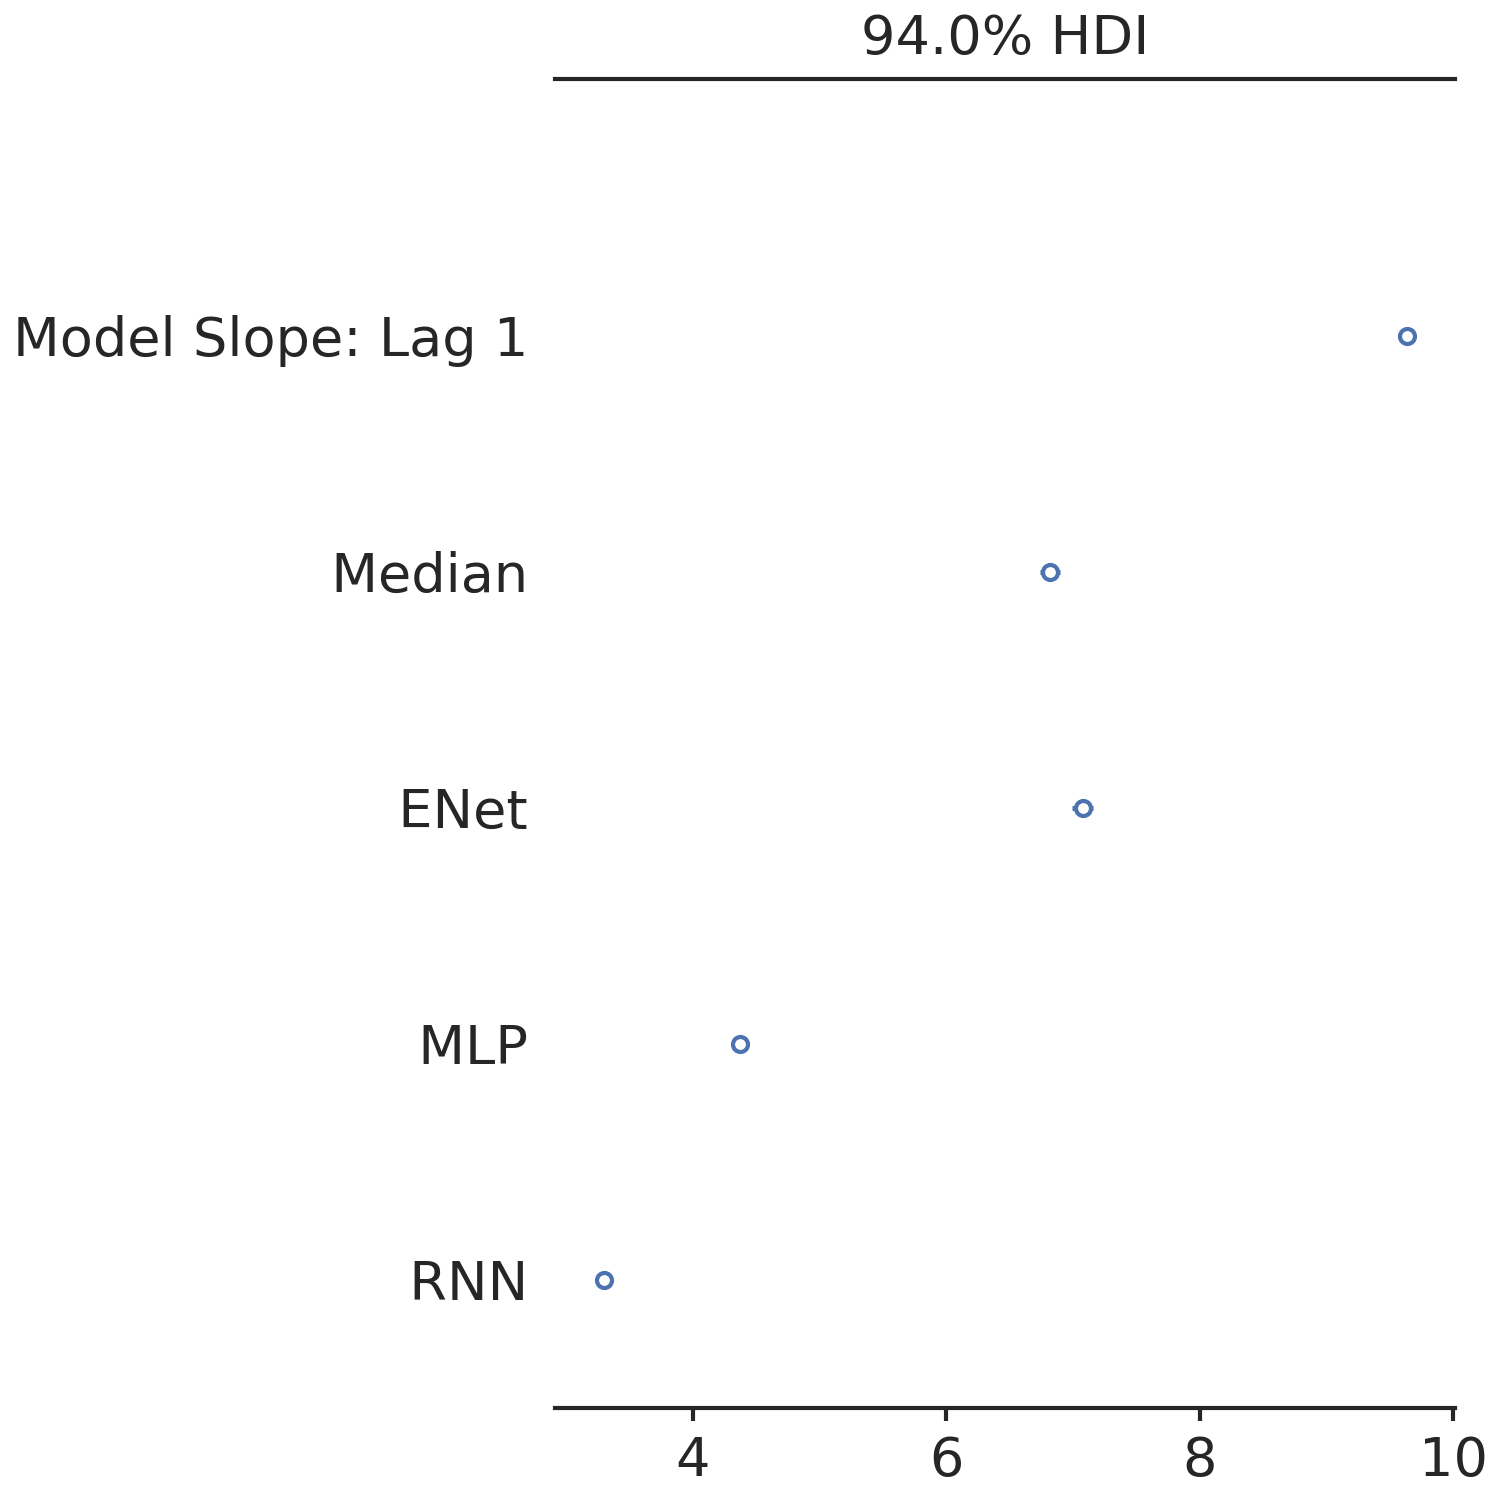
\includegraphics[width=0.5\textwidth]{images/appendix_C/Future Session Activity_models_2.png}
\caption[\textbf{Future session activity model fixed effect}]{Forest plot of the marginal distributions for the parameter $\alpha$ (i.e. model slope) estimated by the model fitted for the Future Session Activity target.}
\label{model_acti_2}
\end{figure}
\FloatBarrier

\begin{figure}[ht]
\centering
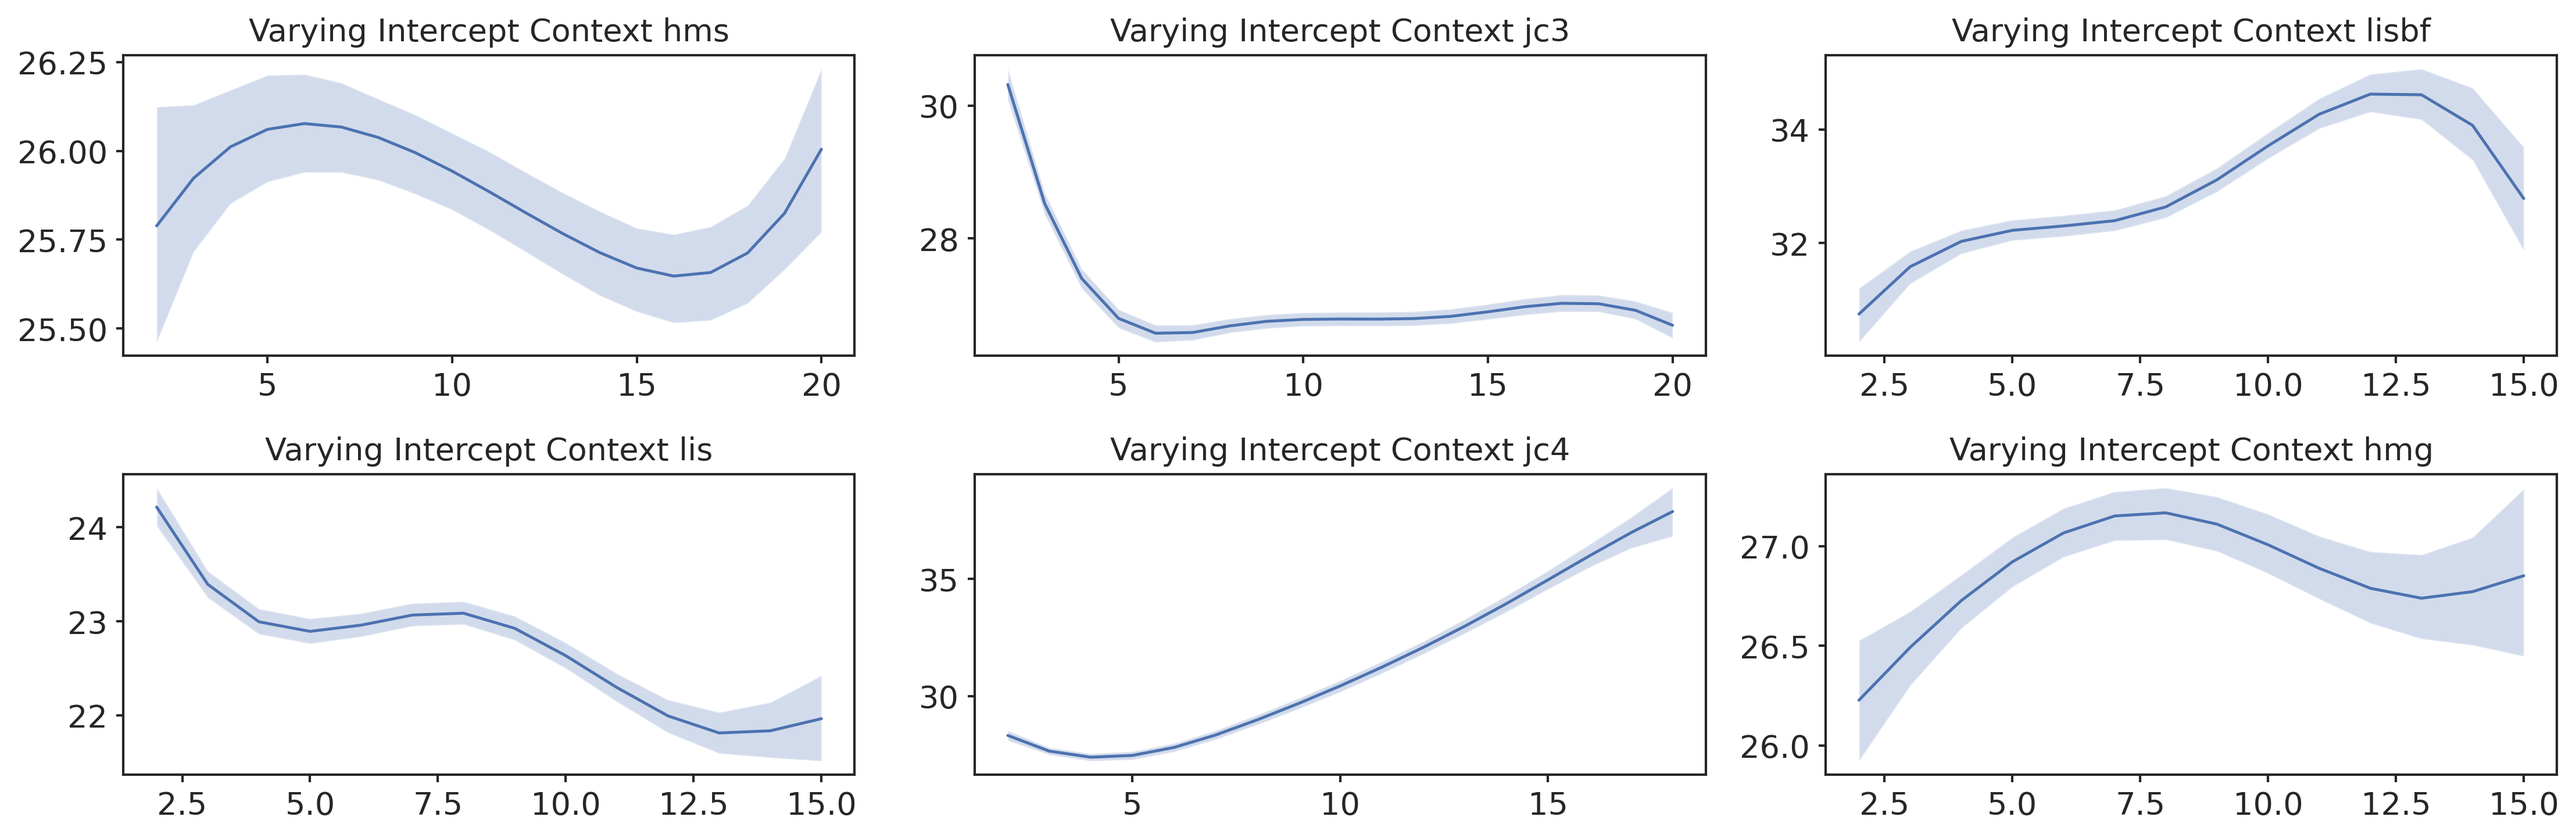
\includegraphics[width=\textwidth]{images/appendix_C/dafaq.png}
\caption[\textbf{Future session activity time-varying random intercept}]{Time varying random intercept estimated by the model fitted for the Future Session Activity target.}
\label{interc_acti_2}
\end{figure}
\FloatBarrier

\begin{figure}[ht]
\centering
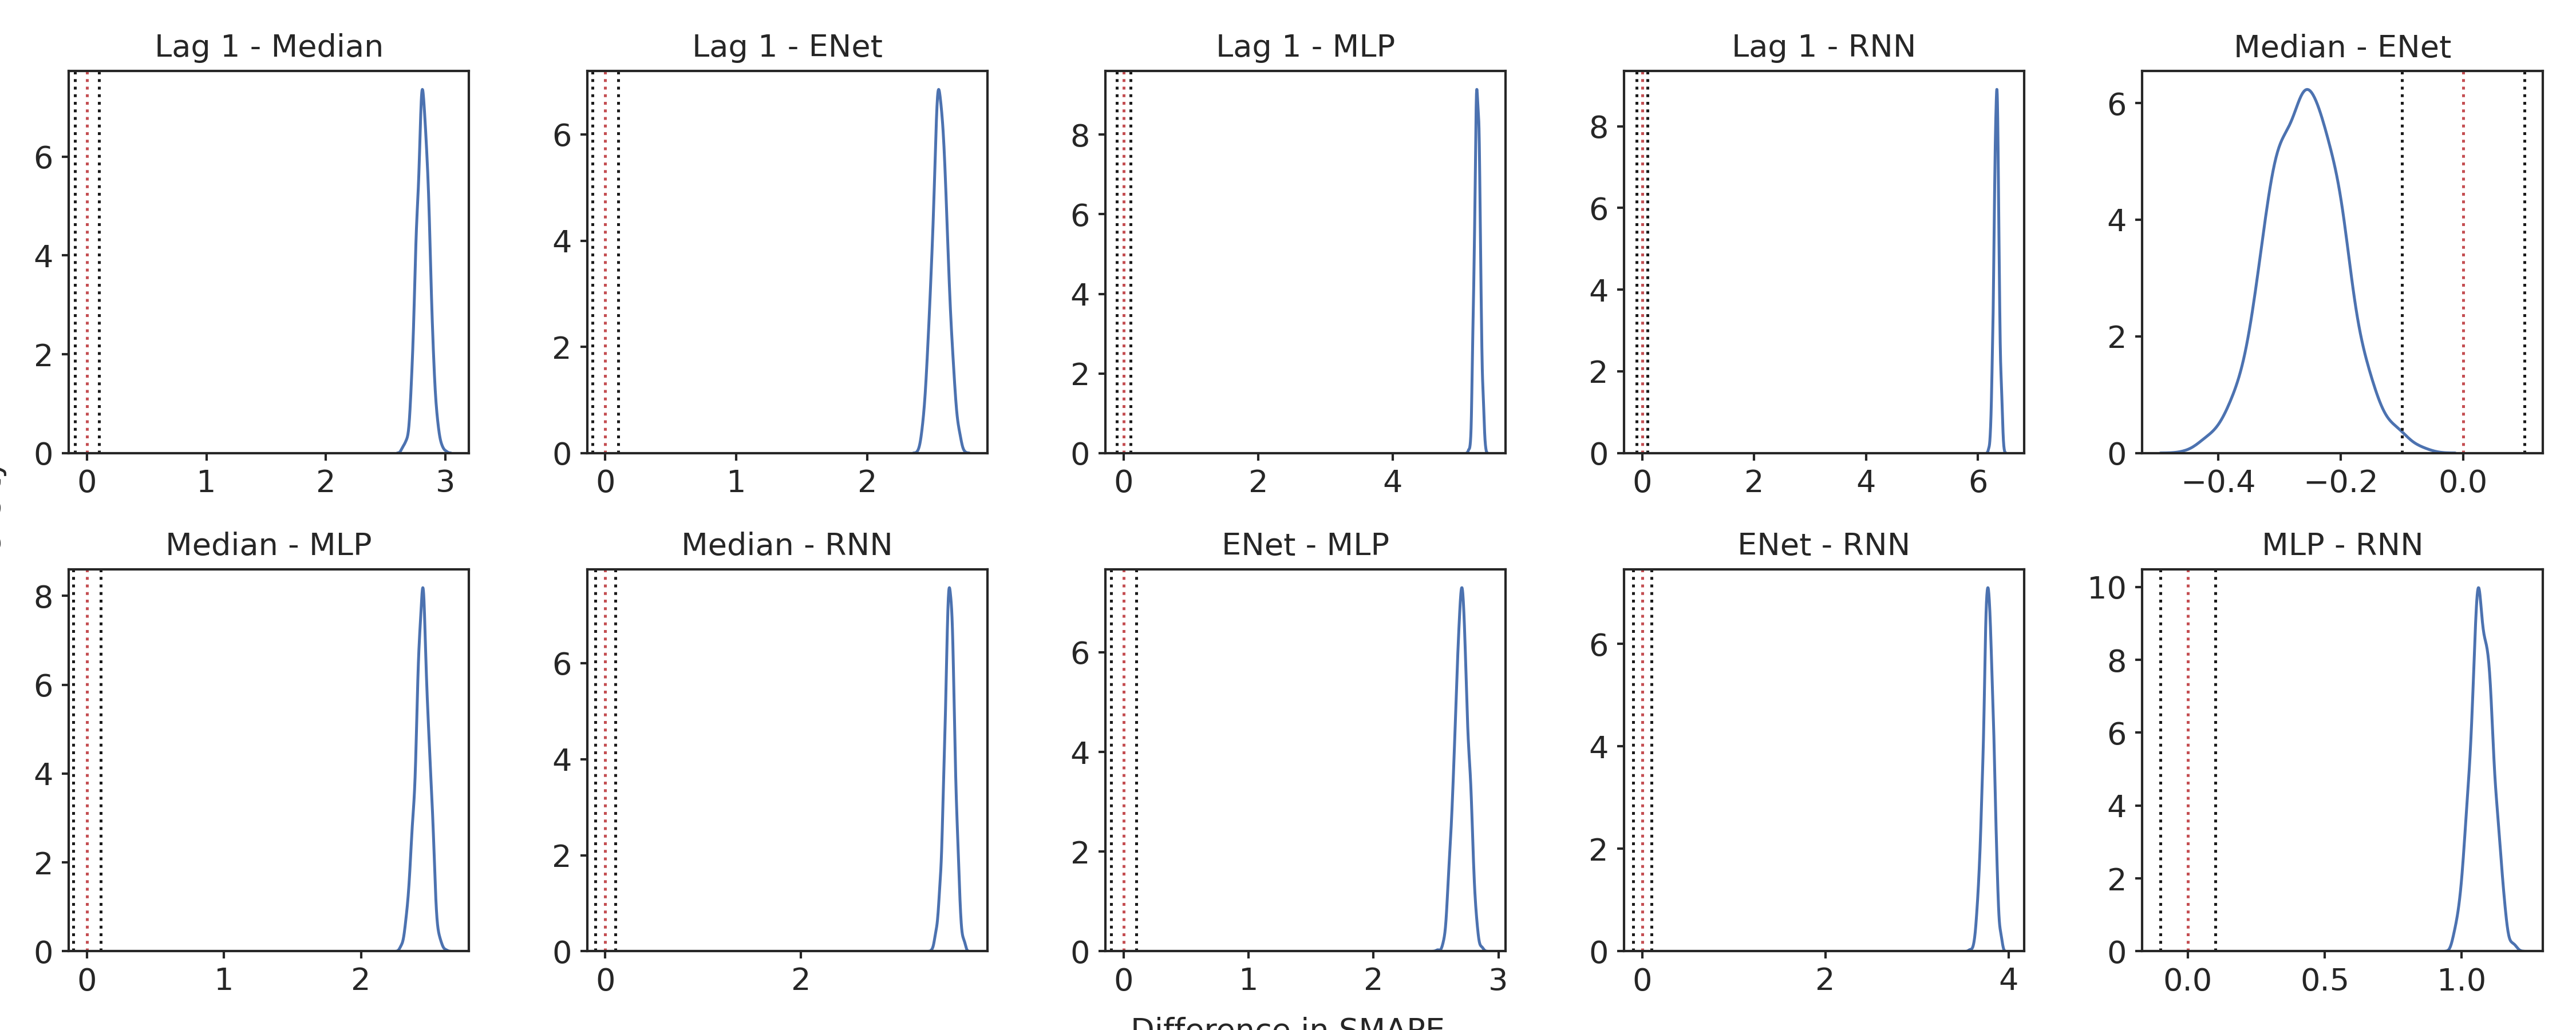
\includegraphics[width=\textwidth]{images/appendix_C/Future_Session_Activity_comp_2.png}
\caption[\textbf{Future session activity pairwise comparisons of model fixed effect}]{Pairwise comparisons of the parameter $\alpha$ (i.e. model slope) estimated by the model fitted for the Future Session Activity target.}
\label{comp_acti_2}
\end{figure}
\FloatBarrier

\subsection{Future N° Sessions}
\label{future_no_sess_bayes_2}

\begin{figure}[ht]
\centering
\includegraphics[width=0.5\textwidth]{images/appendix_C/Future N° Sessions_marginals_2.png}
\caption[\textbf{Future N°sessions marginal distributions}]{Marginal distributions for the parameters $\nu$, $\sigma$ estimated by the model fitted for the Future N°sessions target.}
\label{marginals_no_sess_2}
\end{figure}
\FloatBarrier

\begin{figure}[ht]
\centering
\includegraphics[width=0.5\textwidth]{images/appendix_C/Future N° Sessions_models_2.png}
\caption[\textbf{Future N°sessions model fixed effect}]{Forest plot of the marginal distributions for the parameter $\alpha$ (i.e. model slope) estimated by the model fitted for the Future N°sessions target.}
\label{model_no_sess_2}
\end{figure}
\FloatBarrier

\begin{figure}[ht]
\centering
\includegraphics[width=\textwidth]{images/appendix_C/Future N° Sessions_interc_2.png}
\caption[\textbf{Future N°sessions time-varying random intercept}]{Time varying random intercept estimated by the model fitted for the Future N°sessions target.}
\label{interc_no_sess_2}
\end{figure}
\FloatBarrier

\begin{figure}[ht]
\centering
\includegraphics[width=\textwidth]{images/appendix_C/Future_N°_Sessions_comp_2.png}
\caption[\textbf{Future N°sessions pairwise comparisons of model fixed effect}]{Pairwise comparisons of the parameter $\alpha$ (i.e. model slope) estimated by the model fitted for the Future N°sessions target.}
\label{comp_no_sess_2}
\end{figure} \FloatBarrier

\section{Dynamic Prediction of Future Behavioural Intensity with Environmental and Game Covariates}
\label{dynamic_env_even_prediction_ancillary_perf}

We report here the results of fitting the Bayesian model to the perfromance data obtained from the experimental task described in section \ref{model_architecture_3}.

\subsection{Targets Collapsed}
\label{collapsed_bayes_3}

\begin{figure}[ht]
\centering
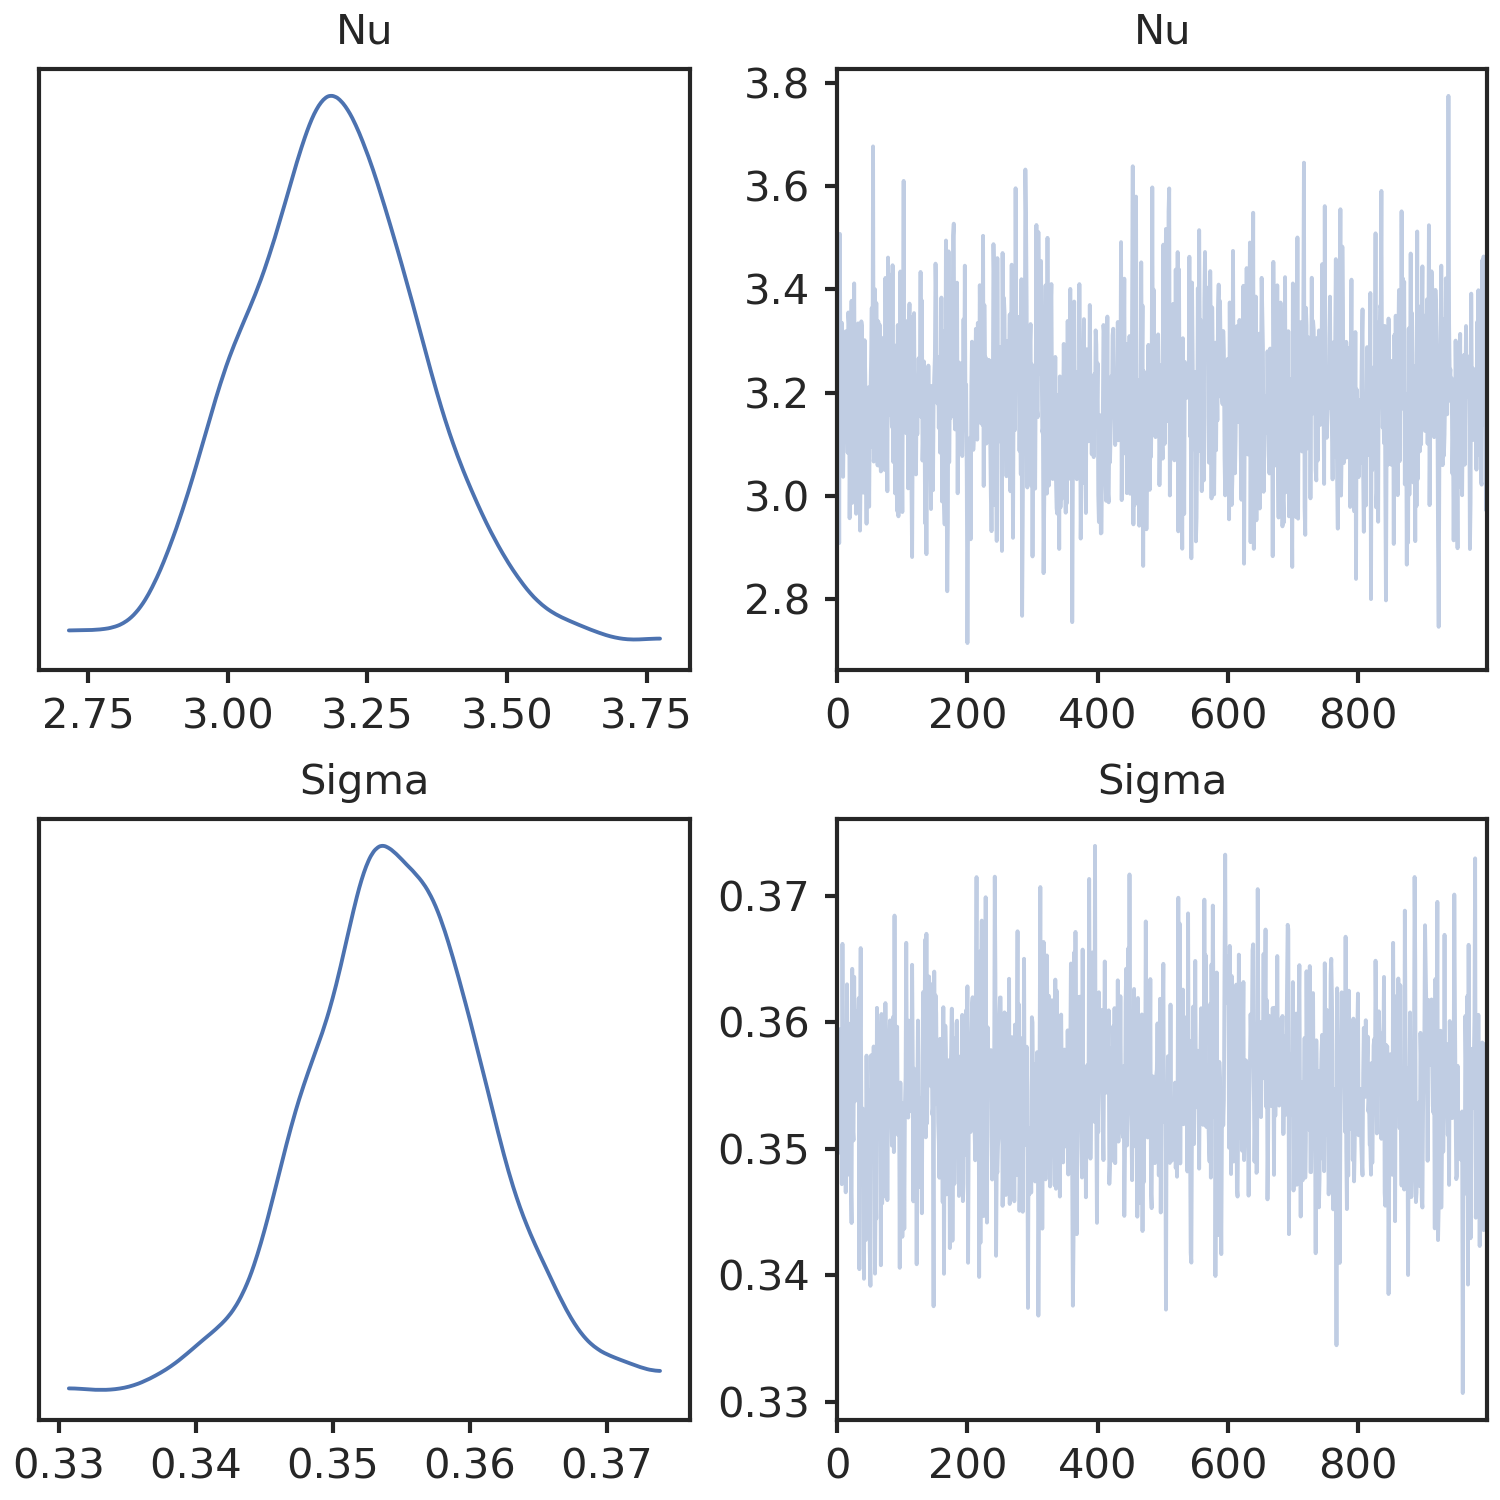
\includegraphics[width=0.5\textwidth]{images/appendix_C/collapsed_marginals_3.png}
\caption[\textbf{Targets collapsed marginal distributions}]{Marginal distributions for the parameters $\nu$, $\sigma$ estimated by the model fitted for the Future Absence target.}
\label{marginals_coll_3}
\end{figure} \FloatBarrier

\begin{figure}[ht]
\centering
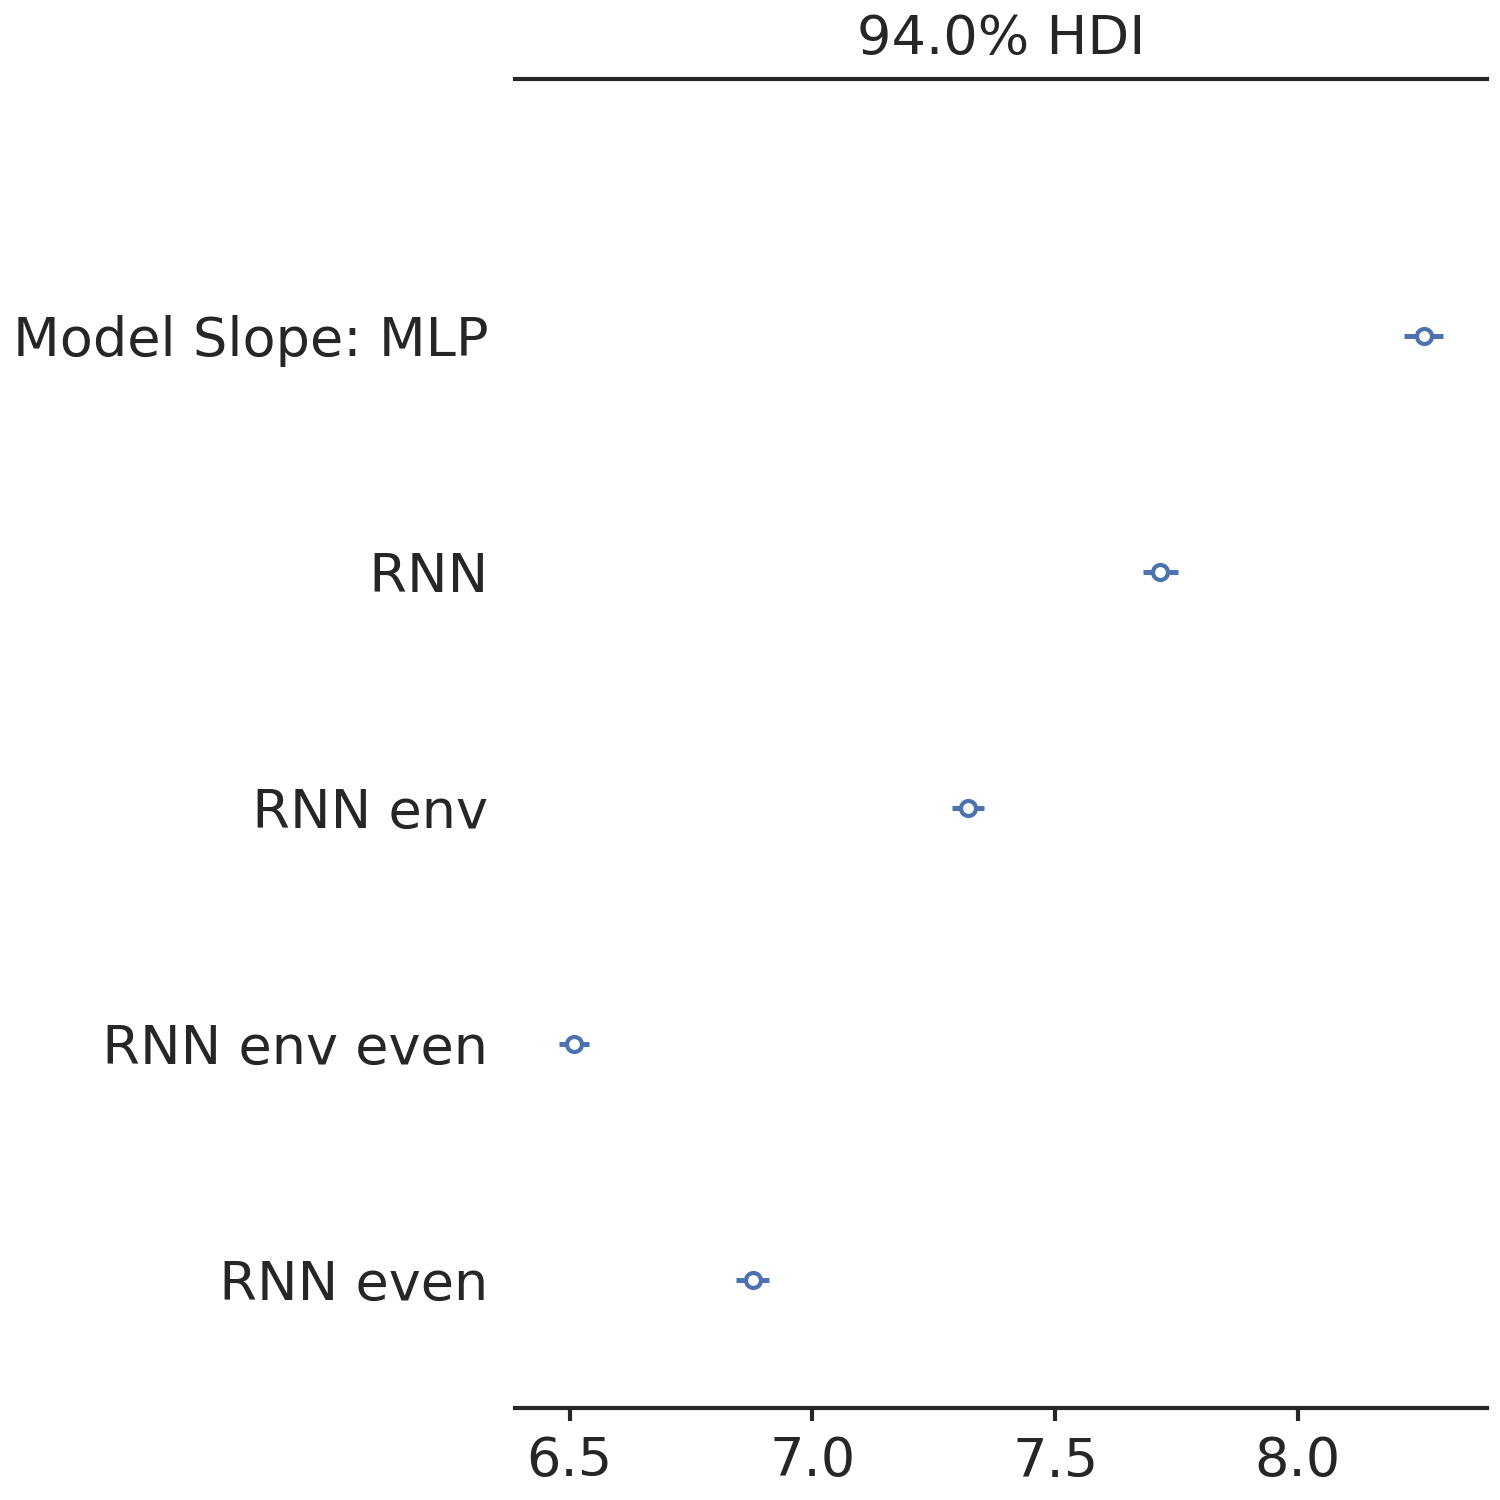
\includegraphics[width=0.5\textwidth]{images/appendix_C/collapsed_models_3.png}
\caption[\textbf{Targets collapsed model fixed effect}]{Forest plot of the marginal distributions for the parameter $\alpha$ (i.e. model slope) estimated by the model fitted for the Future Absence target.}
\label{model_coll_3}
\end{figure} \FloatBarrier

\begin{figure}[ht]
\centering
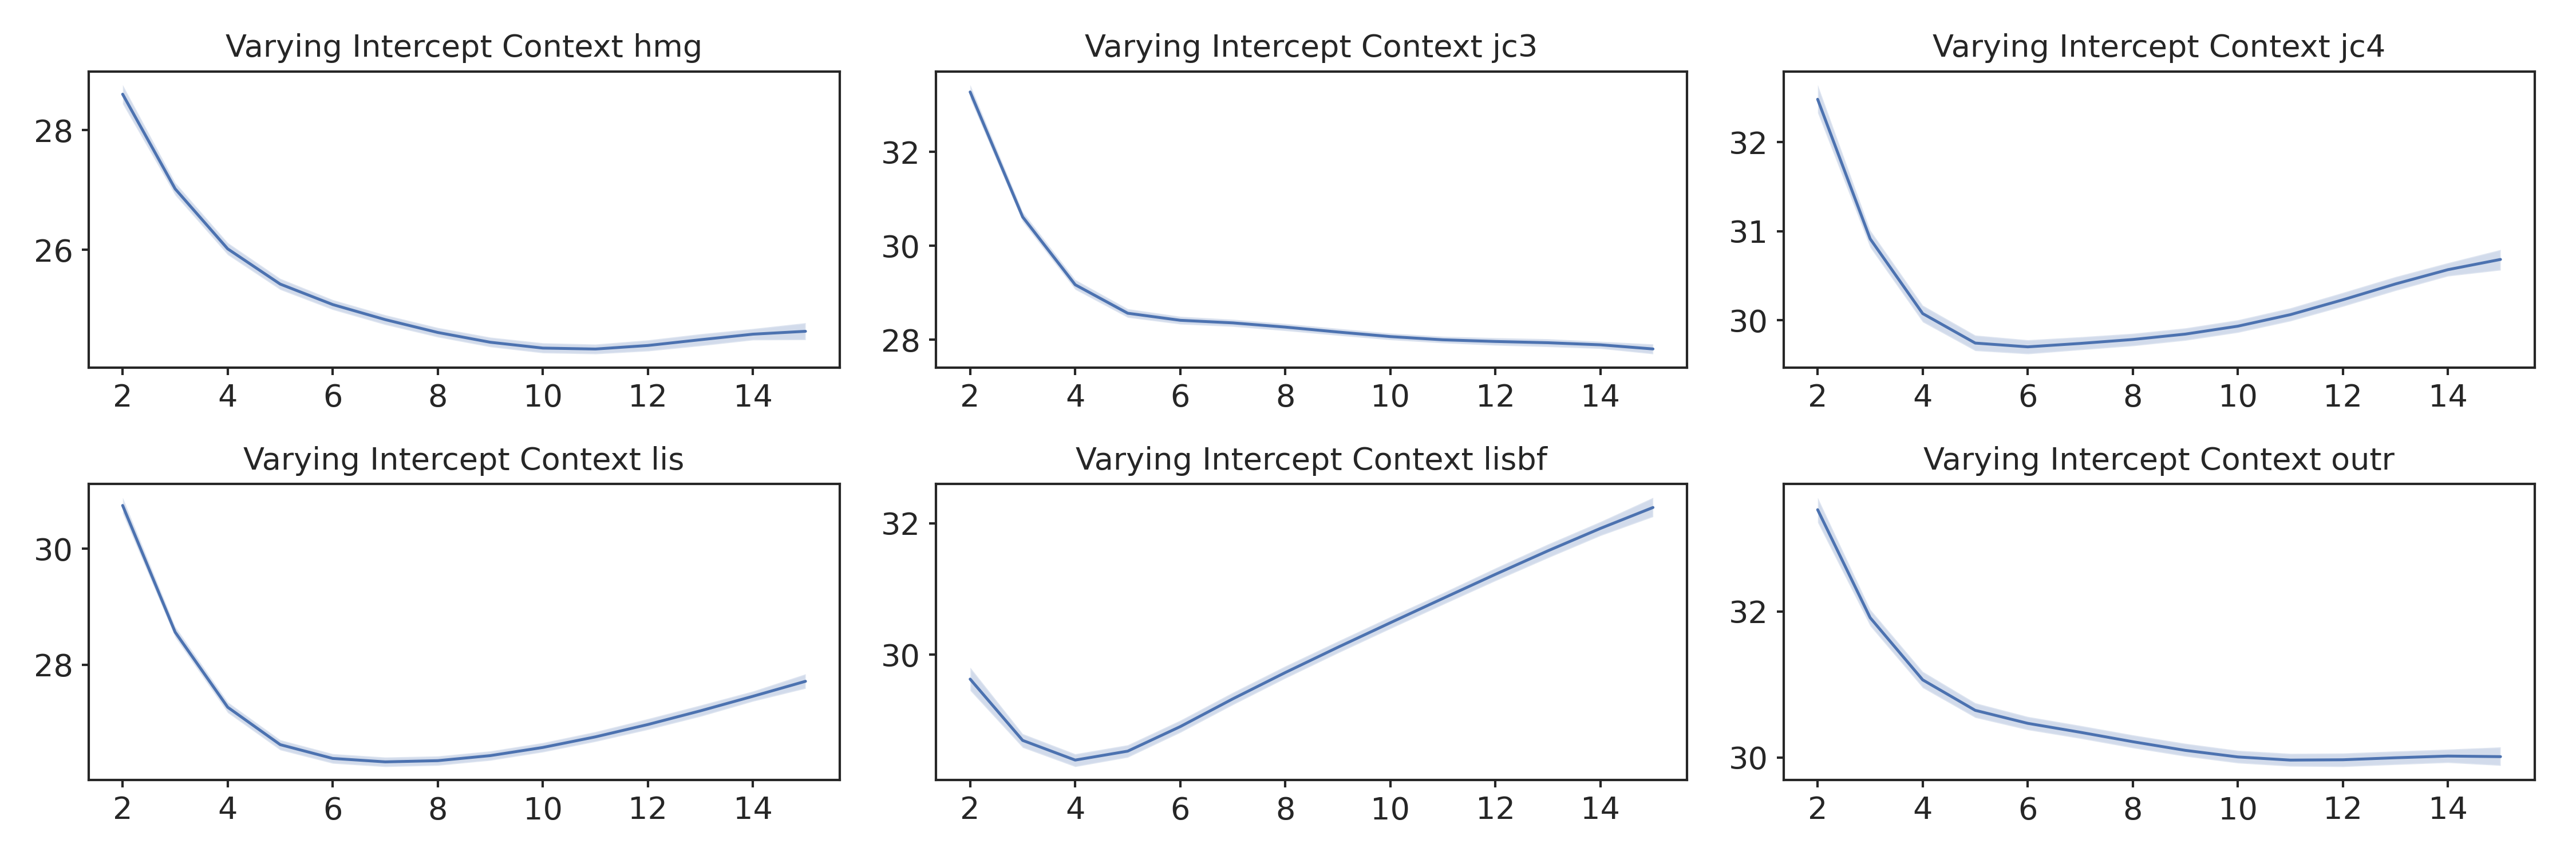
\includegraphics[width=\textwidth]{images/appendix_C/collapsed_interc_3.png}
\caption[\textbf{Targets collapsed time-varying random intercept}]{Time varying random intercept estimated by the model fitted for the Future Absence target.}
\label{interc_coll_3}
\end{figure} \FloatBarrier

\begin{figure}[ht]
\centering
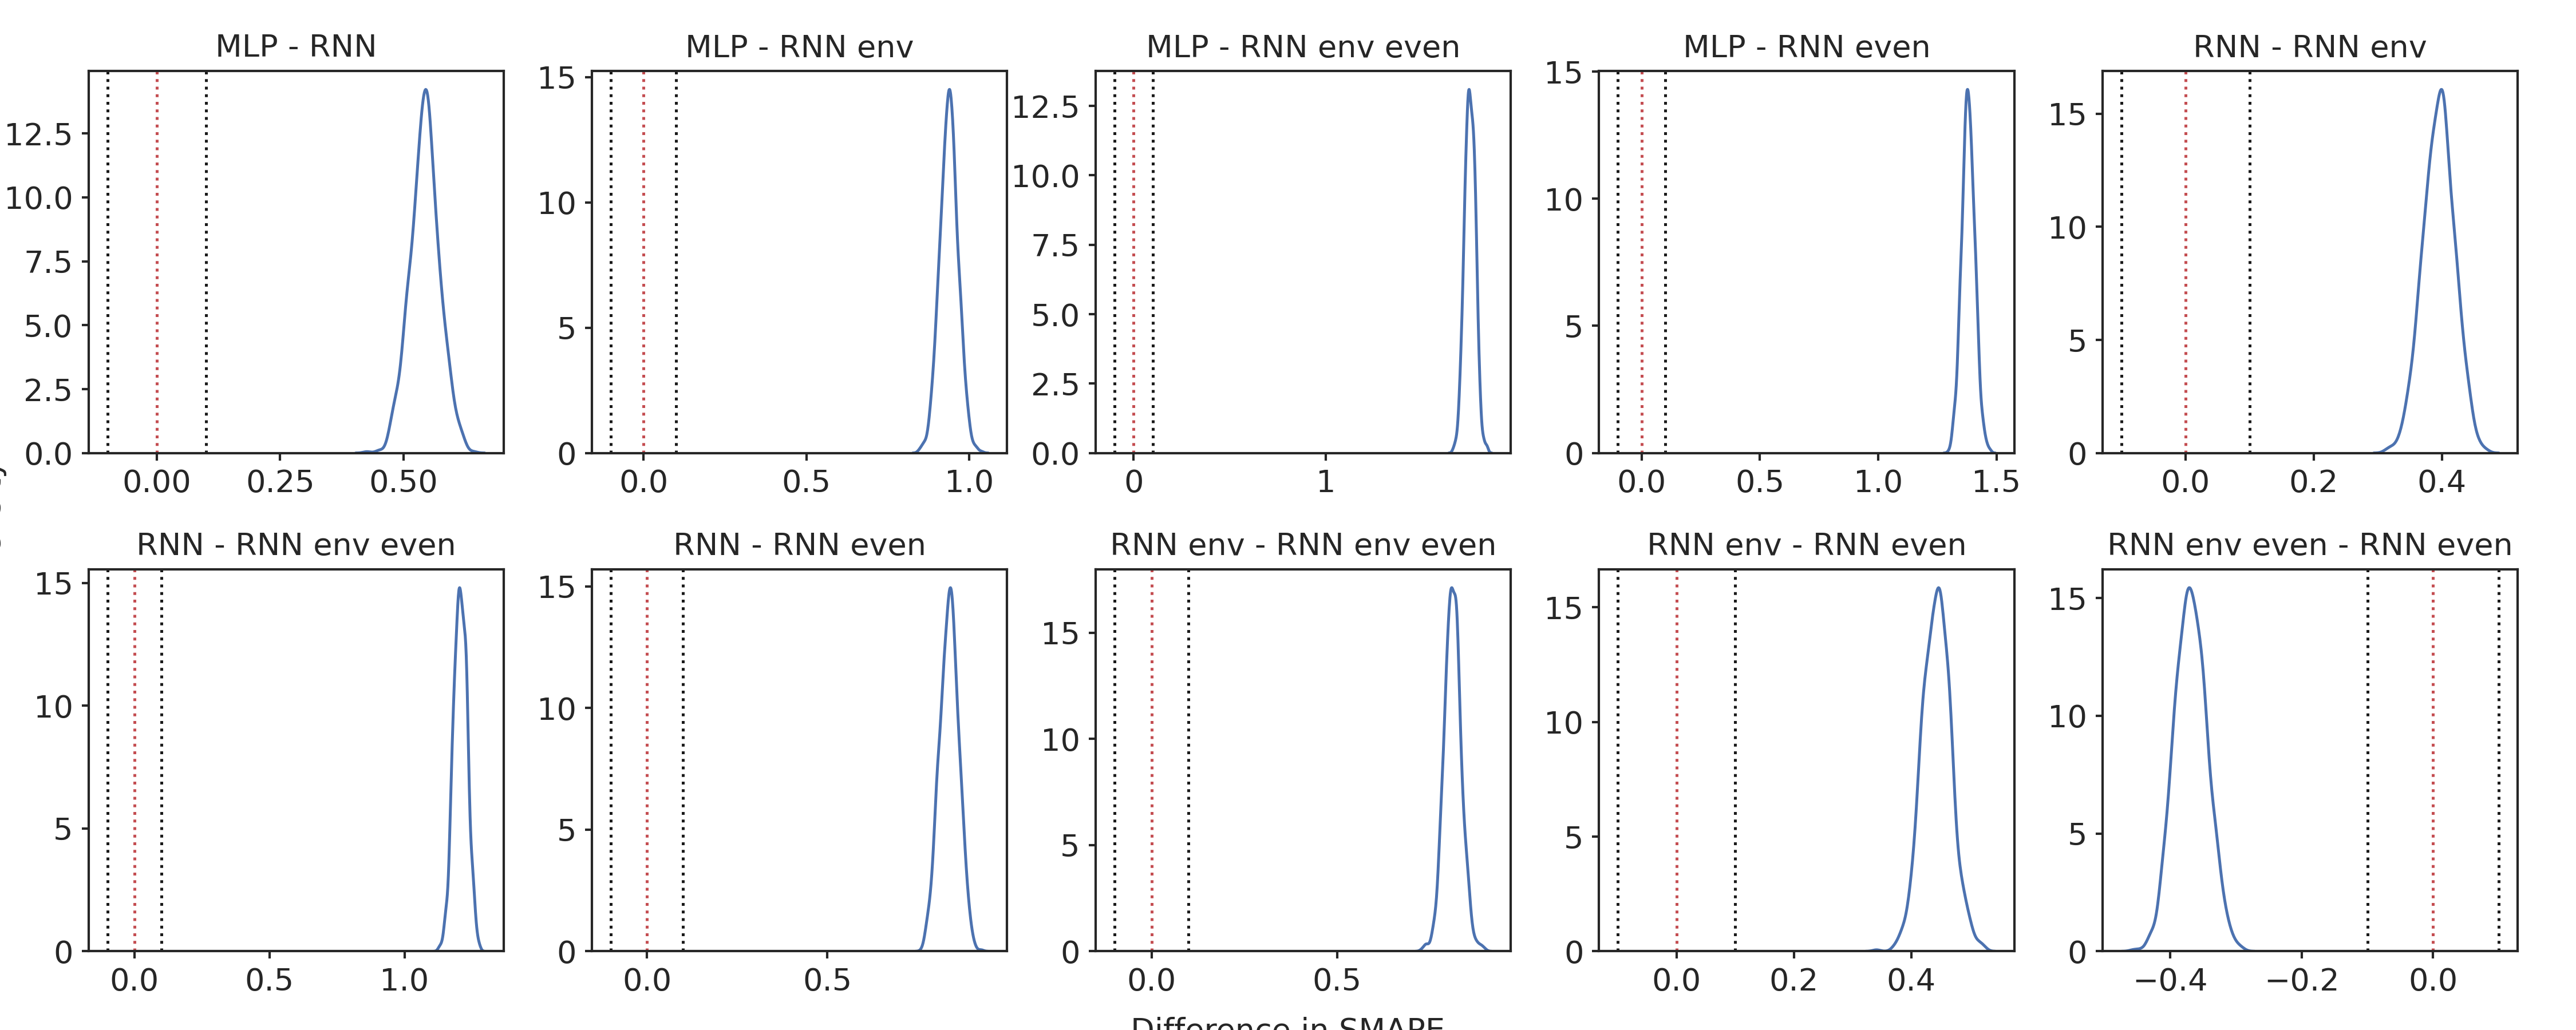
\includegraphics[width=\textwidth]{images/appendix_C/collapsed_comp_3.png}
\caption[\textbf{Targets collapsed pairwise comparisons of model fixed effect}]{Pairwise comparisons of the parameter $\alpha$ (i.e. model slope) estimated by the model fitted for the Future Absence target.}
\label{comp_coll_3}
\end{figure} \FloatBarrier

\subsection{Future Absence}
\label{future_abs_bayes_3}

\begin{figure}[ht]
\centering
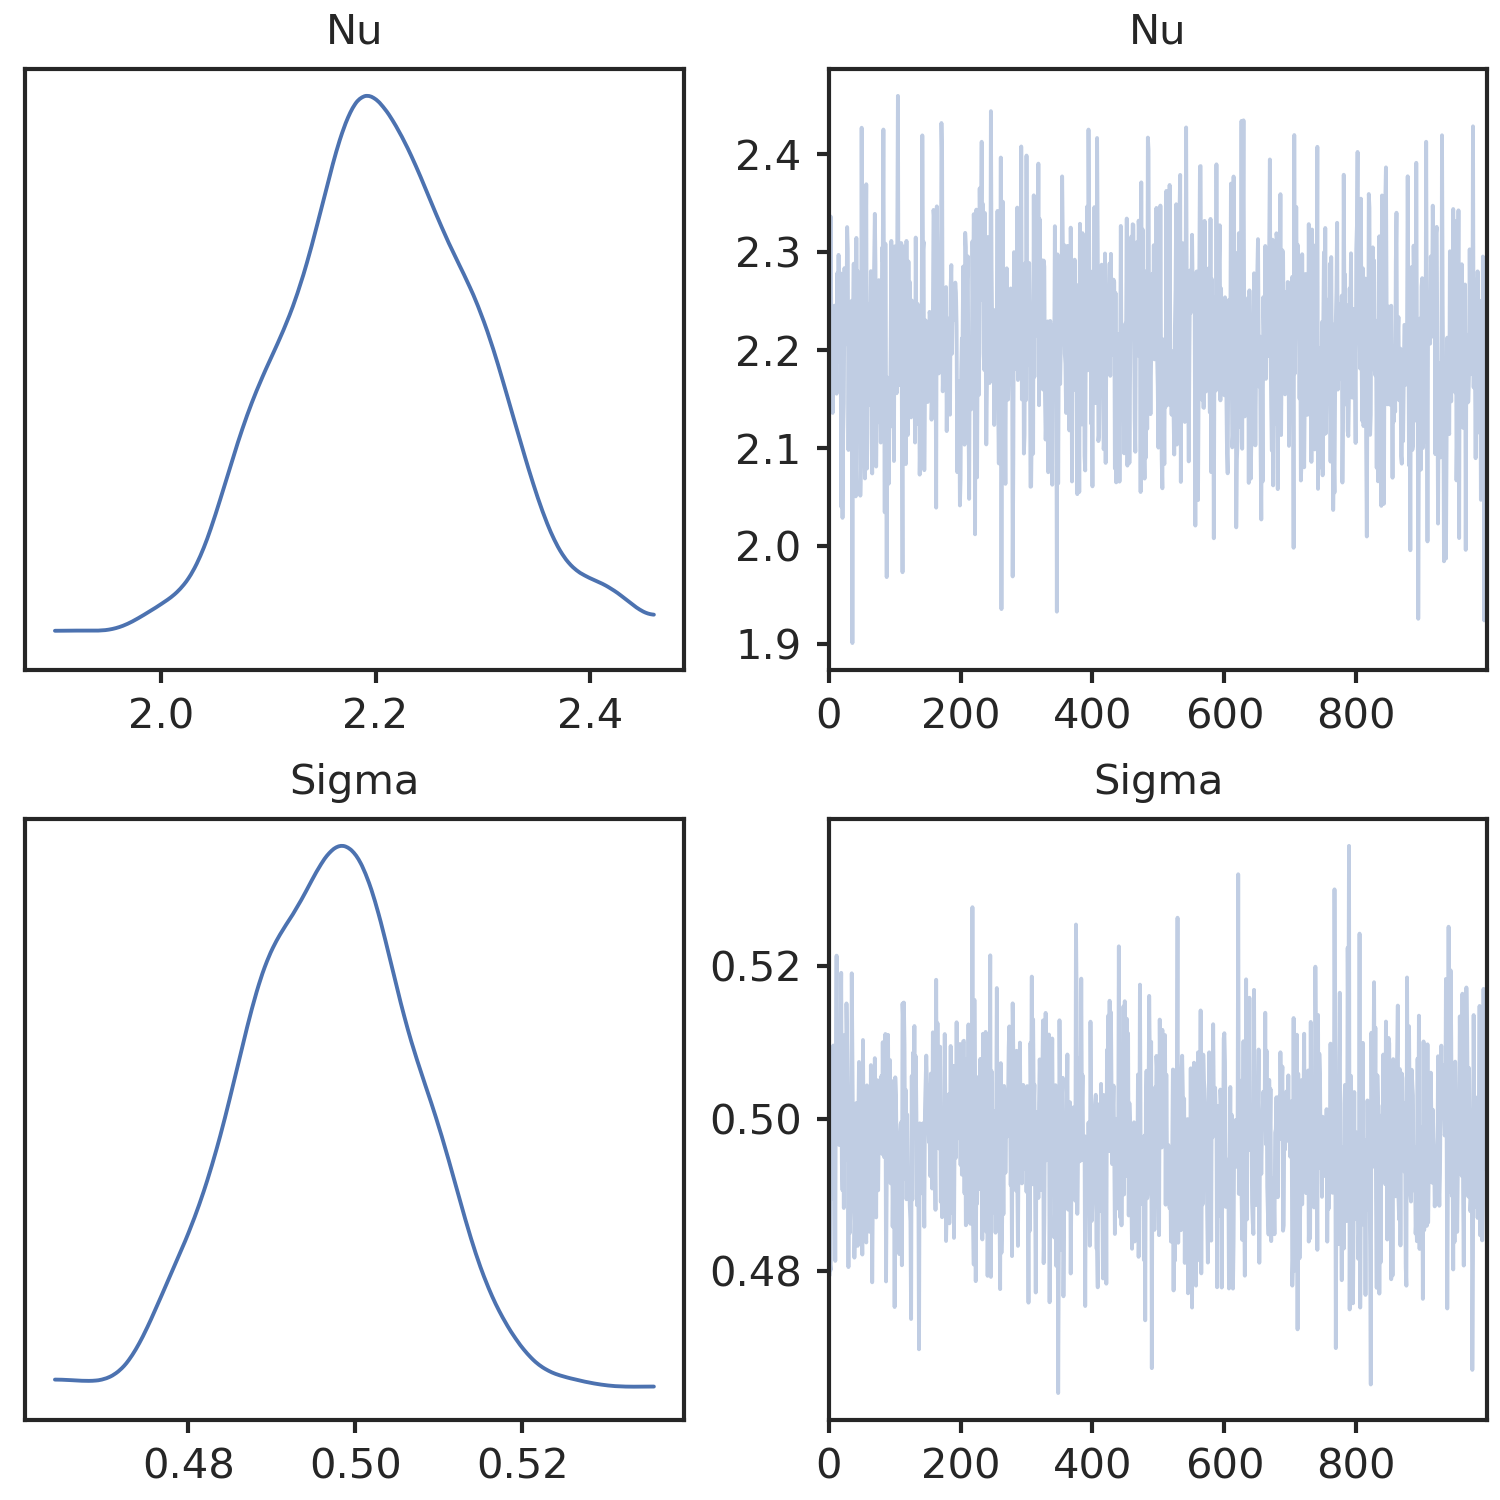
\includegraphics[width=0.5\textwidth]{images/appendix_C/Future Absence_marginals_3.png}
\caption[\textbf{Future absence marginal distributions}]{Marginal distributions for the parameters $\nu$, $\sigma$ estimated by the model fitted for the Future Absence target.}
\label{marginals_abs_3}
\end{figure} \FloatBarrier

\begin{figure}[ht]
\centering
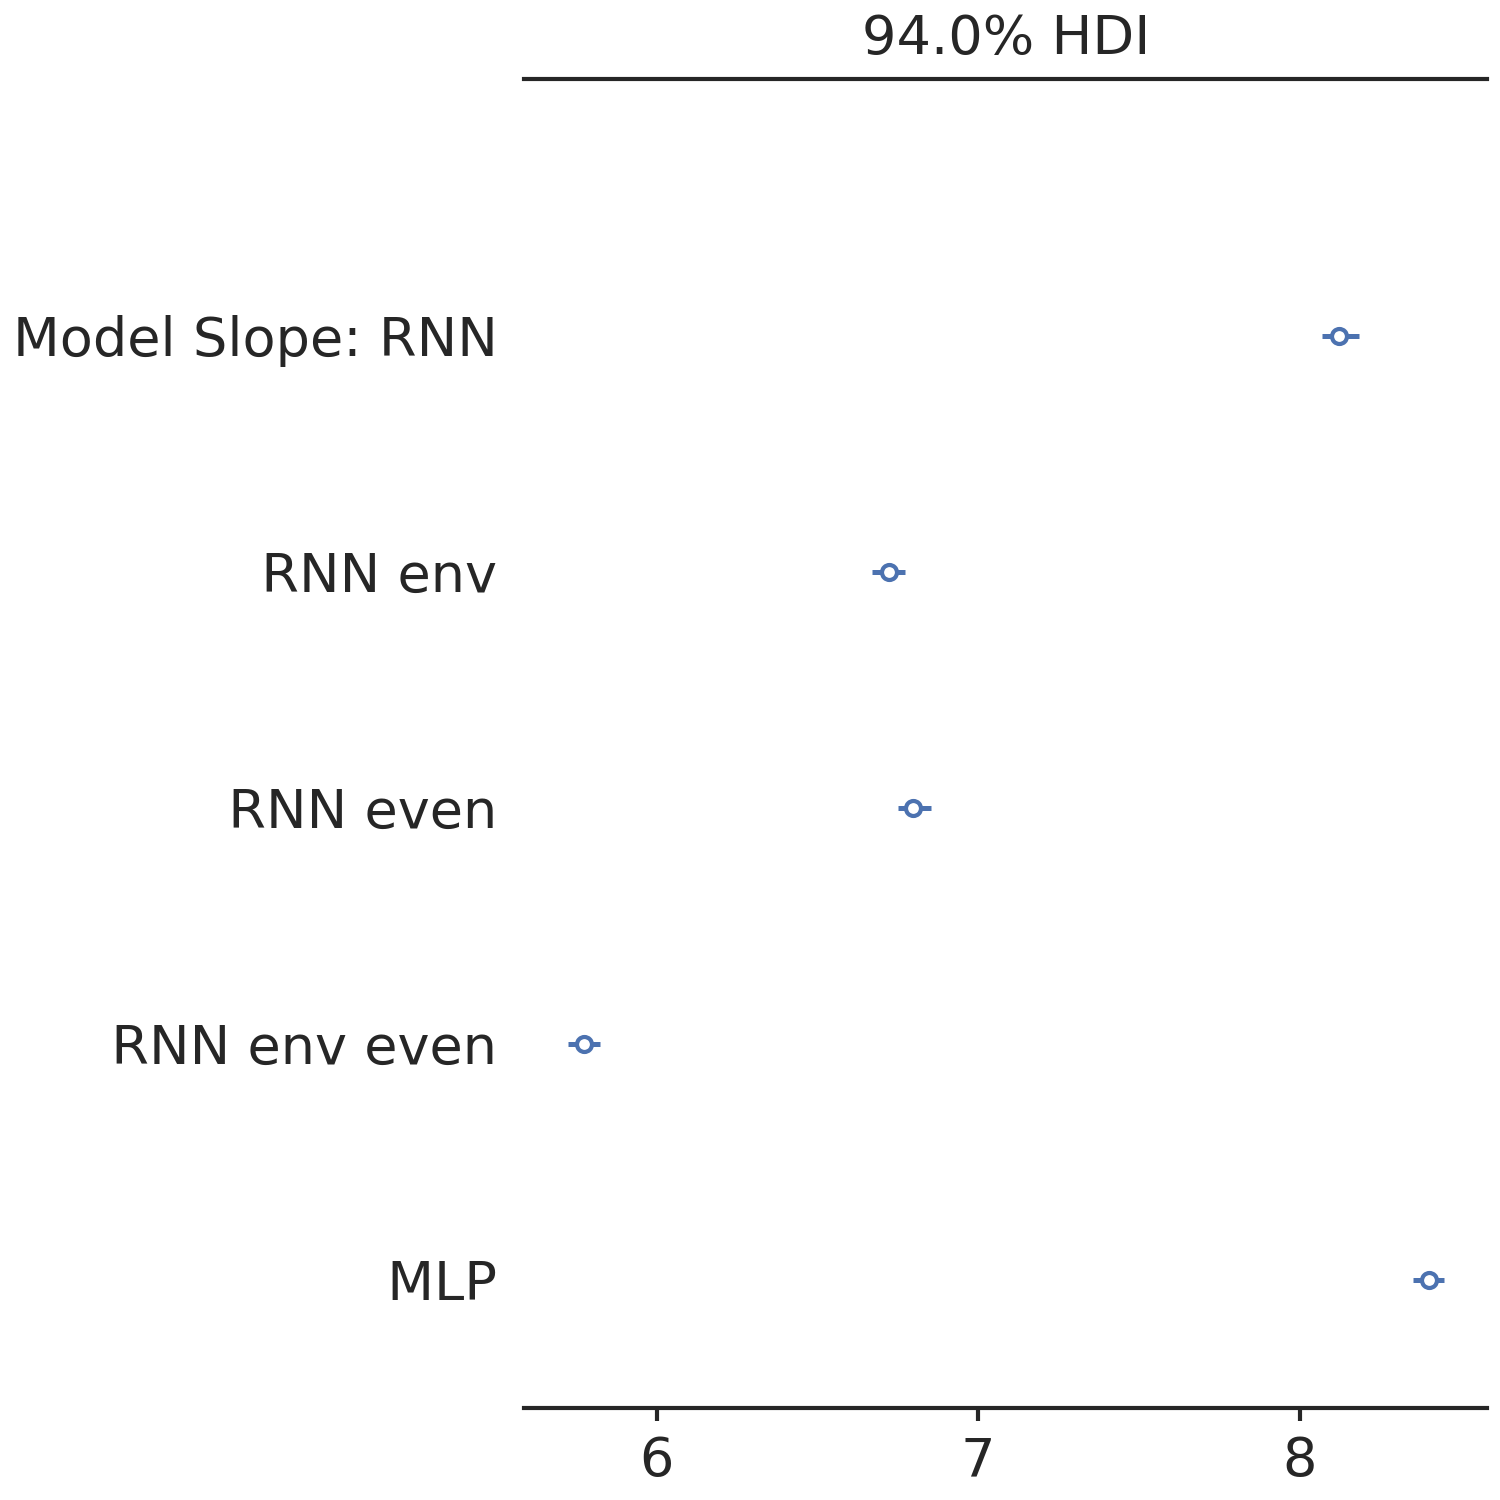
\includegraphics[width=0.5\textwidth]{images/appendix_C/Future Absence_models_3.png}
\caption[\textbf{Future absence model fixed effect}]{Forest plot of the marginal distributions for the parameter $\alpha$ (i.e. model slope) estimated by the model fitted for the Future Absence target.}
\label{model_abs_3}
\end{figure} \FloatBarrier

\begin{figure}[ht]
\centering
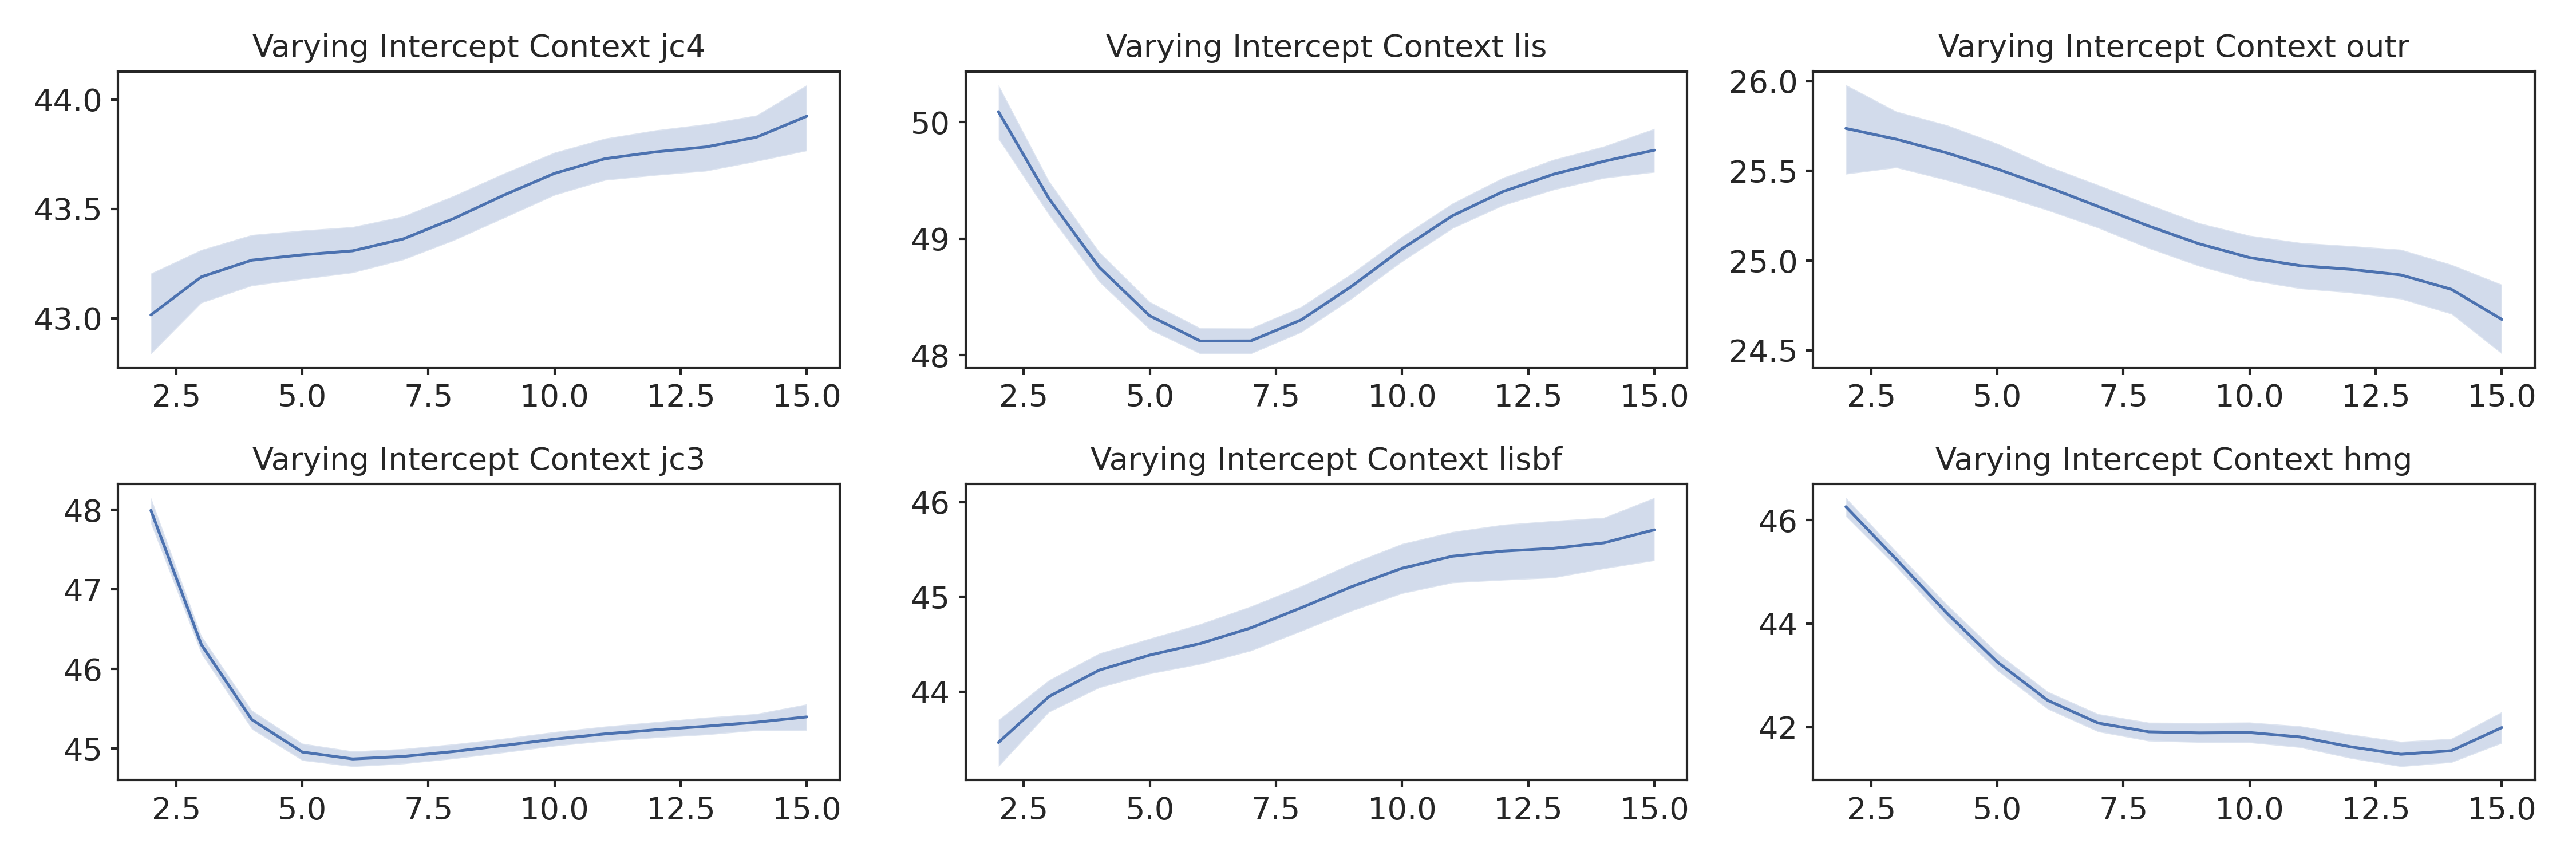
\includegraphics[width=\textwidth]{images/appendix_C/Future Absence_interc_3.png}
\caption[\textbf{Future absence time-varying random intercept}]{Time varying random intercept estimated by the model fitted for the Future Absence target.}
\label{interc_abs_3}
\end{figure} \FloatBarrier

\begin{figure}[ht]
\centering
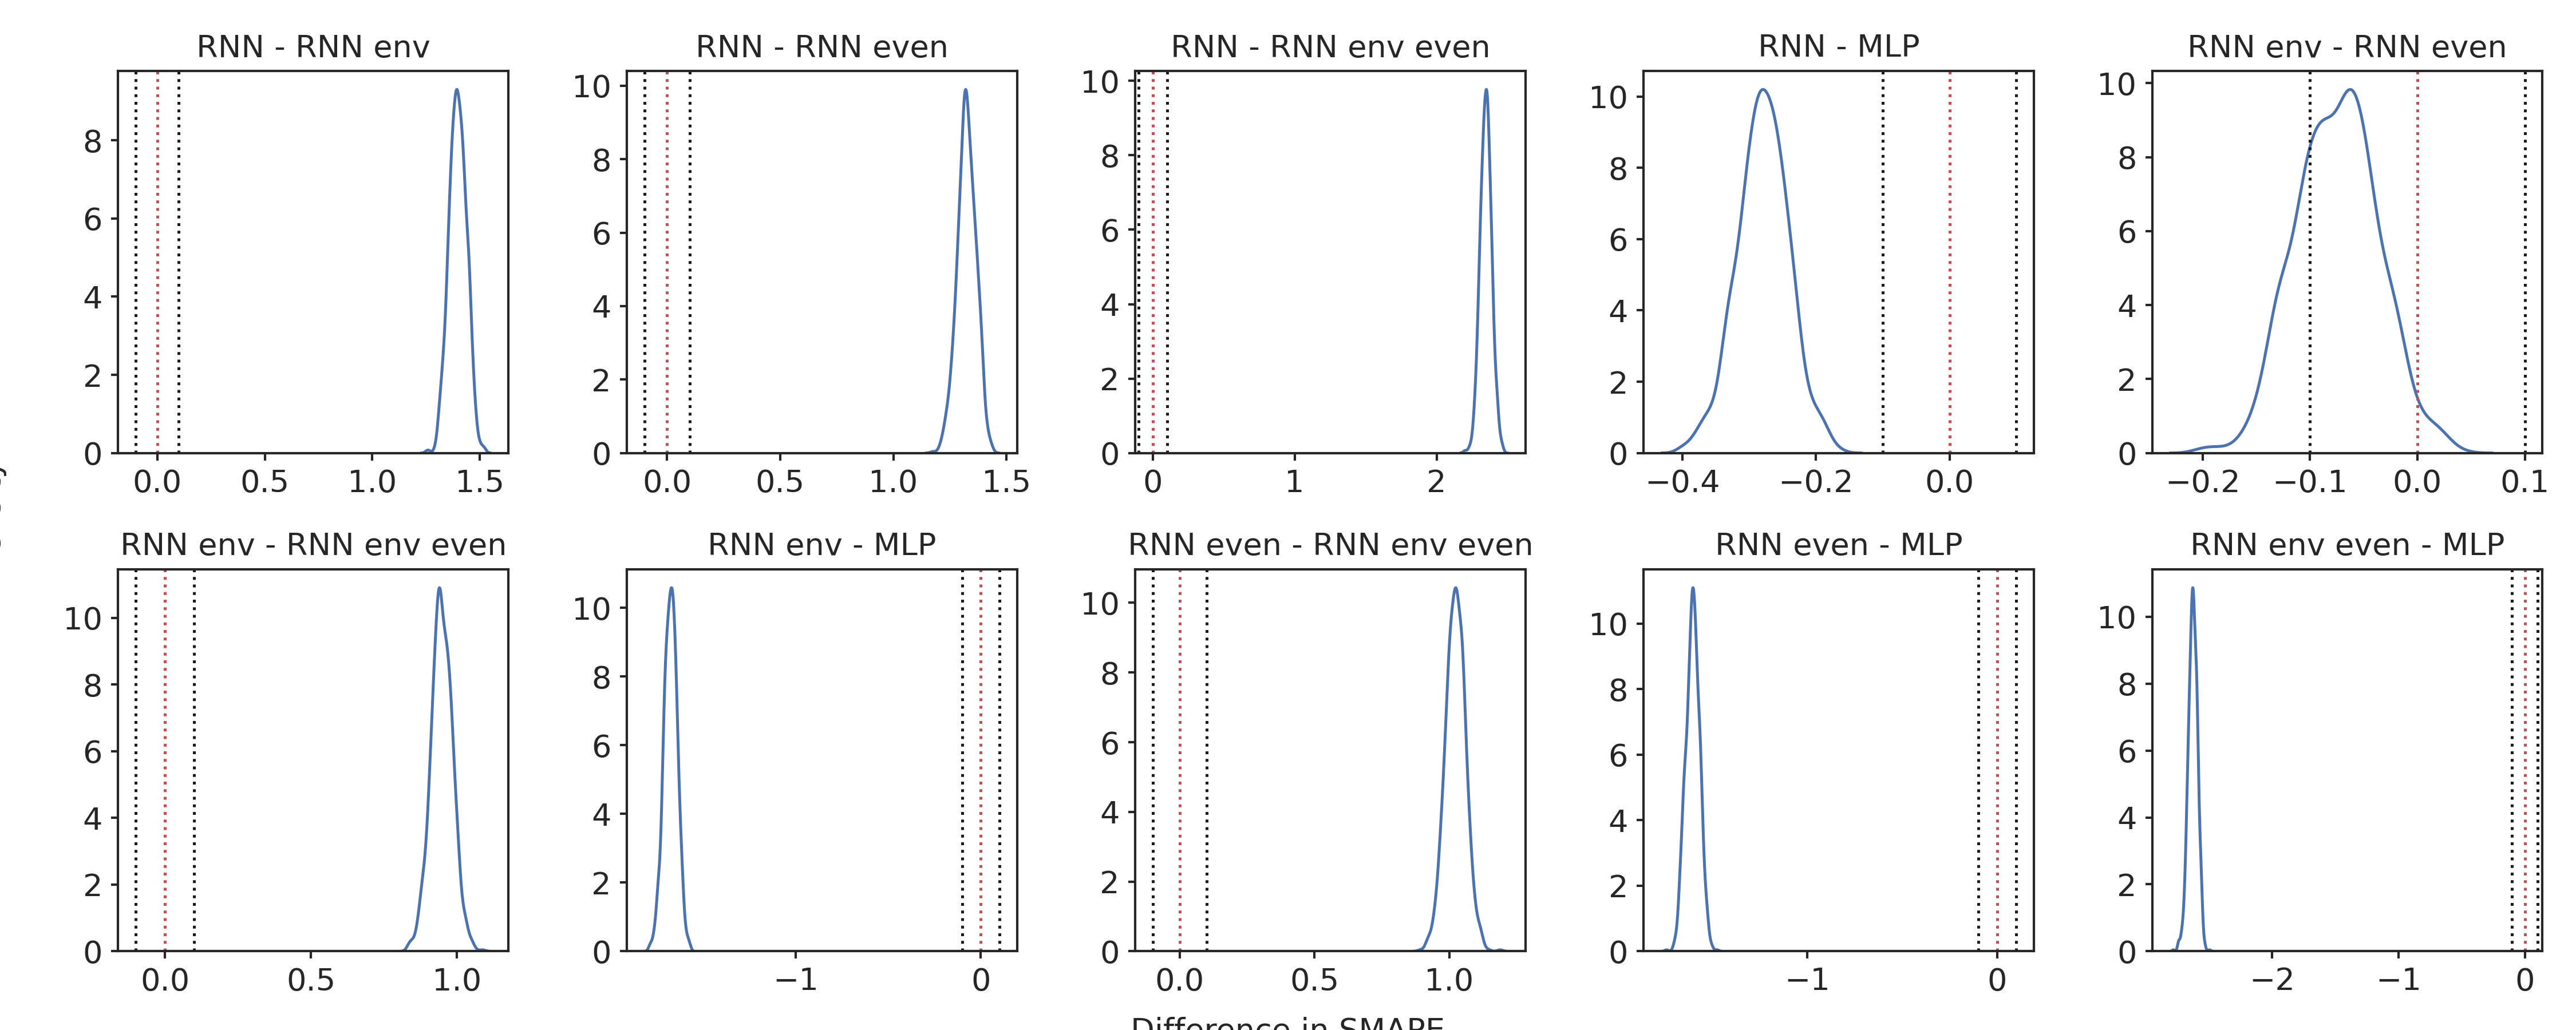
\includegraphics[width=\textwidth]{images/appendix_C/Future_Absence_comp_3.png}
\caption[\textbf{Future absence pairwise comparisons of model fixed effect}]{Pairwise comparisons of the parameter $\alpha$ (i.e. model slope) estimated by the model fitted for the Future Absence target.}
\label{comp_abs_3}
\end{figure} \FloatBarrier

\subsection{Future Active Time}
\label{future_abs_bayes_3}

\begin{figure}[ht]
\centering
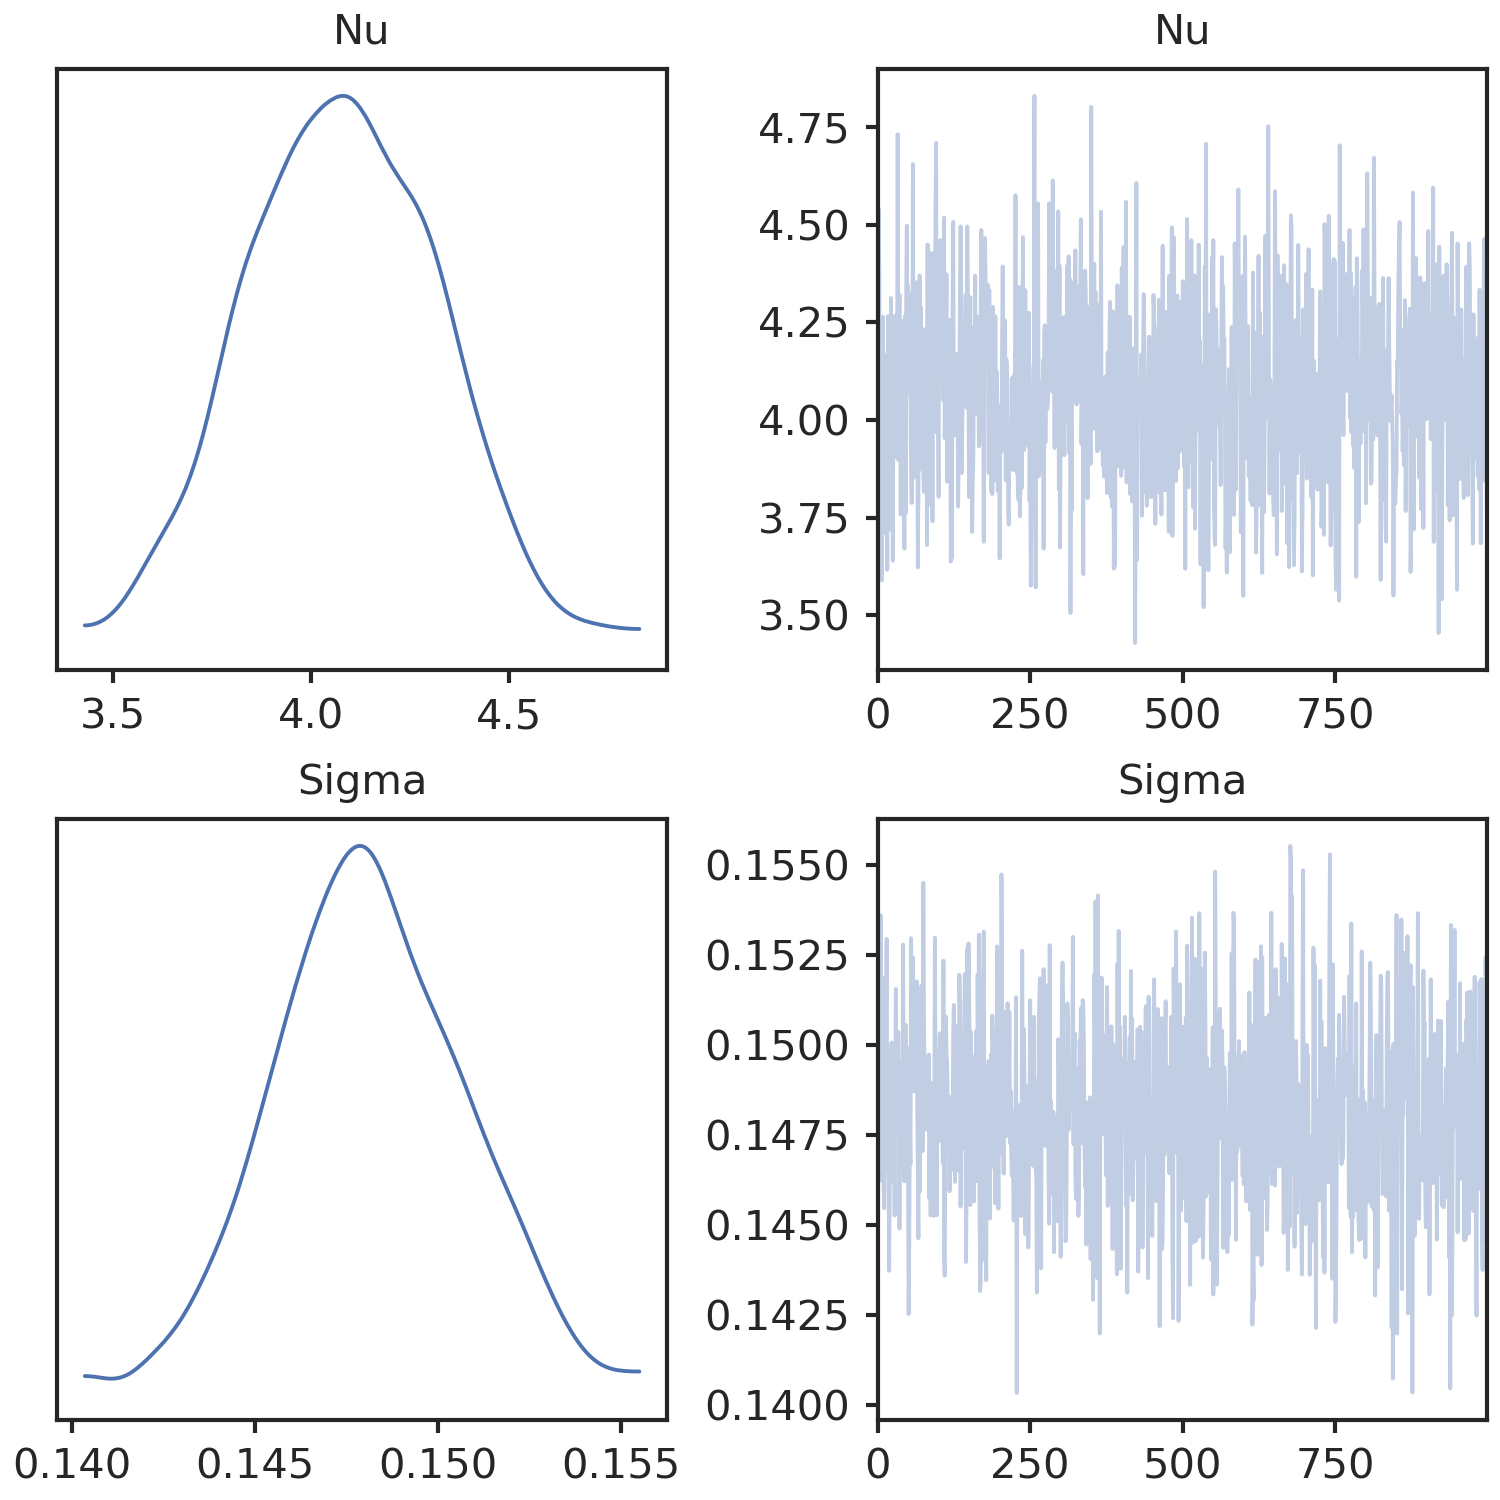
\includegraphics[width=0.5\textwidth]{images/appendix_C/Future Active Time_marginals_3.png}
\caption[\textbf{Future active time marginal distributions}]{Marginal distributions for the parameters $\nu$, $\sigma$ estimated by the model fitted for the Future Active Time target.}
\label{marginals_act_3}
\end{figure} \FloatBarrier

\begin{figure}[ht]
\centering
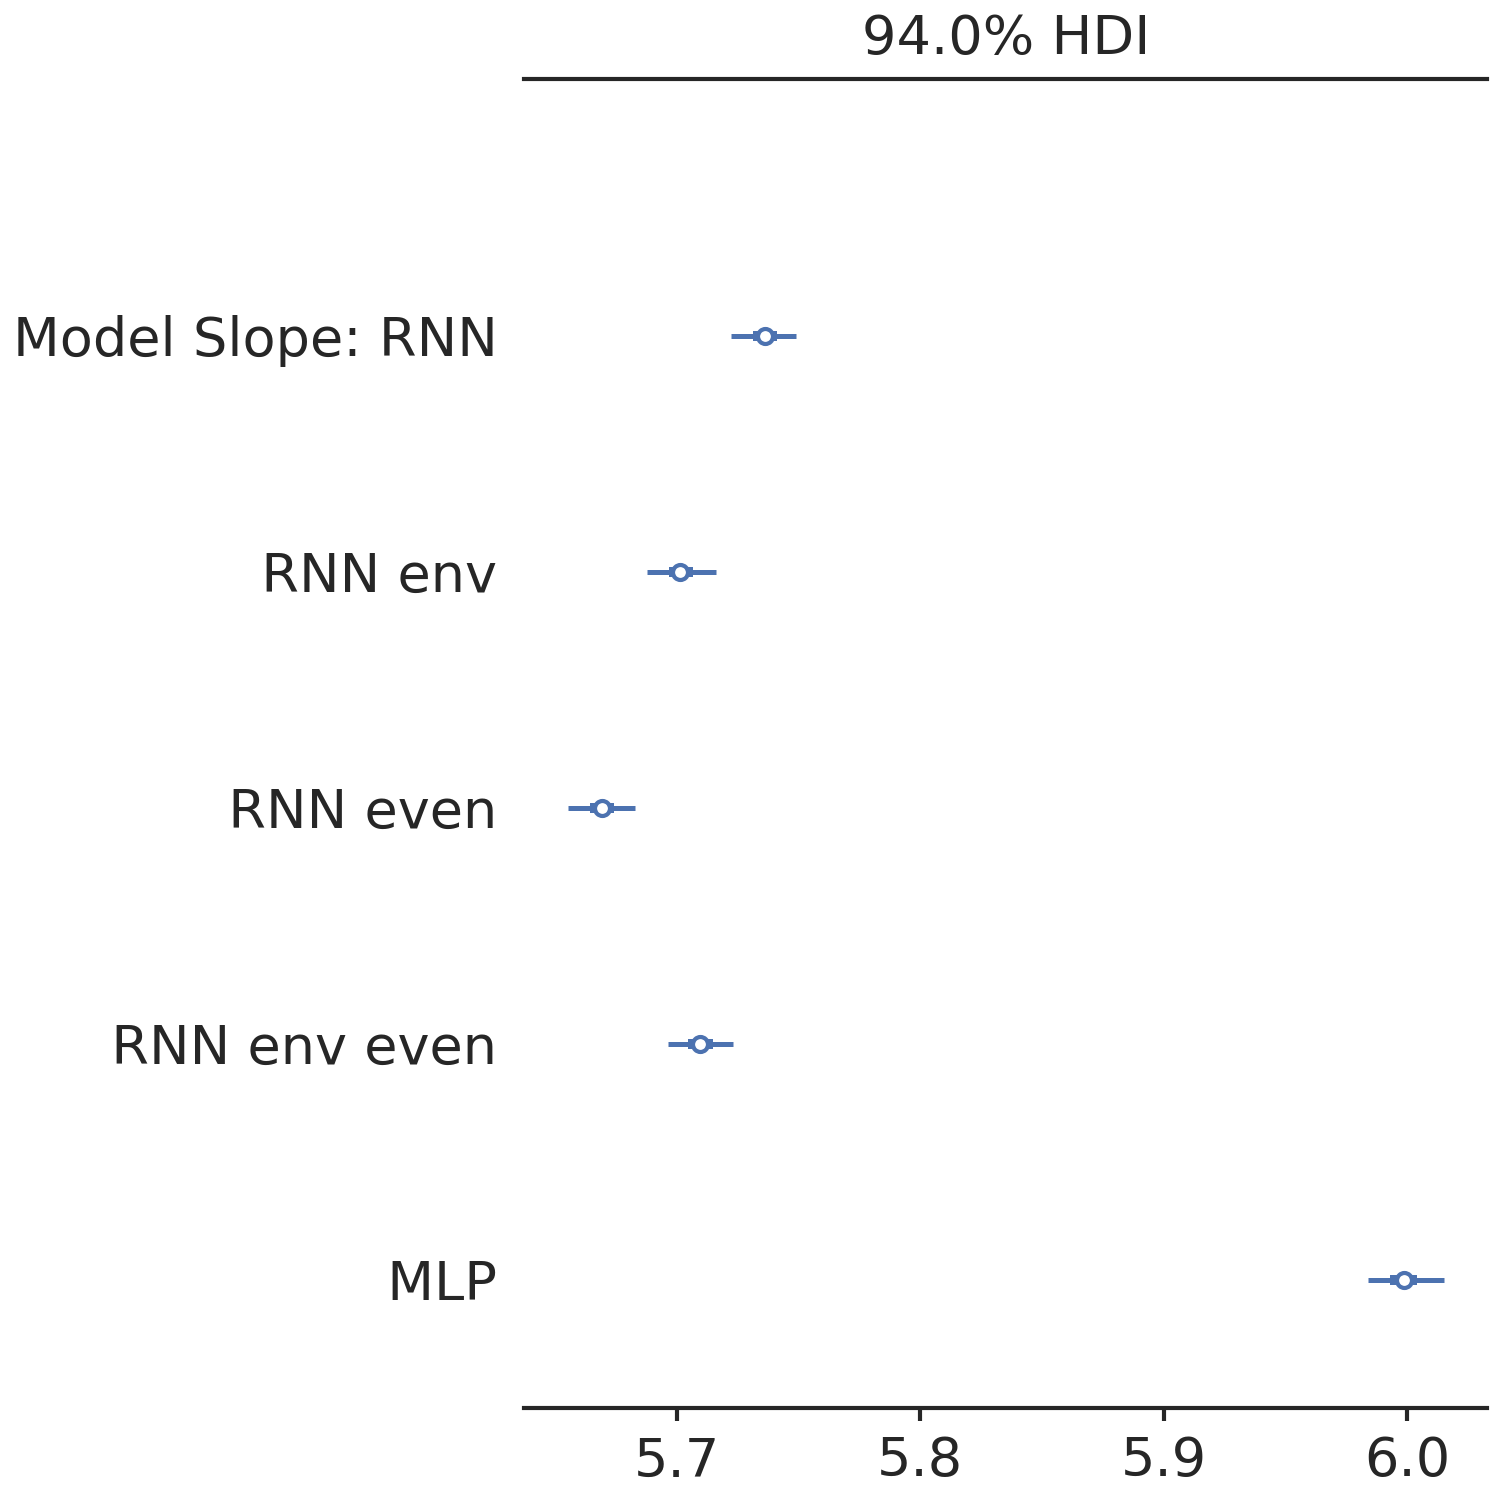
\includegraphics[width=0.5\textwidth]{images/appendix_C/Future Active Time_models_3.png}
\caption[\textbf{Future active time model fixed effect}]{Forest plot of the marginal distributions for the parameter $\alpha$ (i.e. model slope) estimated by the model fitted for the Future Active Time target.}
\label{model_act_3}
\end{figure} \FloatBarrier

\begin{figure}[ht]
\centering
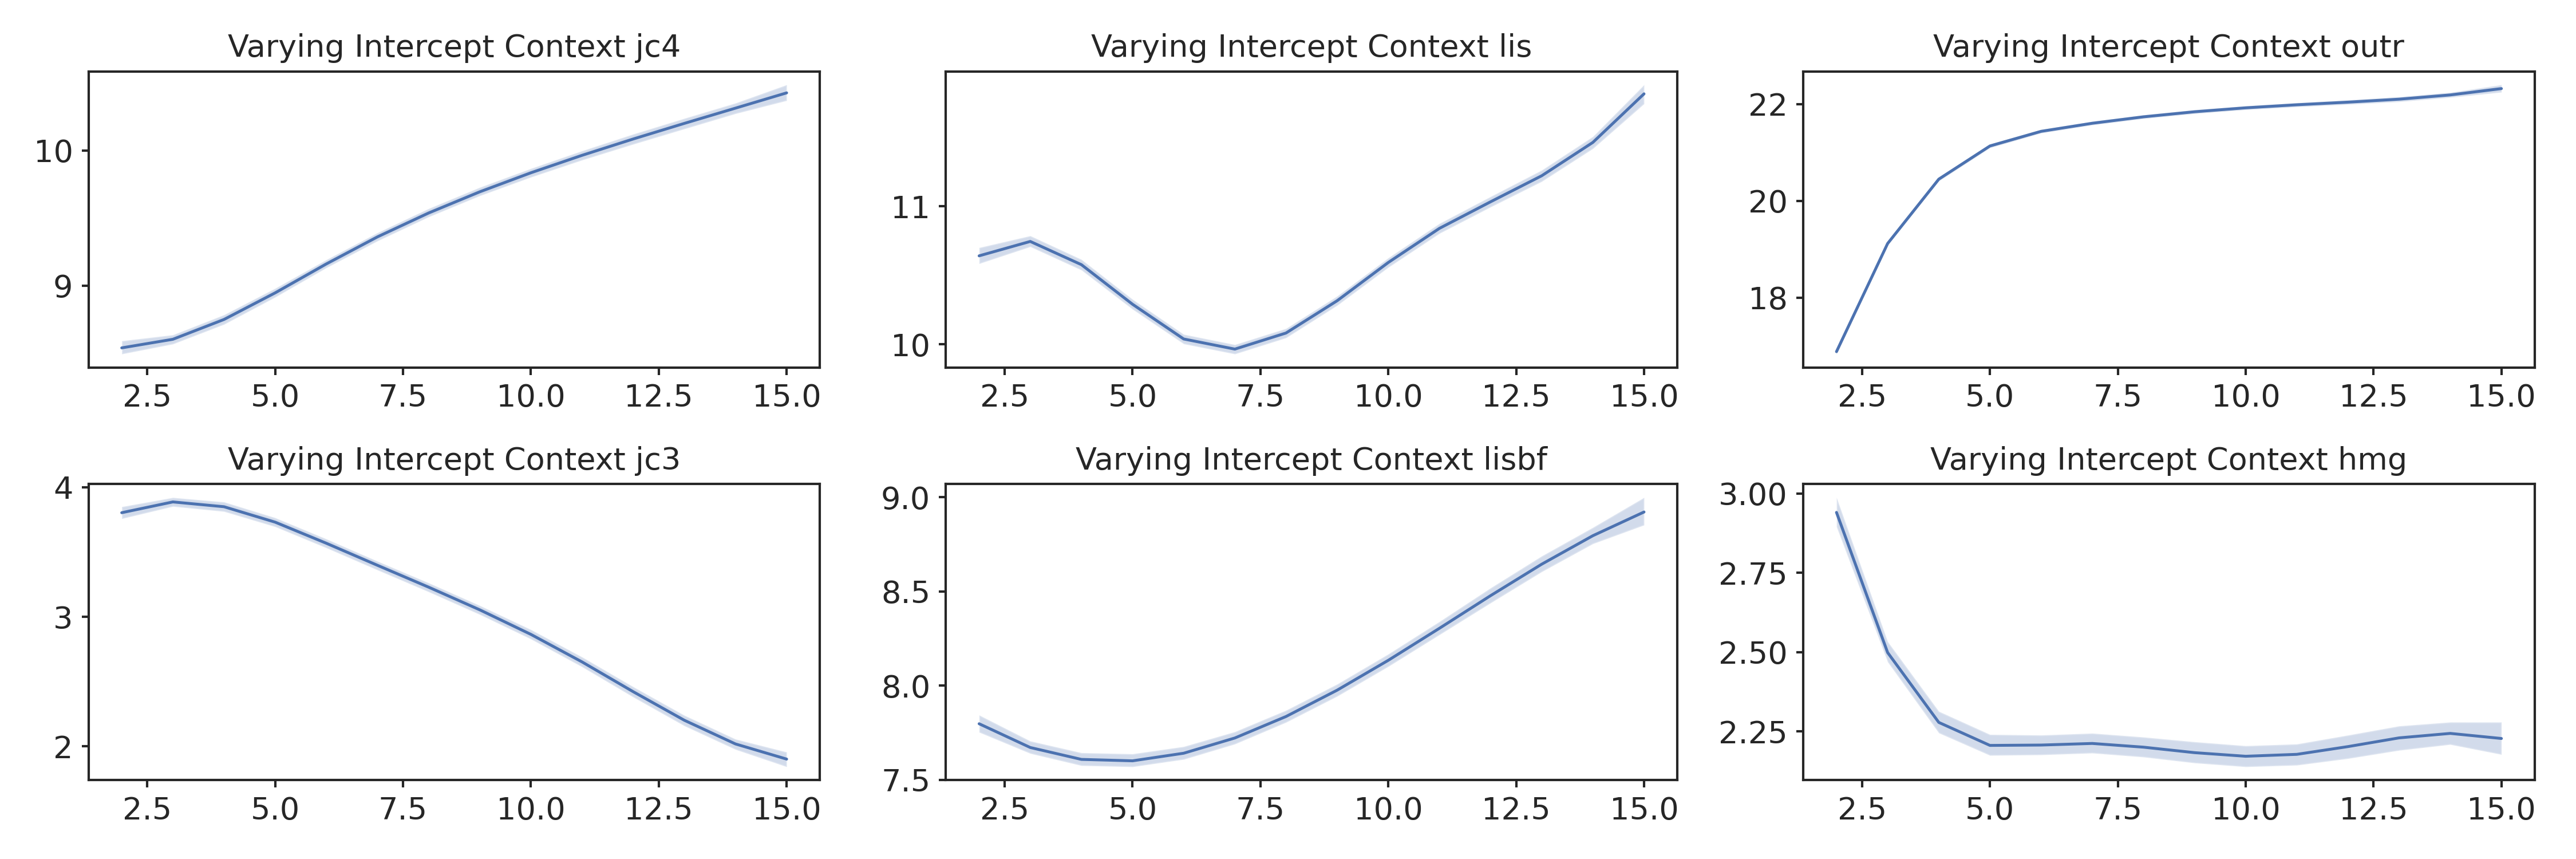
\includegraphics[width=\textwidth]{images/appendix_C/Future Active Time_interc_3.png}
\caption[\textbf{Future active time time-varying random intercept}]{Time varying random intercept estimated by the model fitted for the Future Active Time target.}
\label{interc_act_3}
\end{figure} \FloatBarrier

\begin{figure}[ht]
\centering
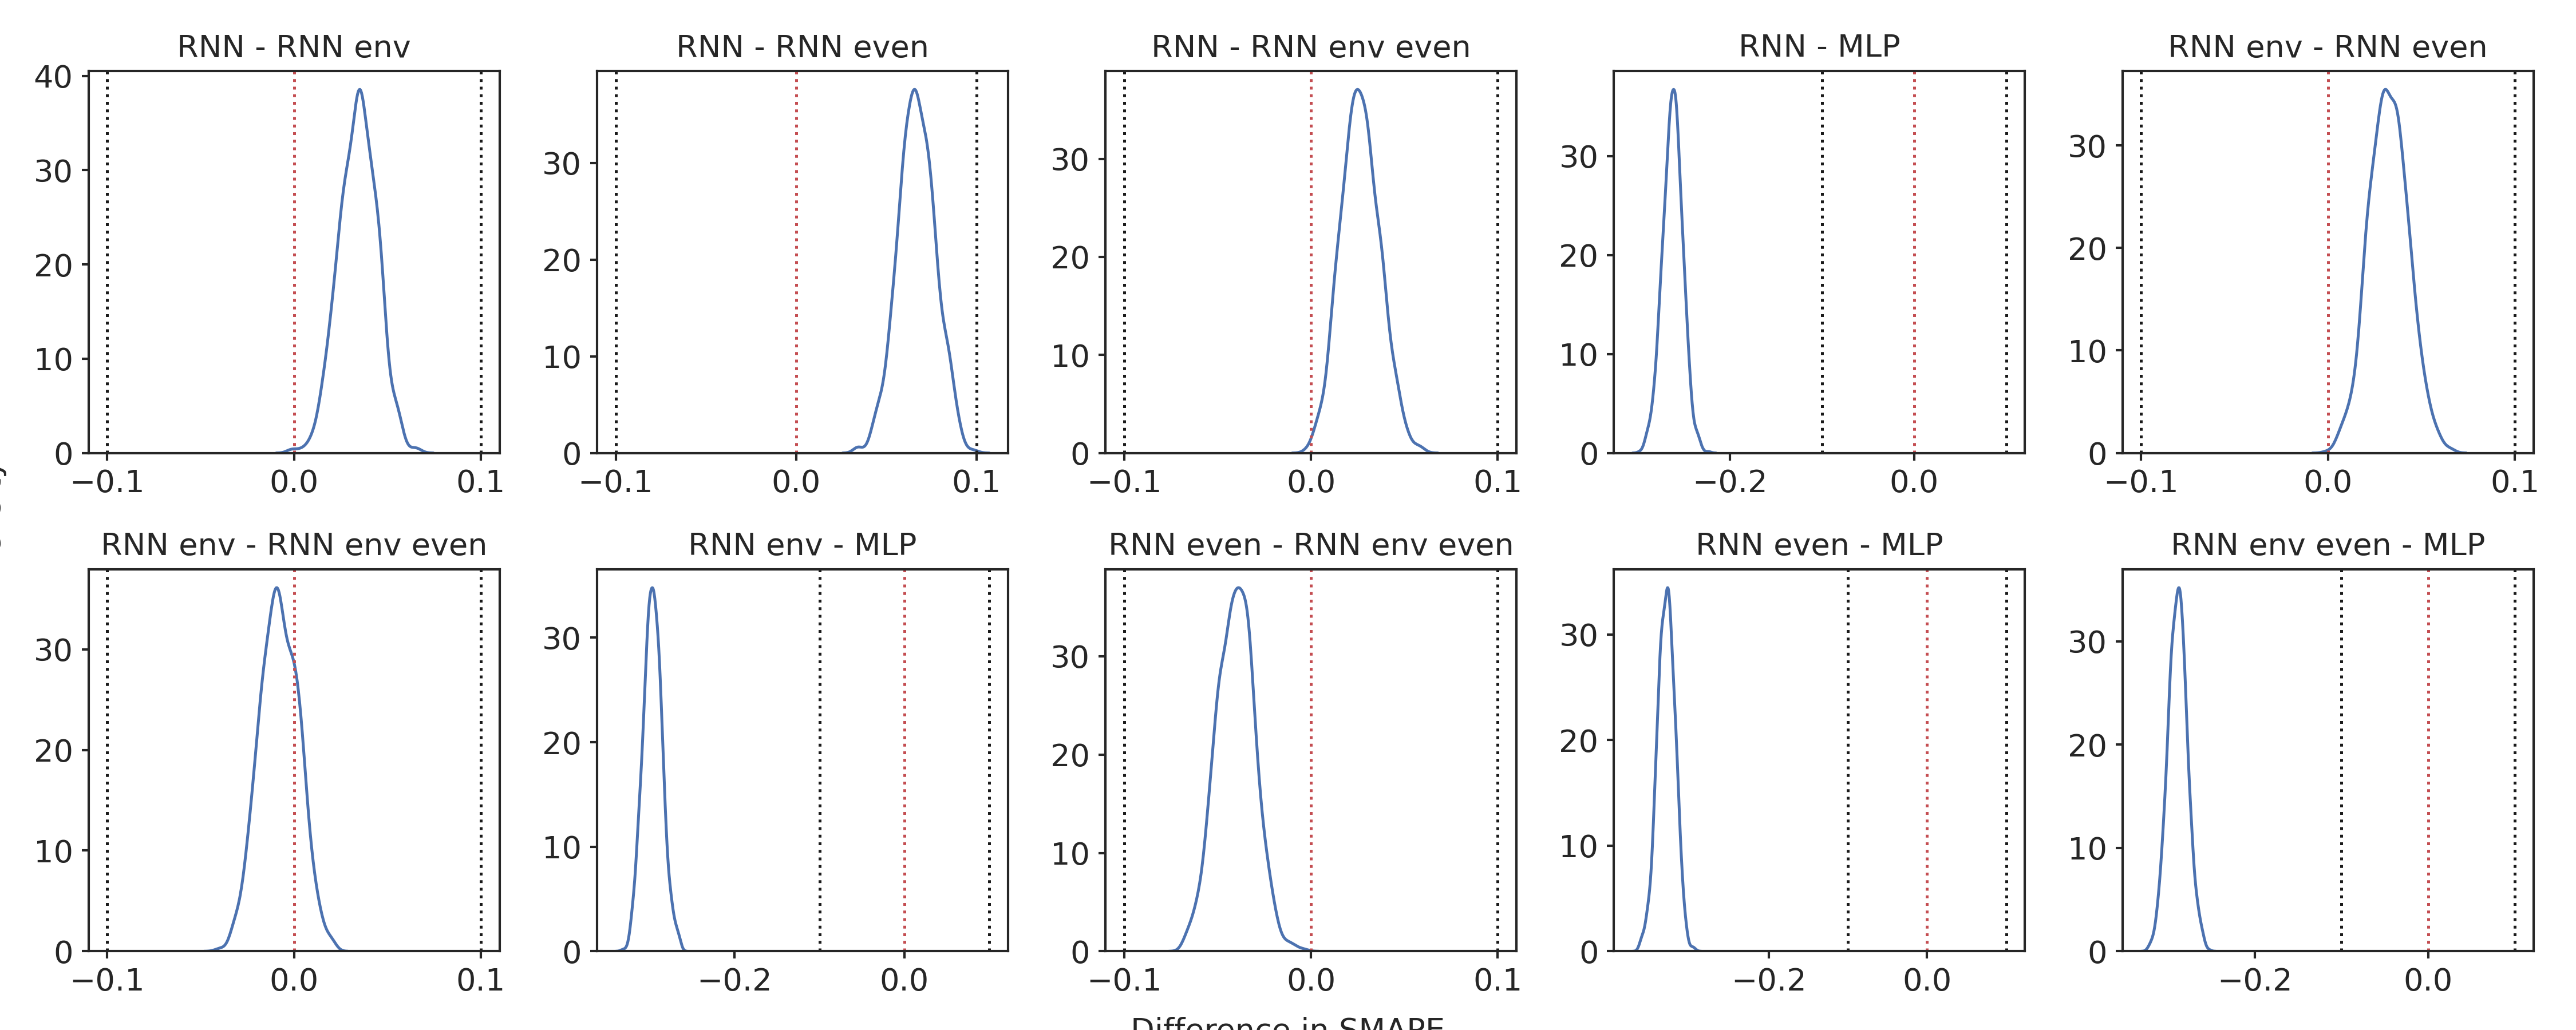
\includegraphics[width=\textwidth]{images/appendix_C/Future_Active_Time_comp_3.png}
\caption[\textbf{Future active time pairwise comparisons of model fixed effect}]{Pairwise comparisons of the parameter $\alpha$ (i.e. model slope) estimated by the model fitted for the Future Active Time target.}
\label{comp_act_3}
\end{figure} \FloatBarrier

\subsection{Future Session Time}
\label{future_sess_bayes_3}

\begin{figure}[ht]
\centering
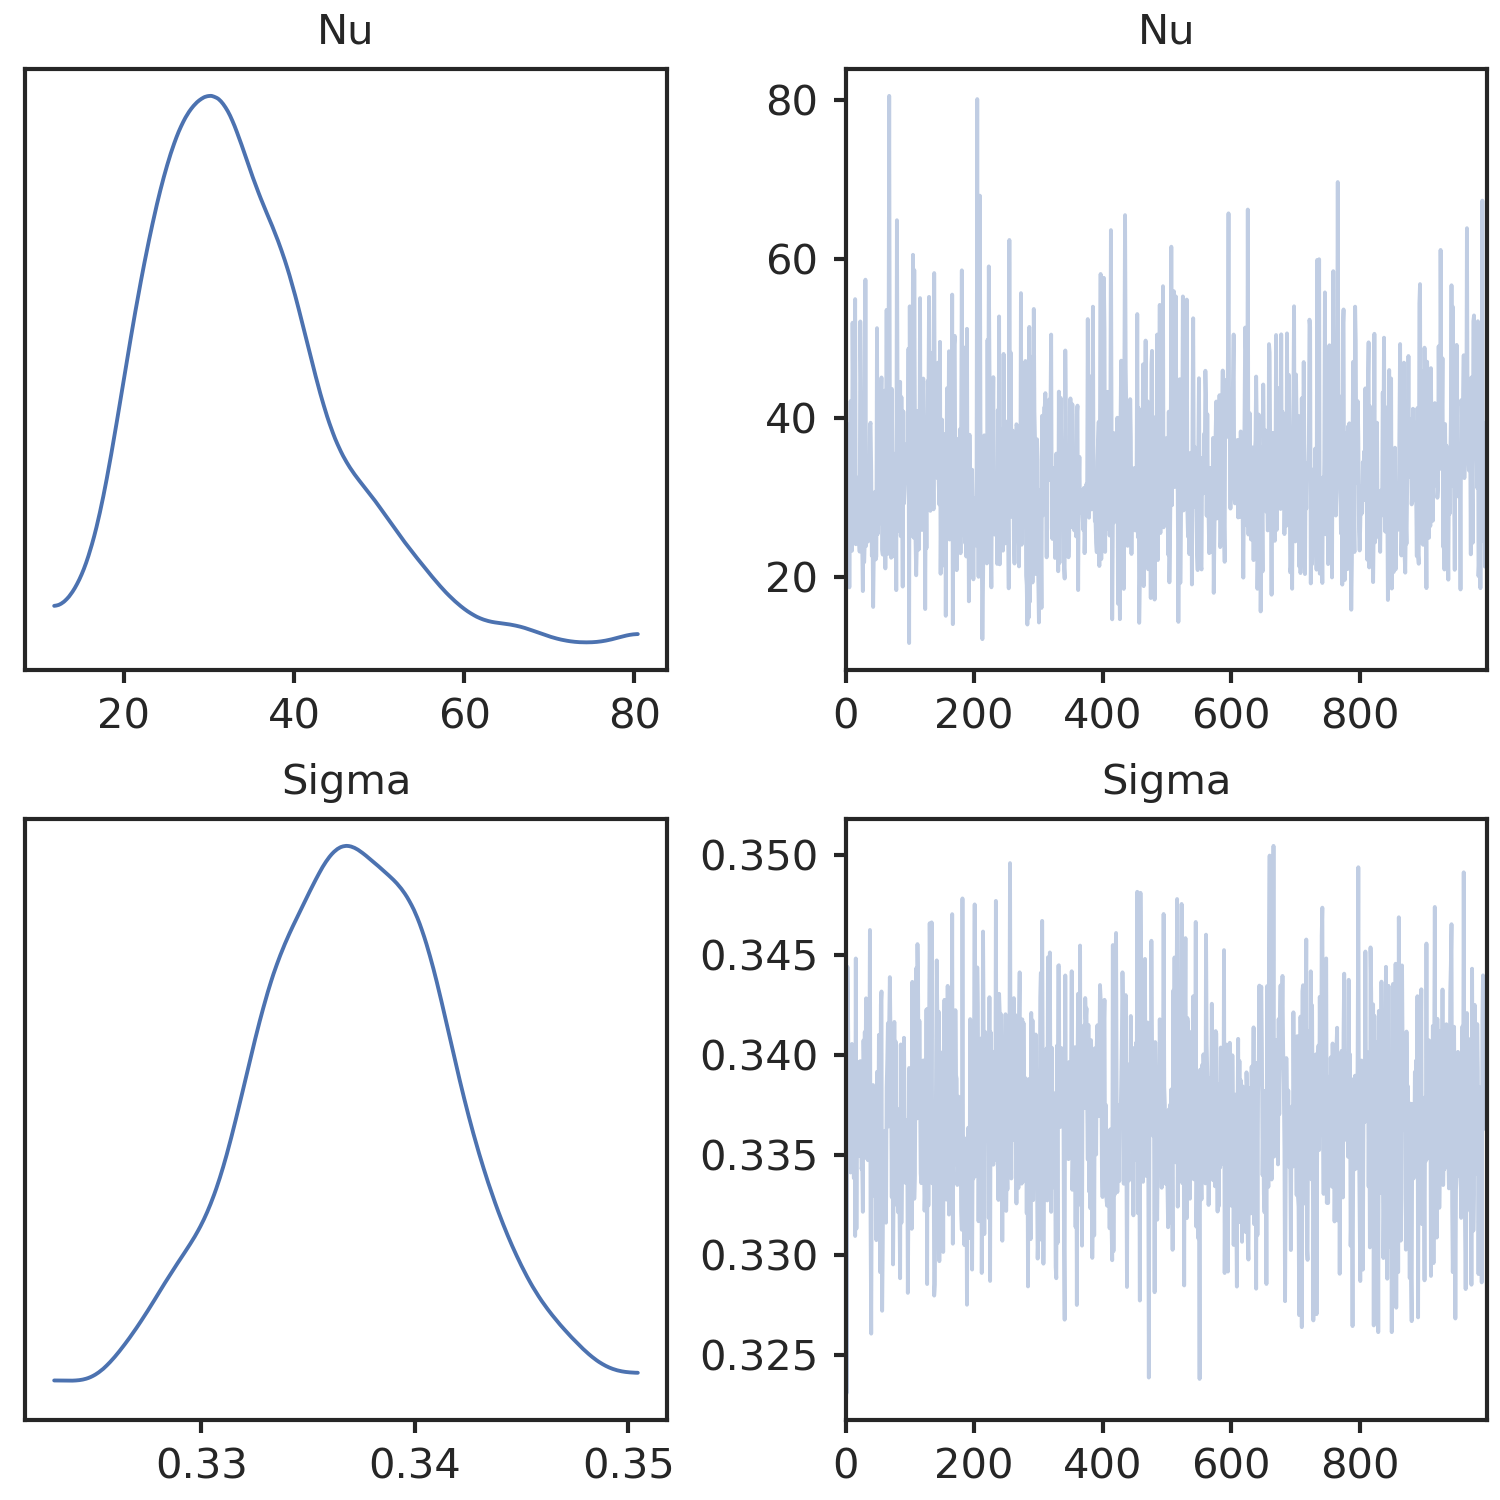
\includegraphics[width=0.5\textwidth]{images/appendix_C/Future Session Time_marginals_3.png}
\caption[\textbf{Future session time marginal distributions}]{Marginal distributions for the parameters $\nu$, $\sigma$ estimated by the model fitted for the Future Session Time target.}
\label{marginals_sess_3}
\end{figure} \FloatBarrier

\begin{figure}[ht]
\centering
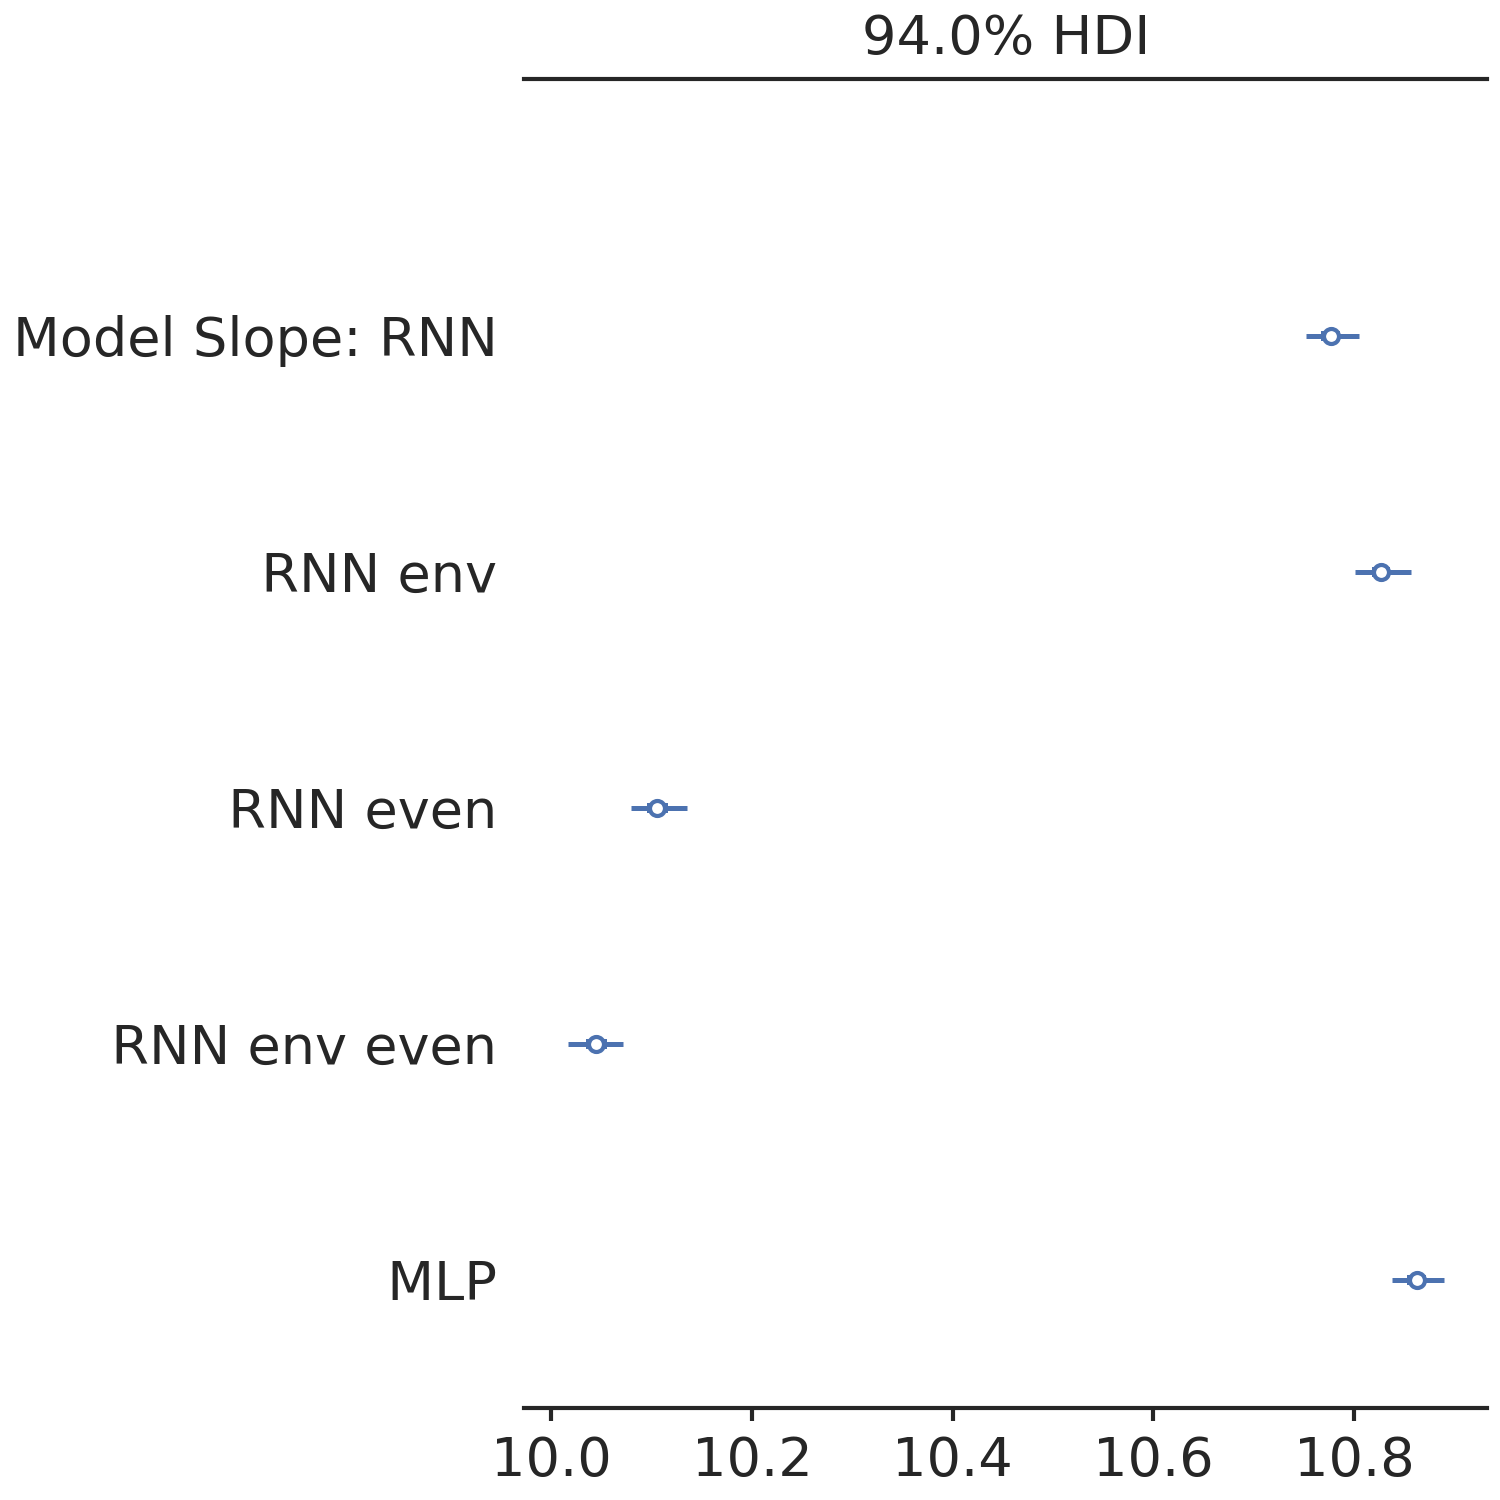
\includegraphics[width=0.5\textwidth]{images/appendix_C/Future Session Time_models_3.png}
\caption[\textbf{Future session time model fixed effect}]{Forest plot of the marginal distributions for the parameter $\alpha$ (i.e. model slope) estimated by the model fitted for the Future Session Time target.}
\label{model_sess_3}
\end{figure} \FloatBarrier

\begin{figure}[ht]
\centering
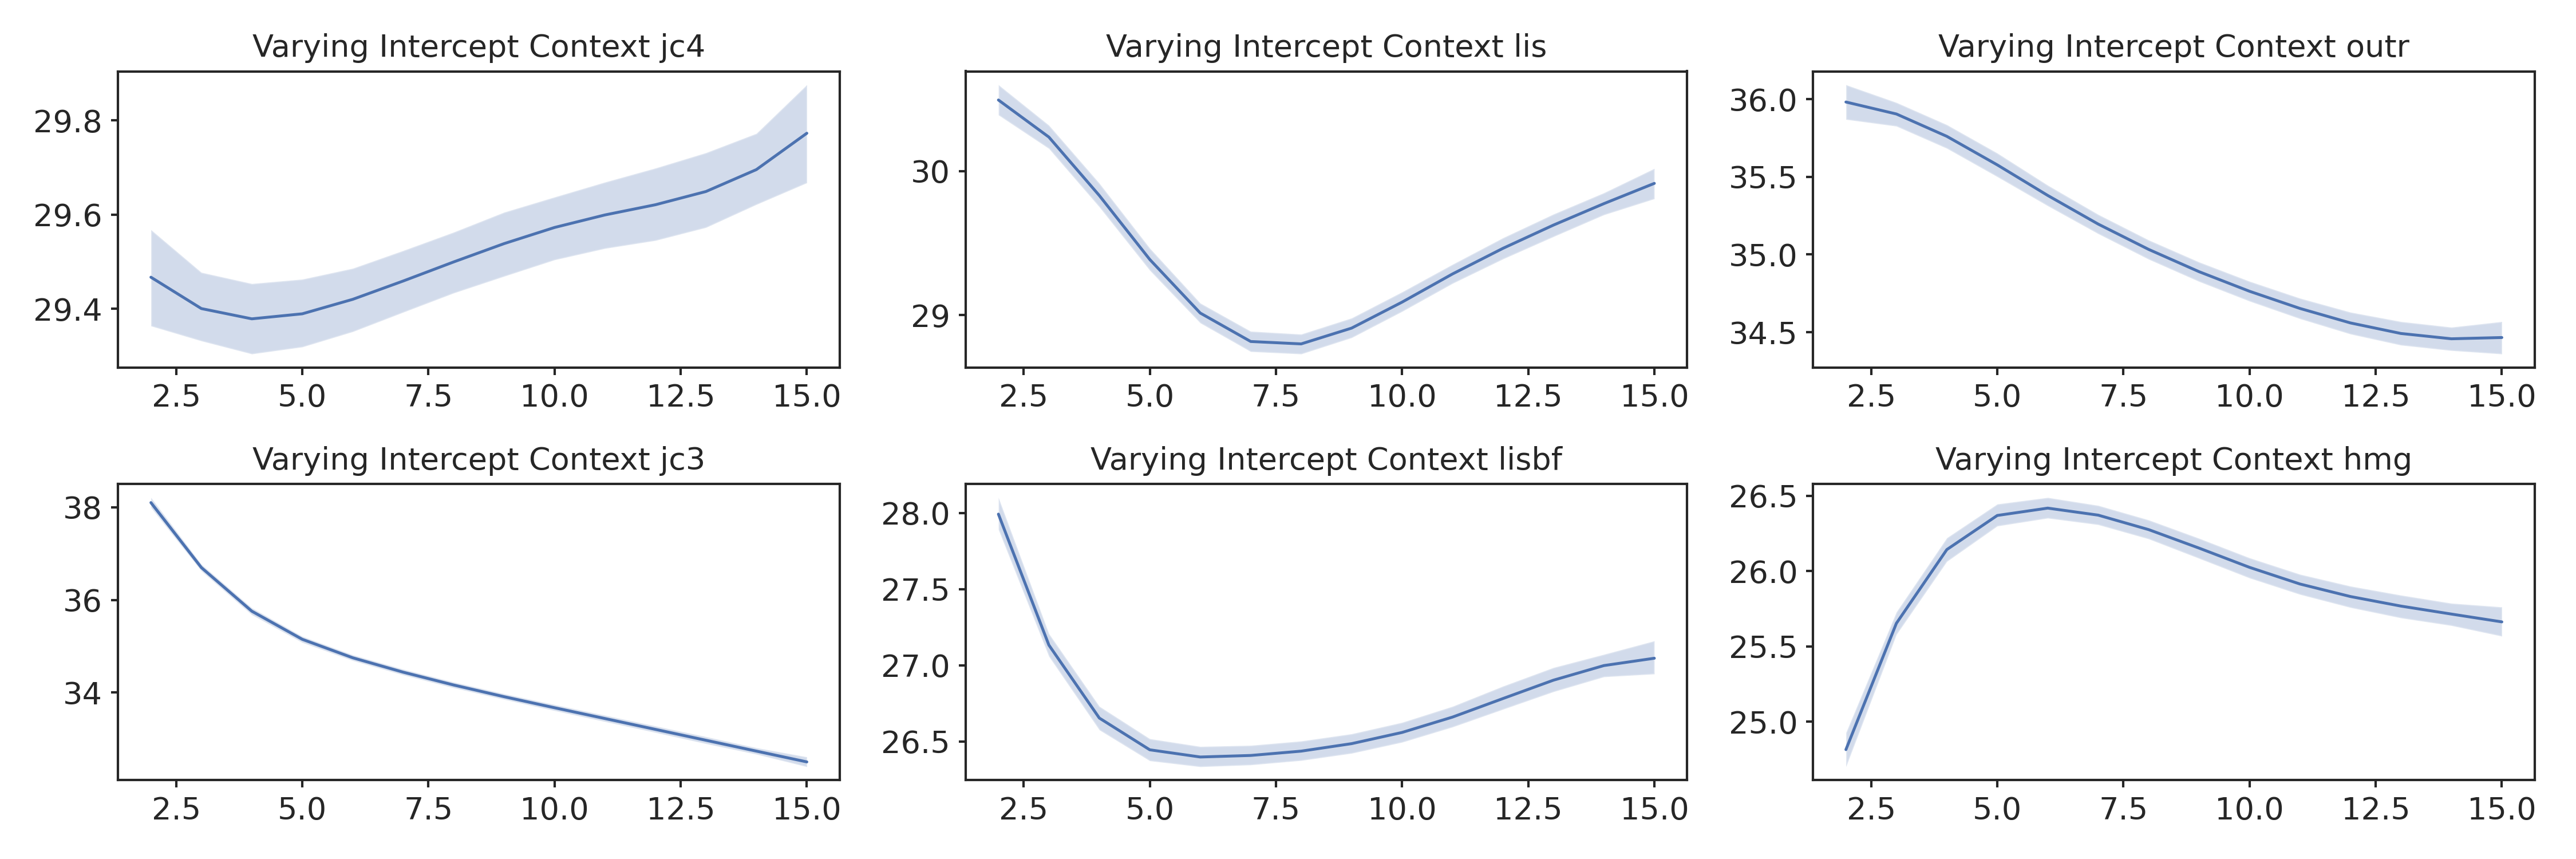
\includegraphics[width=\textwidth]{images/appendix_C/Future Session Time_interc_3.png}
\caption[\textbf{Future session time time-varying random intercept}]{Time varying random intercept estimated by the model fitted for the Future Session Time target.}
\label{interc_sess_3}
\end{figure} \FloatBarrier

\begin{figure}[ht]
\centering
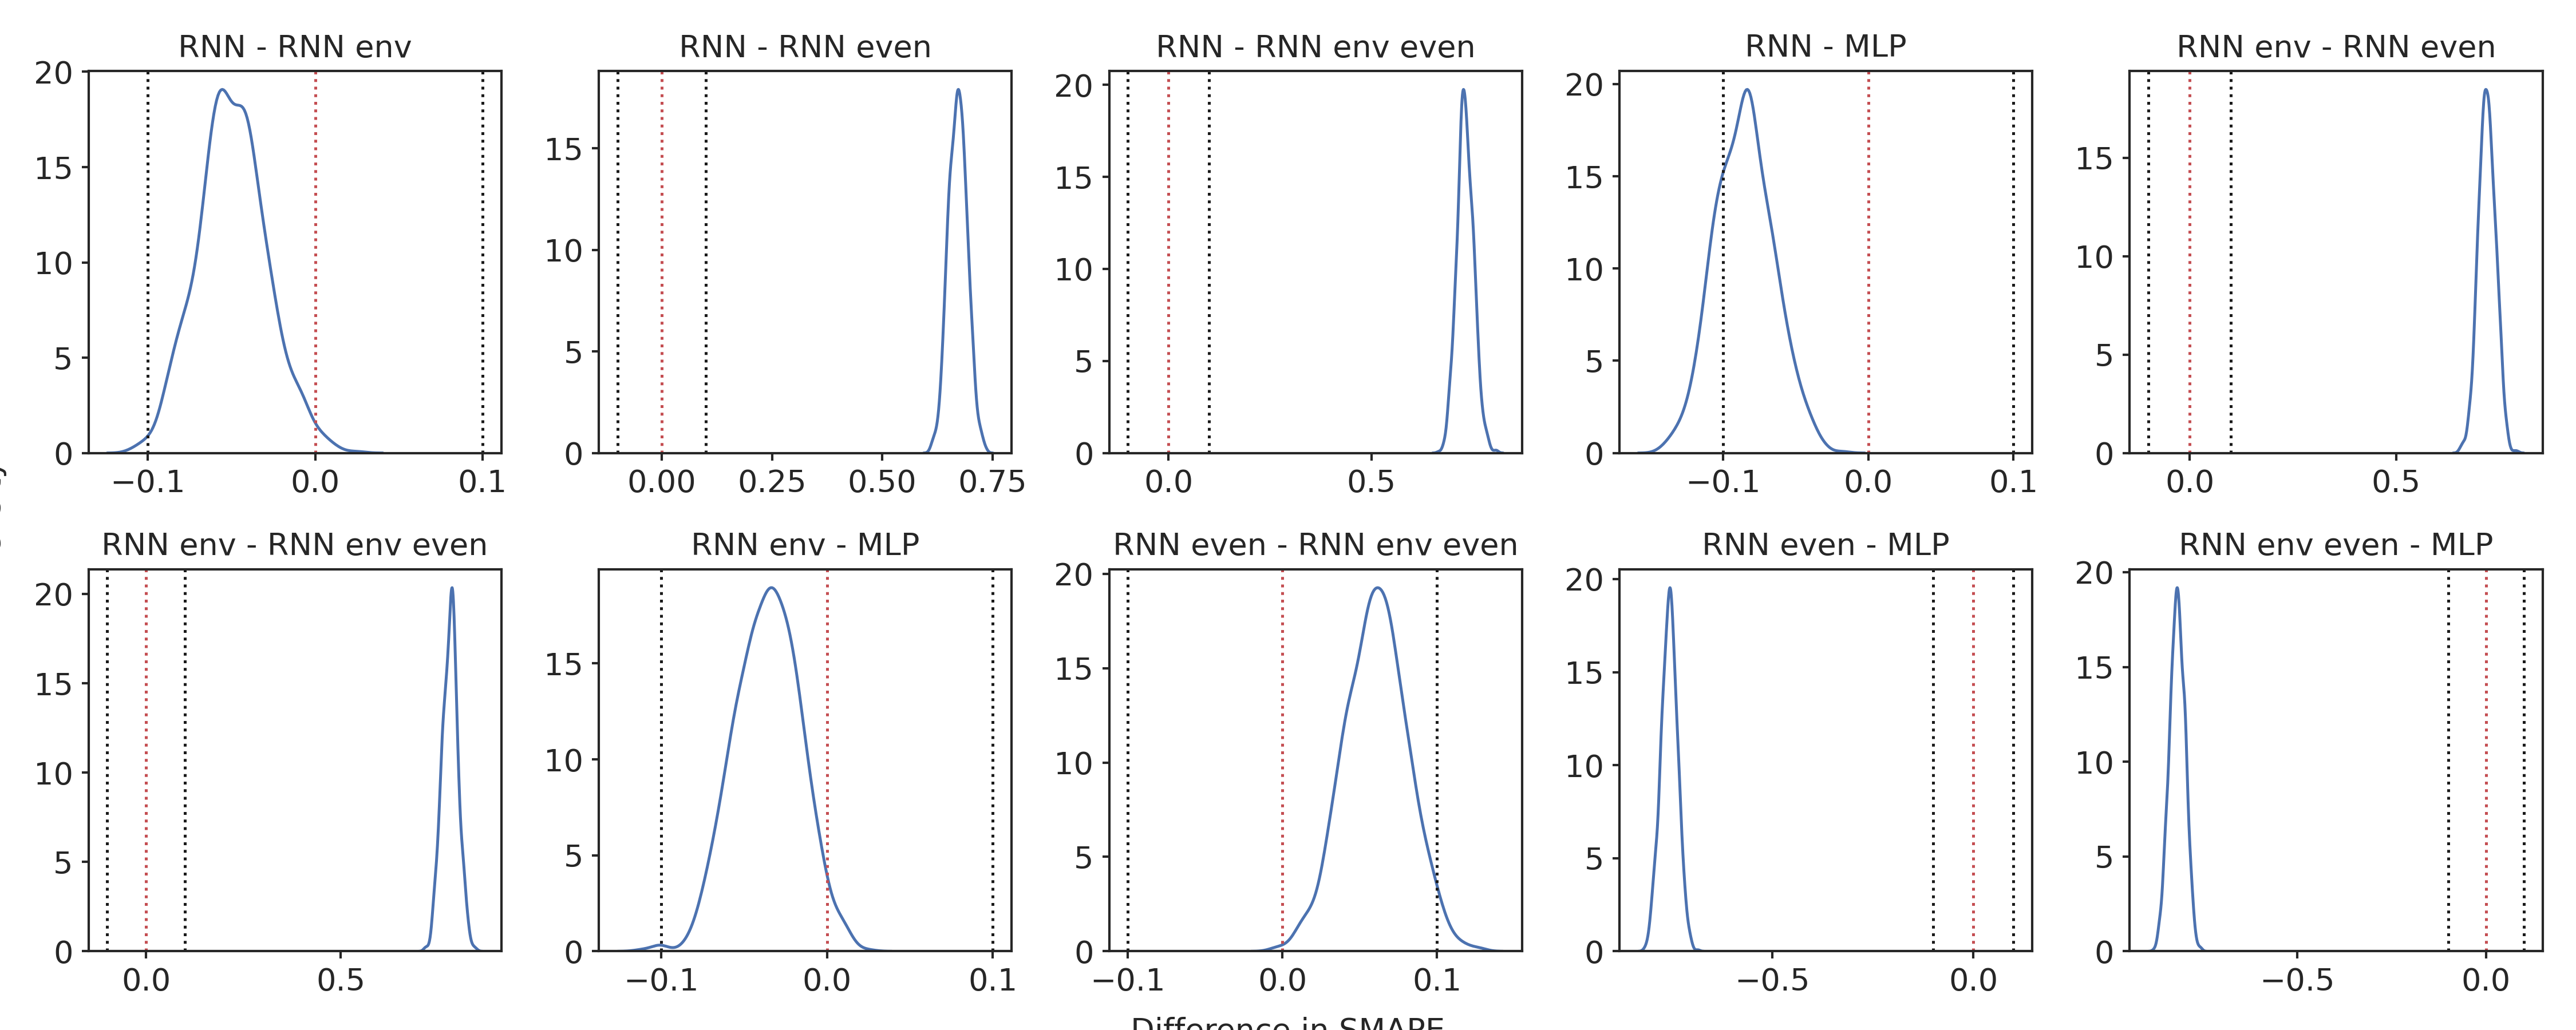
\includegraphics[width=\textwidth]{images/appendix_C/Future_Session_Time_comp_3.png}
\caption[\textbf{Future session time pairwise comparisons of model fixed effect}]{Pairwise comparisons of the parameter $\alpha$ (i.e. model slope) estimated by the model fitted for the Future Session Time target.}
\label{comp_sess_3}
\end{figure} \FloatBarrier

\subsection{Future Session Activity}
\label{future_acti_bayes_3}

\begin{figure}[ht]
\centering
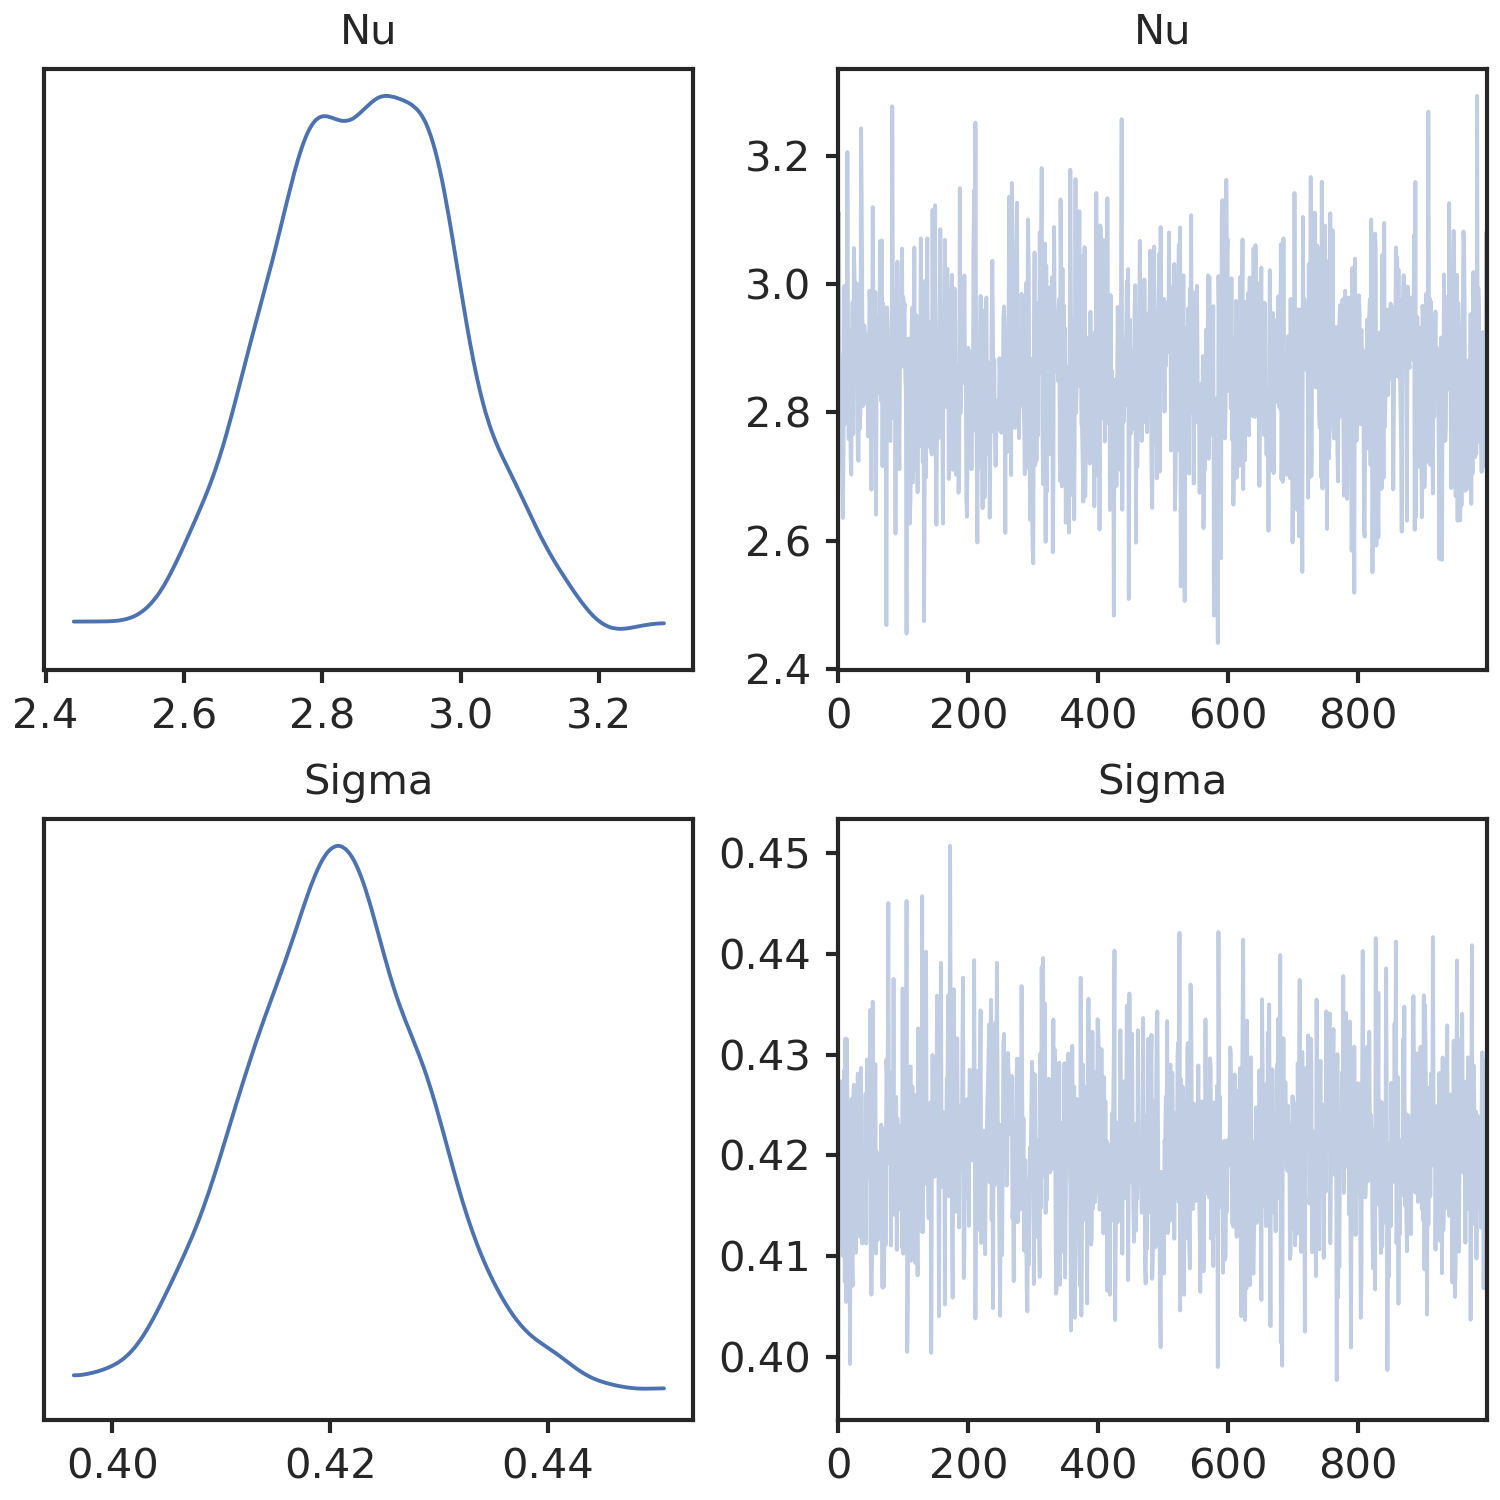
\includegraphics[width=0.5\textwidth]{images/appendix_C/Future Session Activity_marginals_3.png}
\caption[\textbf{Future session activity marginal distributions}]{Marginal distributions for the parameters $\nu$, $\sigma$ estimated by the model fitted for the Future Session Activity target.}
\label{marginals_acti_3}
\end{figure} \FloatBarrier

\begin{figure}[ht]
\centering
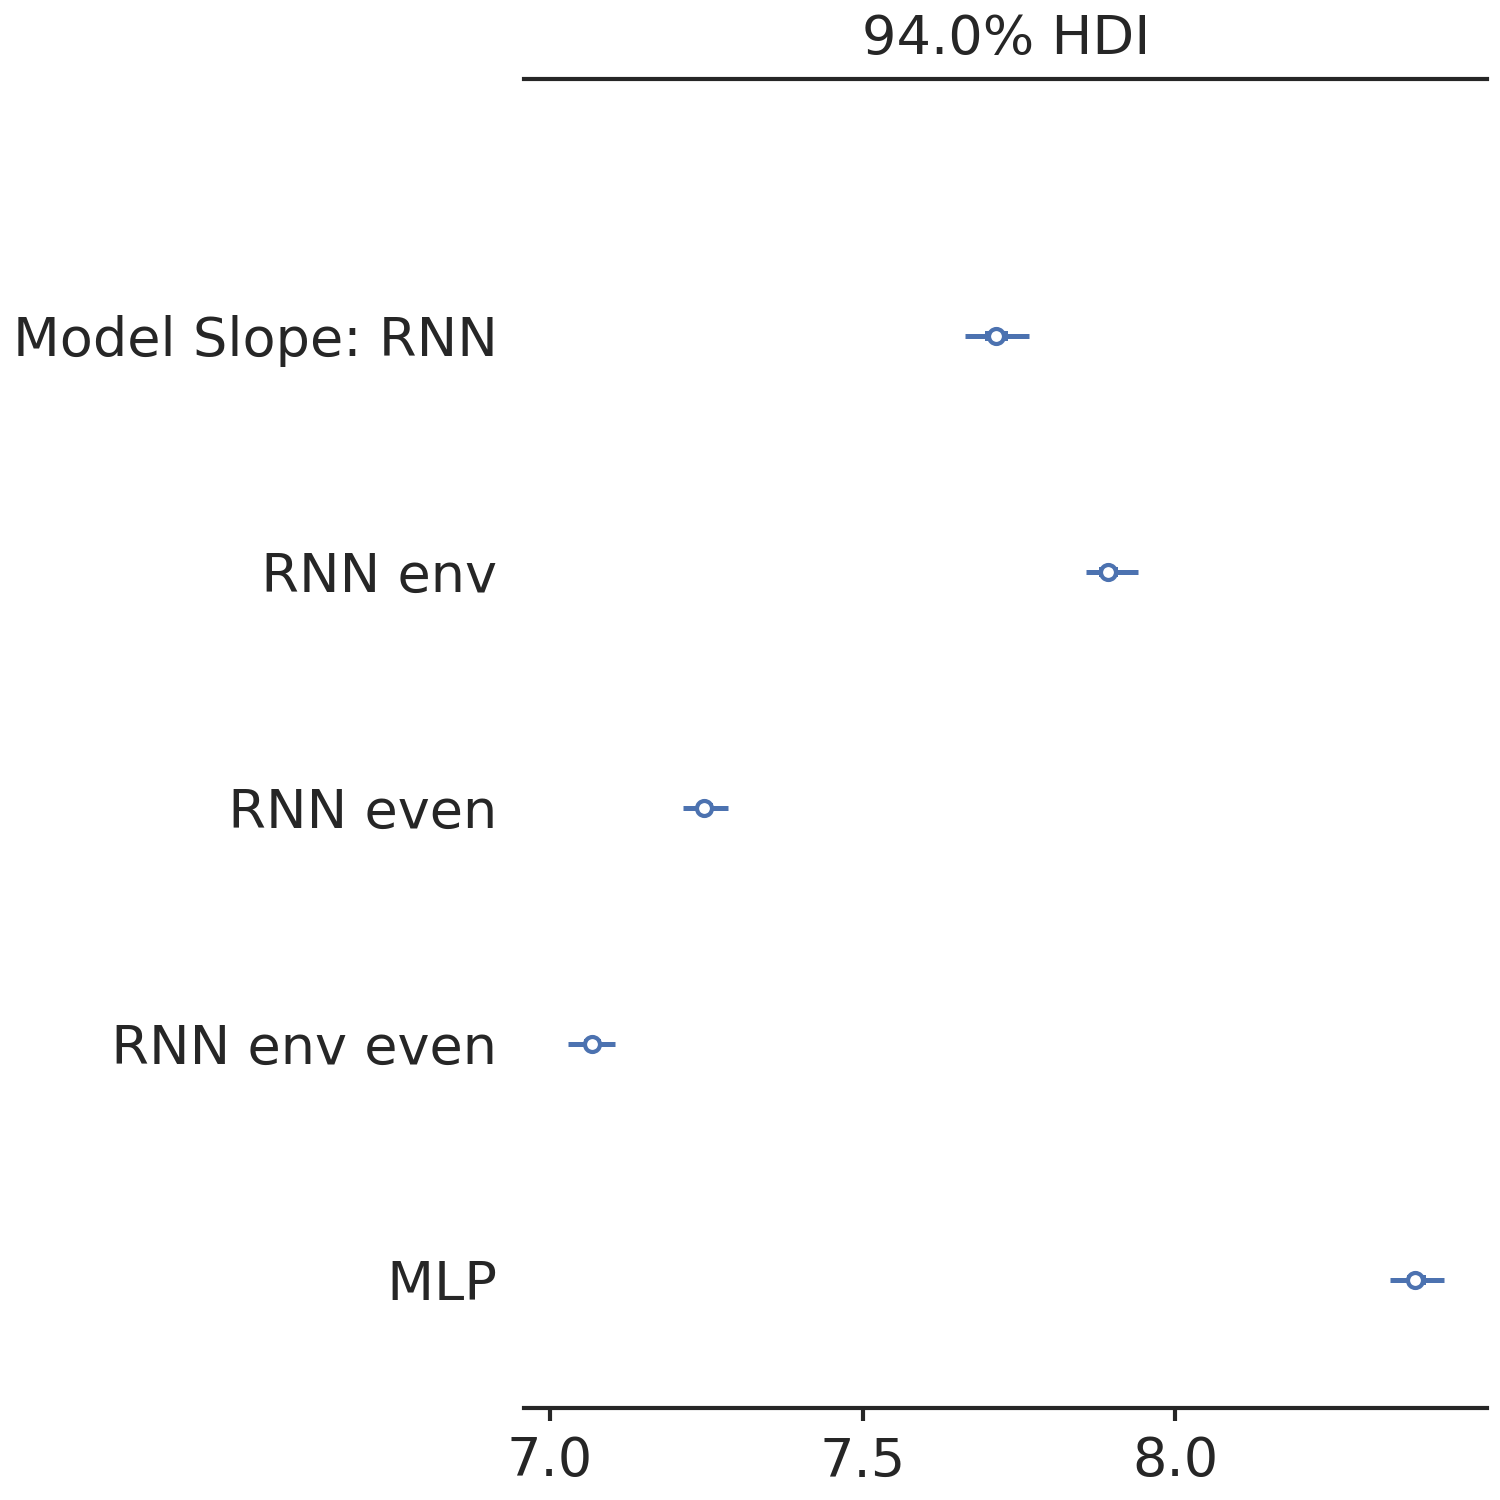
\includegraphics[width=0.5\textwidth]{images/appendix_C/Future Session Activity_models_3.png}
\caption[\textbf{Future session activity model fixed effect}]{Forest plot of the marginal distributions for the parameter $\alpha$ (i.e. model slope) estimated by the model fitted for the Future Session Activity target.}
\label{model_acti_3}
\end{figure} \FloatBarrier

\begin{figure}[ht]
\centering
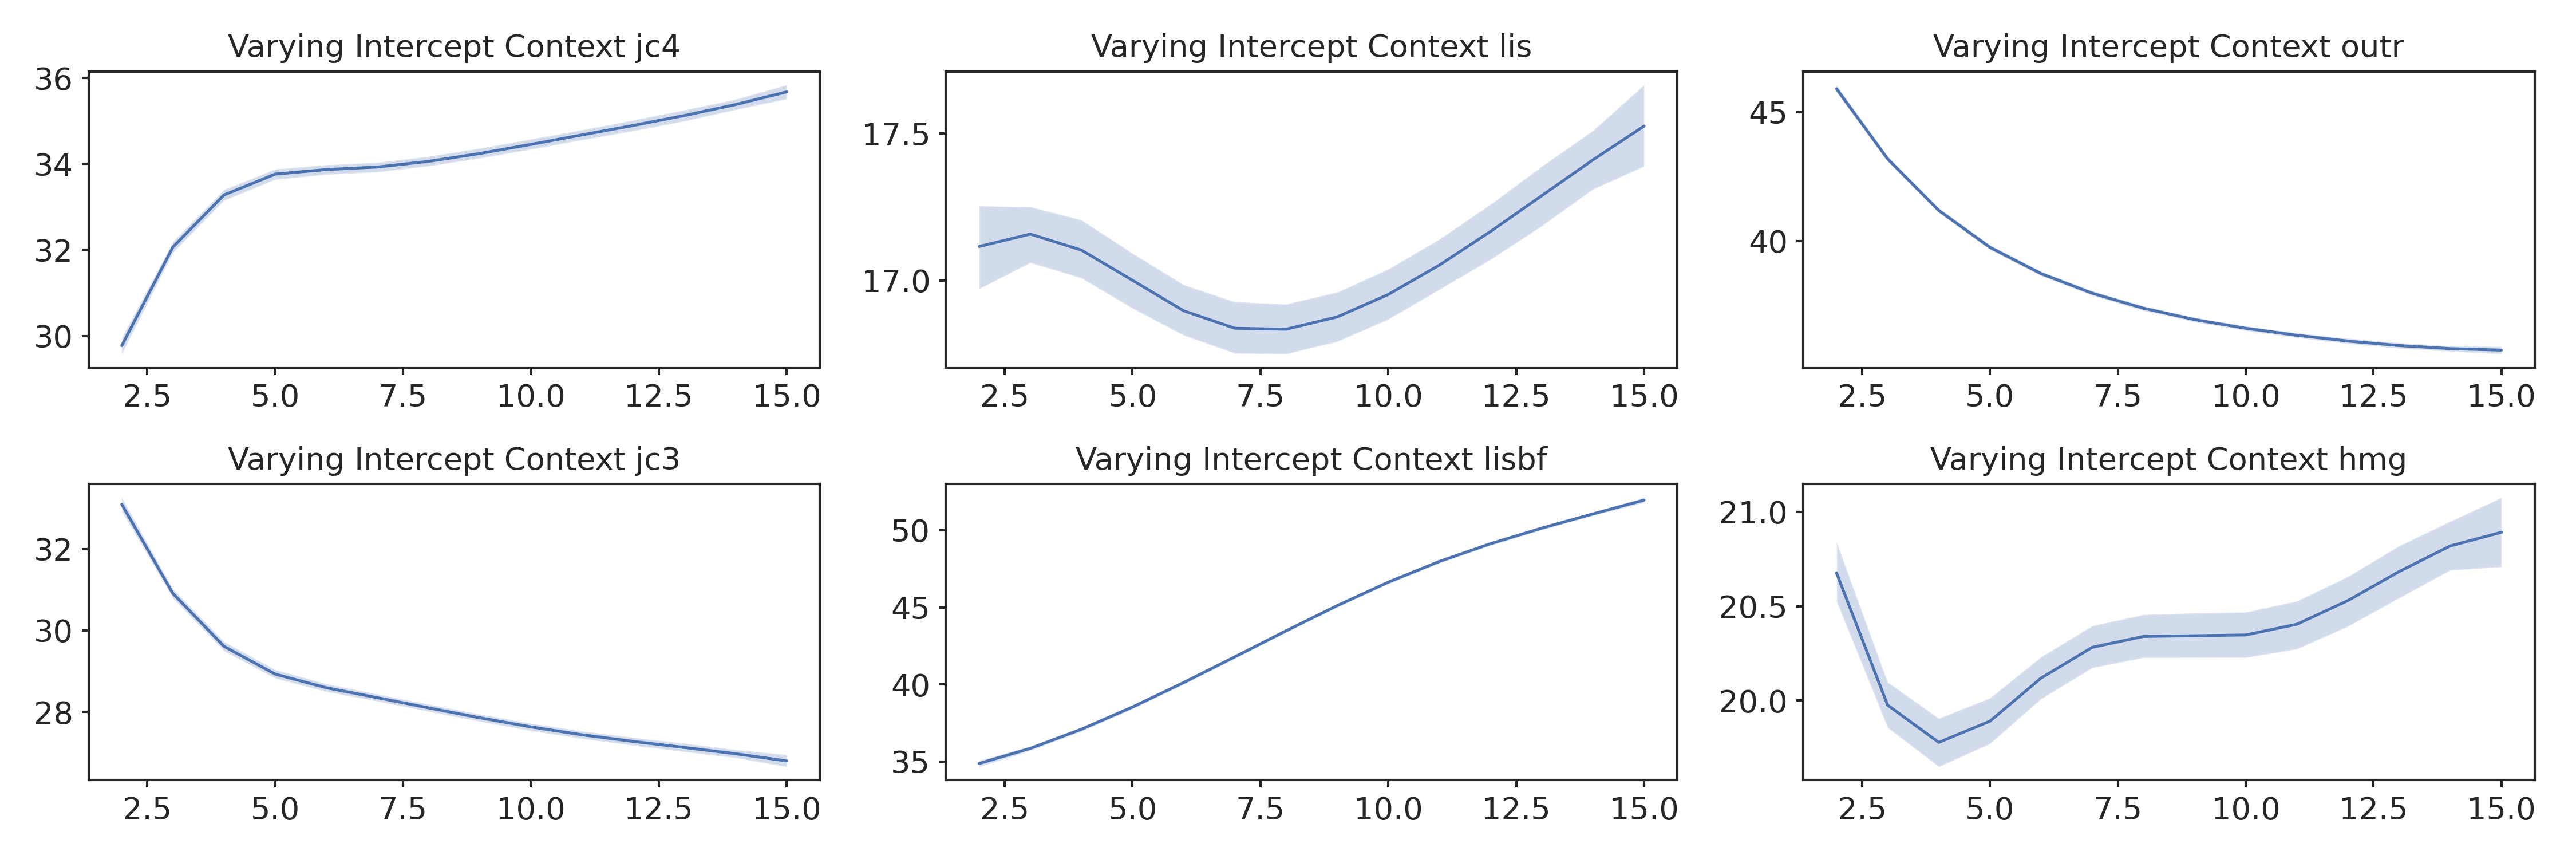
\includegraphics[width=\textwidth]{images/appendix_C/Future Session Activity_interc_3.png}
\caption[\textbf{Future session activity time-varying random intercept}]{Time varying random intercept estimated by the model fitted for the Future Session Activity target.}
\label{interc_acti_3}
\end{figure} \FloatBarrier

\begin{figure}[ht]
\centering
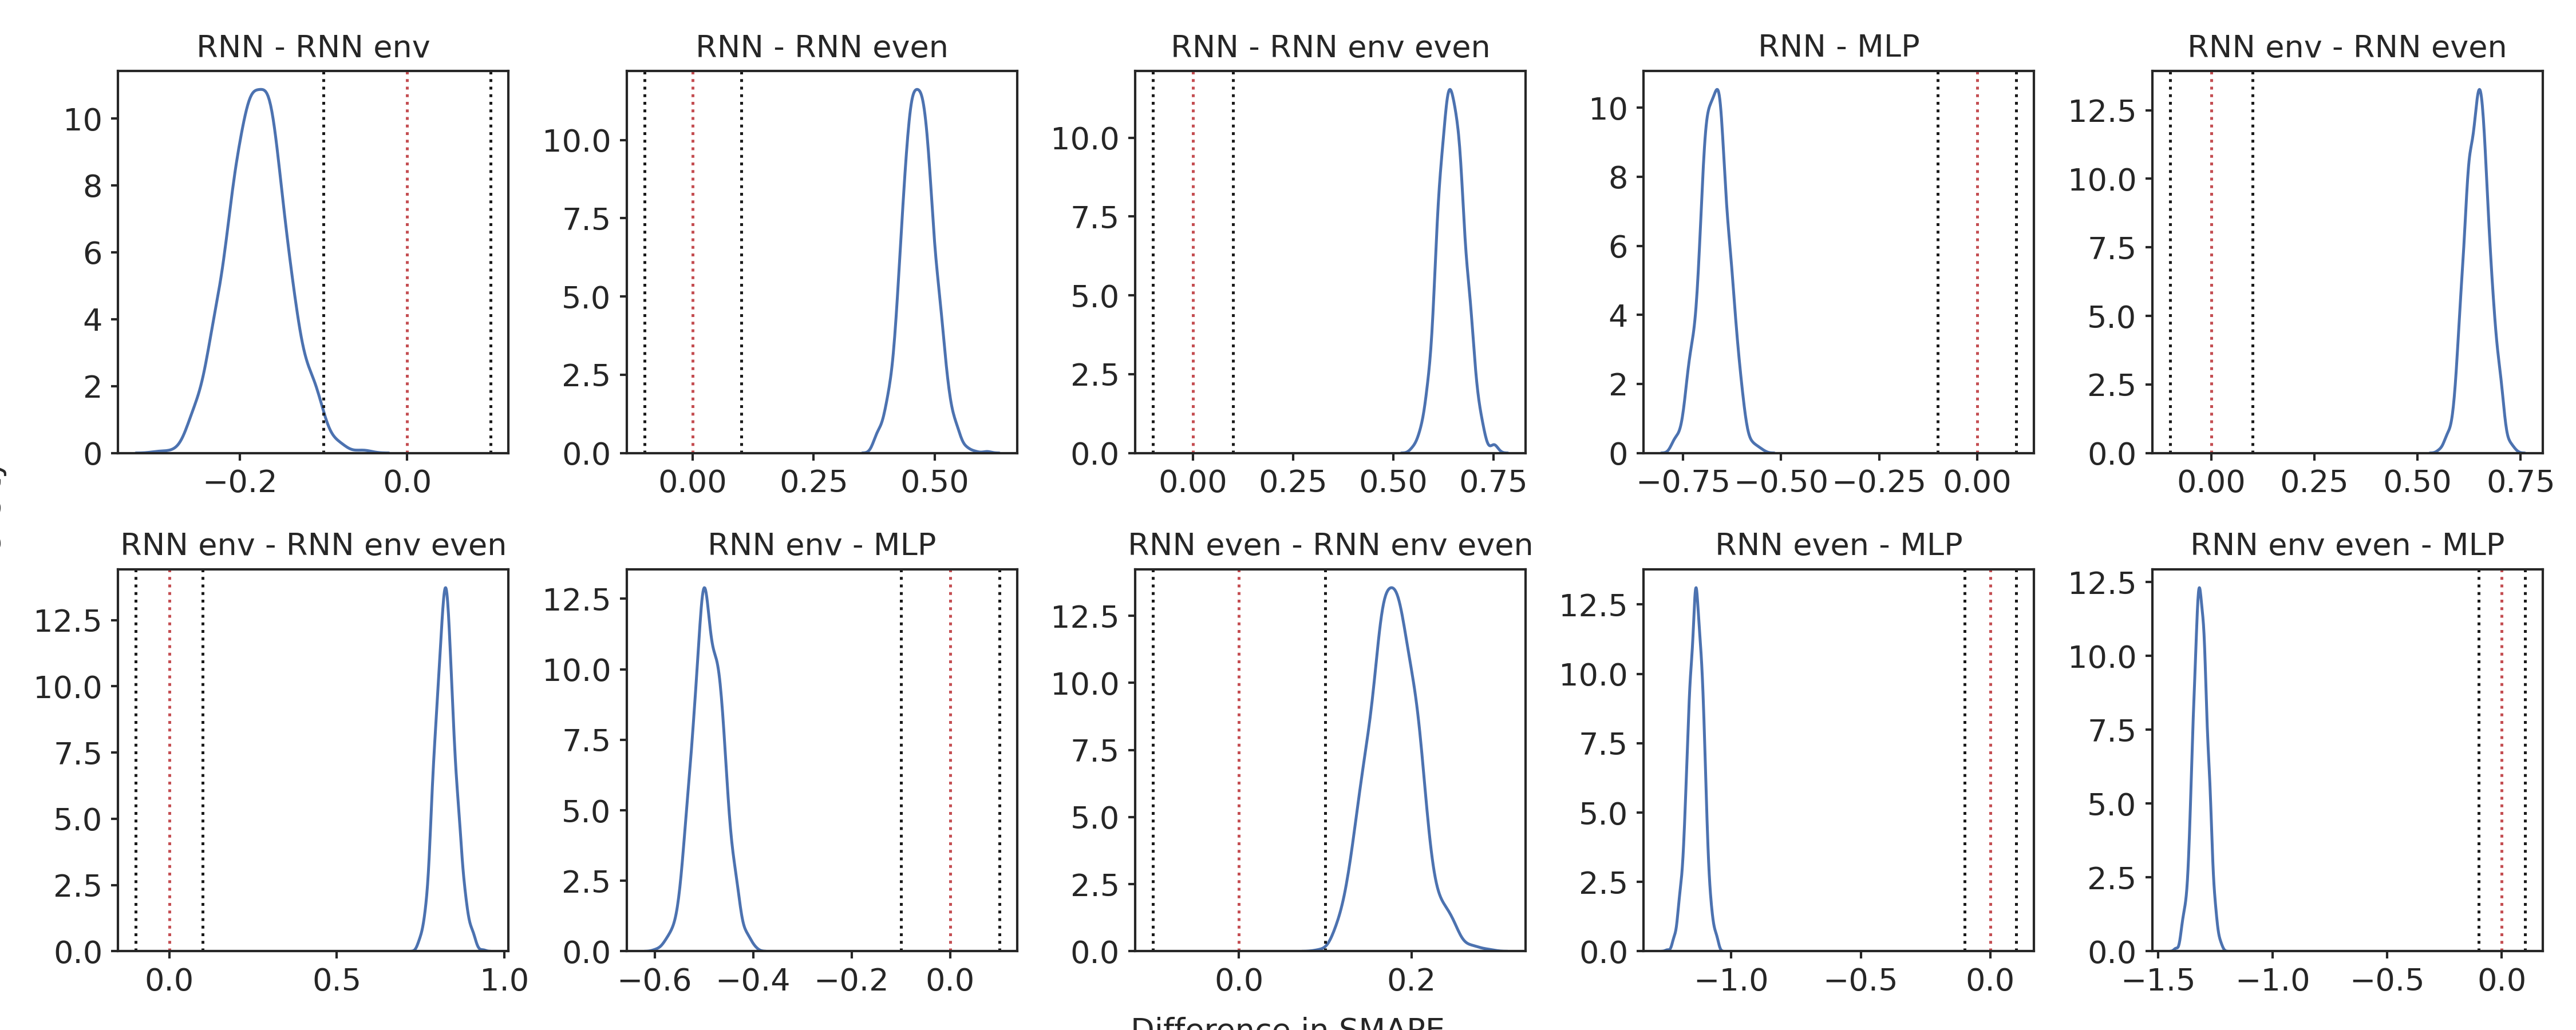
\includegraphics[width=\textwidth]{images/appendix_C/Future_Session_Activity_comp_3.png}
\caption[\textbf{Future session activity pairwise comparisons of model fixed effect}]{Pairwise comparisons of the parameter $\alpha$ (i.e. model slope) estimated by the model fitted for the Future Session Activity target.}
\label{comp_acti_3}
\end{figure} \FloatBarrier

\subsection{Future N° Sessions}
\label{future_no_sess_bayes_3}

\begin{figure}[ht]
\centering
\includegraphics[width=0.5\textwidth]{images/appendix_C/Future N° Sessions_marginals_3.png}
\caption[\textbf{Future N°sessions marginal distributions}]{Marginal distributions for the parameters $\nu$, $\sigma$ estimated by the model fitted for the Future N°sessions target.}
\label{marginals_no_sess_3}
\end{figure} \FloatBarrier

\begin{figure}[ht]
\centering
\includegraphics[width=0.5\textwidth]{images/appendix_C/Future N° Sessions_models_3.png}
\caption[\textbf{Future N°sessions model fixed effect}]{Forest plot of the marginal distributions for the parameter $\alpha$ (i.e. model slope) estimated by the model fitted for the Future N°sessions target.}
\label{model_no_sess_3}
\end{figure} \FloatBarrier

\begin{figure}[ht]
\centering
\includegraphics[width=\textwidth]{images/appendix_C/Future N° Sessions_interc_3.png}
\caption[\textbf{Future N°sessions time-varying random intercept}]{Time varying random intercept estimated by the model fitted for the Future N°sessions target.}
\label{interc_no_sess_3}
\end{figure} \FloatBarrier

\begin{figure}[ht]
\centering
\includegraphics[width=\textwidth]{images/appendix_C/Future_N°_Sessions_comp_3.png}
\caption[\textbf{Future N°sessions pairwise comparisons of model fixed effect}]{Pairwise comparisons of the parameter $\alpha$ (i.e. model slope) estimated by the model fitted for the Future N°sessions target.}
\label{comp_no_sess_3}
\end{figure} \FloatBarrier
